\begin{introduction}

Orientační plány budov jsou pomůckou známou již několik staletí. Pomáhají lidem v~orientaci v~neznámém prostředí a zdůrazňují základní vybavení, např. schodiště, chodby, vstupy či toalety. Nezřídka též obsahují označení místa, kde se člověk na plánu zrovna nachází, což lze považovat za předchůdce modré geolokační ikonky~v~dnešních telefonech.

Další případ je plánek nouzového úniku z~budovy, který zvýrazňuje šipkami trasu k~nejbližšímu východu. Například při útěku před požárem tak lidé z~plánku vyčtou, kterým schodištěm se vydat a kde odbočit. ~Pro nás to~je~opět pěkný předchůdce~indoor~navigace a routování.

S~nástupem smartphonů v~posledních 10 letech začal narůstat význam mapových aplikací. Tyto v~sobě často kombinují digitální mapy se službami geolokace, geocodingu, routování a mnohdy i navigace. Samotná mapa pak může nabízet letecký režim, šikmé snímkování, street view, tématický mód pro cyklisty apod. Samozřejmostí jsou pak business listingy s~možností recenzování.

Mezi další vlastnosti moderních aplikací patří hlášení polohy~uživatelů, které je cennou informací pro podnikání, zejména polohově cílenou reklamu. Zjišťování~návyků lidí poskytuje mnoho nových možností v~oblasti~služeb. Získáváním výstupů z~polohových dat se zabývá nově vzniklý vědní obor Location Intelligence, který samozřejmě využívá principy známé znalostnímu inženýrství\footnote{anglicky Business Intelligence}.

Indoor mapy jsou doménou několika posledních let. V~roce 2012 s~nimi přišla na scénu společnost Google\cite{zdroj1}.~O~dva roky později naznačil vývoj Apple, načež mnohé zpravodajské portály předvídaly\cite{zdroj2}, že indoor mapping bude \uv{příští velká věc}\footnote{V originále: the next big thing}.

Indoor mapy a geolokace představují~velkou technologickou výzvu pro současný věk.

V~naší~práci se detailně zabýváme problematikou indoor map, možnostmi platformy OpenStreetMap\footnote{Stránka projektu na \href{http://openstreetmap.org}{openstreetmap.org}, stránka české komunity na \href{http://openstreetmap.cz}{openstreetmap.cz}}~a úpravou webového editoru~iD.

V~první kapitole uvádíme definici problému a shrnujeme přístup současných služeb. Ve druhé se zaměřujeme na službu OpenStreetMap (OSM) -- její architekturu, dostupné editory, dosavadní přístup k~indoor a návrh vhodné metodiky pro tvorbu. Ve třetí kapitole pak popisujeme architekturu editoru iD, proces návrhu uživatelského rozhraní pro indoor a samotné implementace. V~poslední kapitole pak shrnujeme výsledky a uvádíme možná využití ve veřejných budovách včetně konkrétního příkladu ČVUT.

V~naší práci užíváme terminologii zaběhnutou v~české komunitě projektu OpenStreetMap.~Čtenář by jí měl věnovat pozornost, protože v~dalším textu jí četně využíváme.

Terminologie užitá v~této práci:

\begin{itemize}

\item
  souřadnice - zeměpisné souřadnice, typicky ve formátu WGS84~(pokud není blíže určeno)
\item
  geolokace - zaměření polohy uživatele, typicky pomocí GPS
\item
  indoor geolokace - zaměření polohy uživatele pomocí jiných prostředků (viz kapitola 1.2.)
\item
  indoor mapy - mapy vnitřků budov
\item
  routování - nalezení trasy mezi dvěma fyzickými body
\item
  geocoding - nalezení souřadnic dle zadané adresy (a reverzní geocoding obráceně)
\item
  navigace - proces určení polohy a sestavení pokynů pro následování nalezené trasy
\item
  business listing~- záznam obchodu v~mapové aplikaci, typicky v~podobě umístěné ikonky na konkrétních souřadnicích v~mapě
\item
  POI (point of interest) - bod zájmu v~mapě, např. nemocnice, zastávka MHD či business listing
\item
  street view~-- panoramatické fotografie v~uliční úrovni
\end{itemize}

\end{introduction}



\chapter{Problematika indoor map}\label{problematika-indoor-map}

Hlavním specifikem indoor map je nutnost oddělení~jednotlivých pater, tedy zobrazení jedné polohy v~různých výškách.~Tím se výrazně odlišují od venkovních map i orientačních plánků, které zobrazují vždy jen jeden pohled shora.

Termín indoor mapy používáme~z~toho důvodu, že~se nejedná pouze o~plány budov, ale všech vnitřních prostor. ~To zahrnuje i podzemní prostory, zejména stanice metra, či vlaková nadraží s~podchody apod.

V~kartografii se plán od mapy liší tím, že zanedbává zakřivení Země. My ho ovšem používáme v~laickém významu, tedy pro všechny detailní mapy malého území. U~webových plánů budov se ve většině případů bude technicky jednat o~mapy, neboť využívají zeměpisných souřadnic a stejné mapové projekce jako (okolní) mapa venkovní.

V~této kapitole uvedeme současné služby a nastíníme i teoretické možnosti související s~indoor geolokací.


                      \begin{figure}
                    	  \centering
                    \subfloat[\label{obr1a}]
                    {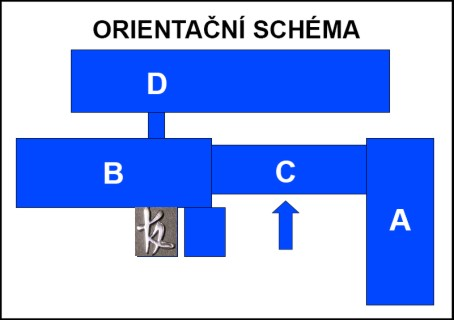
\includegraphics[width=.5\linewidth]{img/1a-orientacni-fsv.jpg}}\hfill
                    \subfloat[\label{obr1b}]
                    {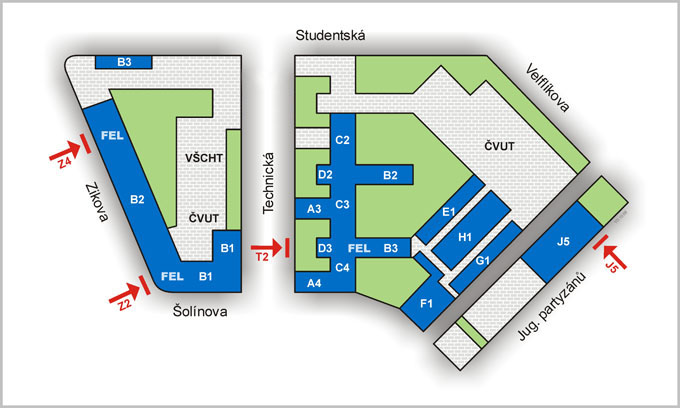
\includegraphics[width=.5\linewidth]{img/1b-orientacni-fel.jpg}}\hfill
                    \subfloat[\label{obr1c}]
                    {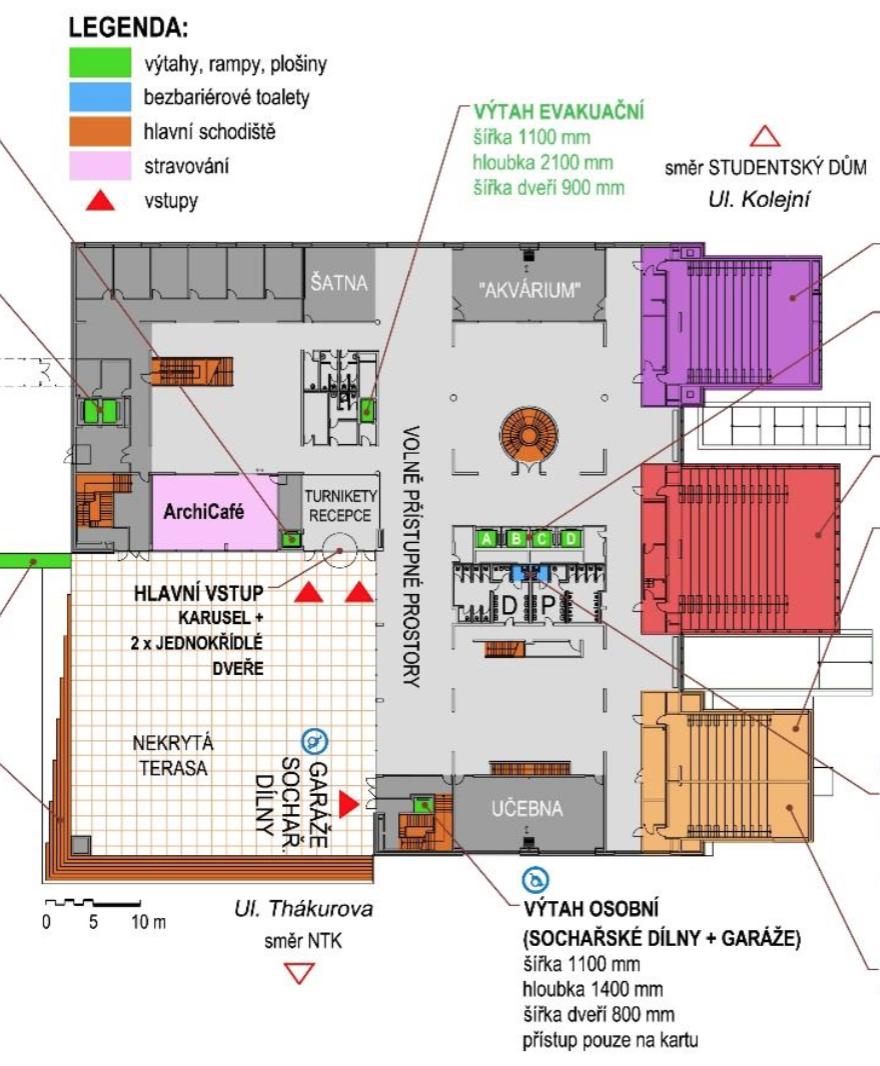
\includegraphics[width=.75\linewidth]{img/1c-orientacni-fa.png}}

                    \caption{Orientační plány budov ČVUT -- FSv\cite{zdroj3}~(a); FEL\cite{zdroj4}~(b); a FA\cite{zdroj5}~(c)}
                    \label{obr1}
                    \end{figure}
                    



\section{Současné indoor služby}\label{souux10dasnuxe9-indoor-sluux17eby}

Současným indoor službám přirozeně dominují velcí hráči na poli webových map. V~posledních letech, též díky nástupu autonomních vozidel, proběhlo několik zajímavých akvizic. Pojďme si tedy shrnout \uv{kdo je kdo}:

\begin{itemize}

\item
  TomTom -- v~roce 2008 akvizice firmy Teleatlas, nyní poskytuje data pro Apple Maps a Uber. Od roku 2014 navázal ohledně indoor map partnerství s~firmou Micello.\cite{zdroj6}\cite{zdroj6b}
\item
  Micello -- vznikla v~roce 2007 v~Sillicon Valley a nyní má zmapováno největší množství indoor prostor. Data nabízí zejména do aplikací třetích stran.\cite{zdroj7}
\item
  Google -- do roku 2008 používal data TeleAtlasu, později využívá vlastní koupené či půjčené datasety\cite{zdroj8}. Indoor mapy nyní implementuje do svých Google Maps na všech platformách.
\item
  Here -- v~roce 2011 vzniklo jako Nokia Ovi Maps akvizicí firmy NAVTEQ. V~prosinci 2015 koupeno německými automobilkami od firmy Nokia už pod názvem Nokia Here Maps\cite{zdroj9}\cite{zdroj9b}. Firma NAVTEQ uveřejnila své indoor řešení na konferenci Nokia World 2010\cite{zdroj10}, ovšem Here Maps již tato data na webu nezobrazují.
\item
  Microsoft -- služba Bing Maps oznámila indoor mapy v~roce 2011 pod názvem Venue Maps\cite{zdroj11}. Mapová data nadále vlastní, ale divize tvorby byla odprodána firmě Uber (poté,~co tato prohrála boj o~Here Maps).\cite{zdroj12}
\end{itemize}

Zcela vyčerpávající přehled lze najít v~tabulce \uv{The Indoor Navigation Market}\cite{zdroj13}~od společnosti BuildingLayer.

\subsection{Google Maps Indoor}\label{google-maps-indoor}

Google se stal konkurencí v~oblasti webových map~akvizicí několika startupů v~roce 2004~--~zejména firmy Keyhole, která dala za vznik legendární aplikaci Google Earth. Díky uvolnění API, mobilním aplikacím (včetně spolupráce s~prvními telefony iPhone v~letech 2007-2012) a Street View se začal Google stávat jedním z~hlavních hráčů na trhu. Celý poutavý příběh můžete najít ve zdroji.\cite{zdroj14}

Indoor mapám se začal věnovat v~roce 2011, kdy spustil prohlížeč v~rámci své aplikace pro Android.\cite{zdroj15}~Na své projektové stránce\footnote{\href{https://www.google.com/maps/about/partners/indoormaps/}{www.google.com/maps/about/partners/indoormaps/}} Google vybízí instituce, aby samy nahrály obrázky podlažních plánů a zarovnaly je vůči satelitní mapě. Samotnou vektorizaci pak dělá Google sám.\cite{zdroj16}~V~ČR tato služba zatím není v~provozu, ale jednotlivé instituce i tak mohou své plány poslat.\cite{zdroj17}


                      \begin{figure}
                     \centering
                    \subfloat[\label{obr2a}]
                    {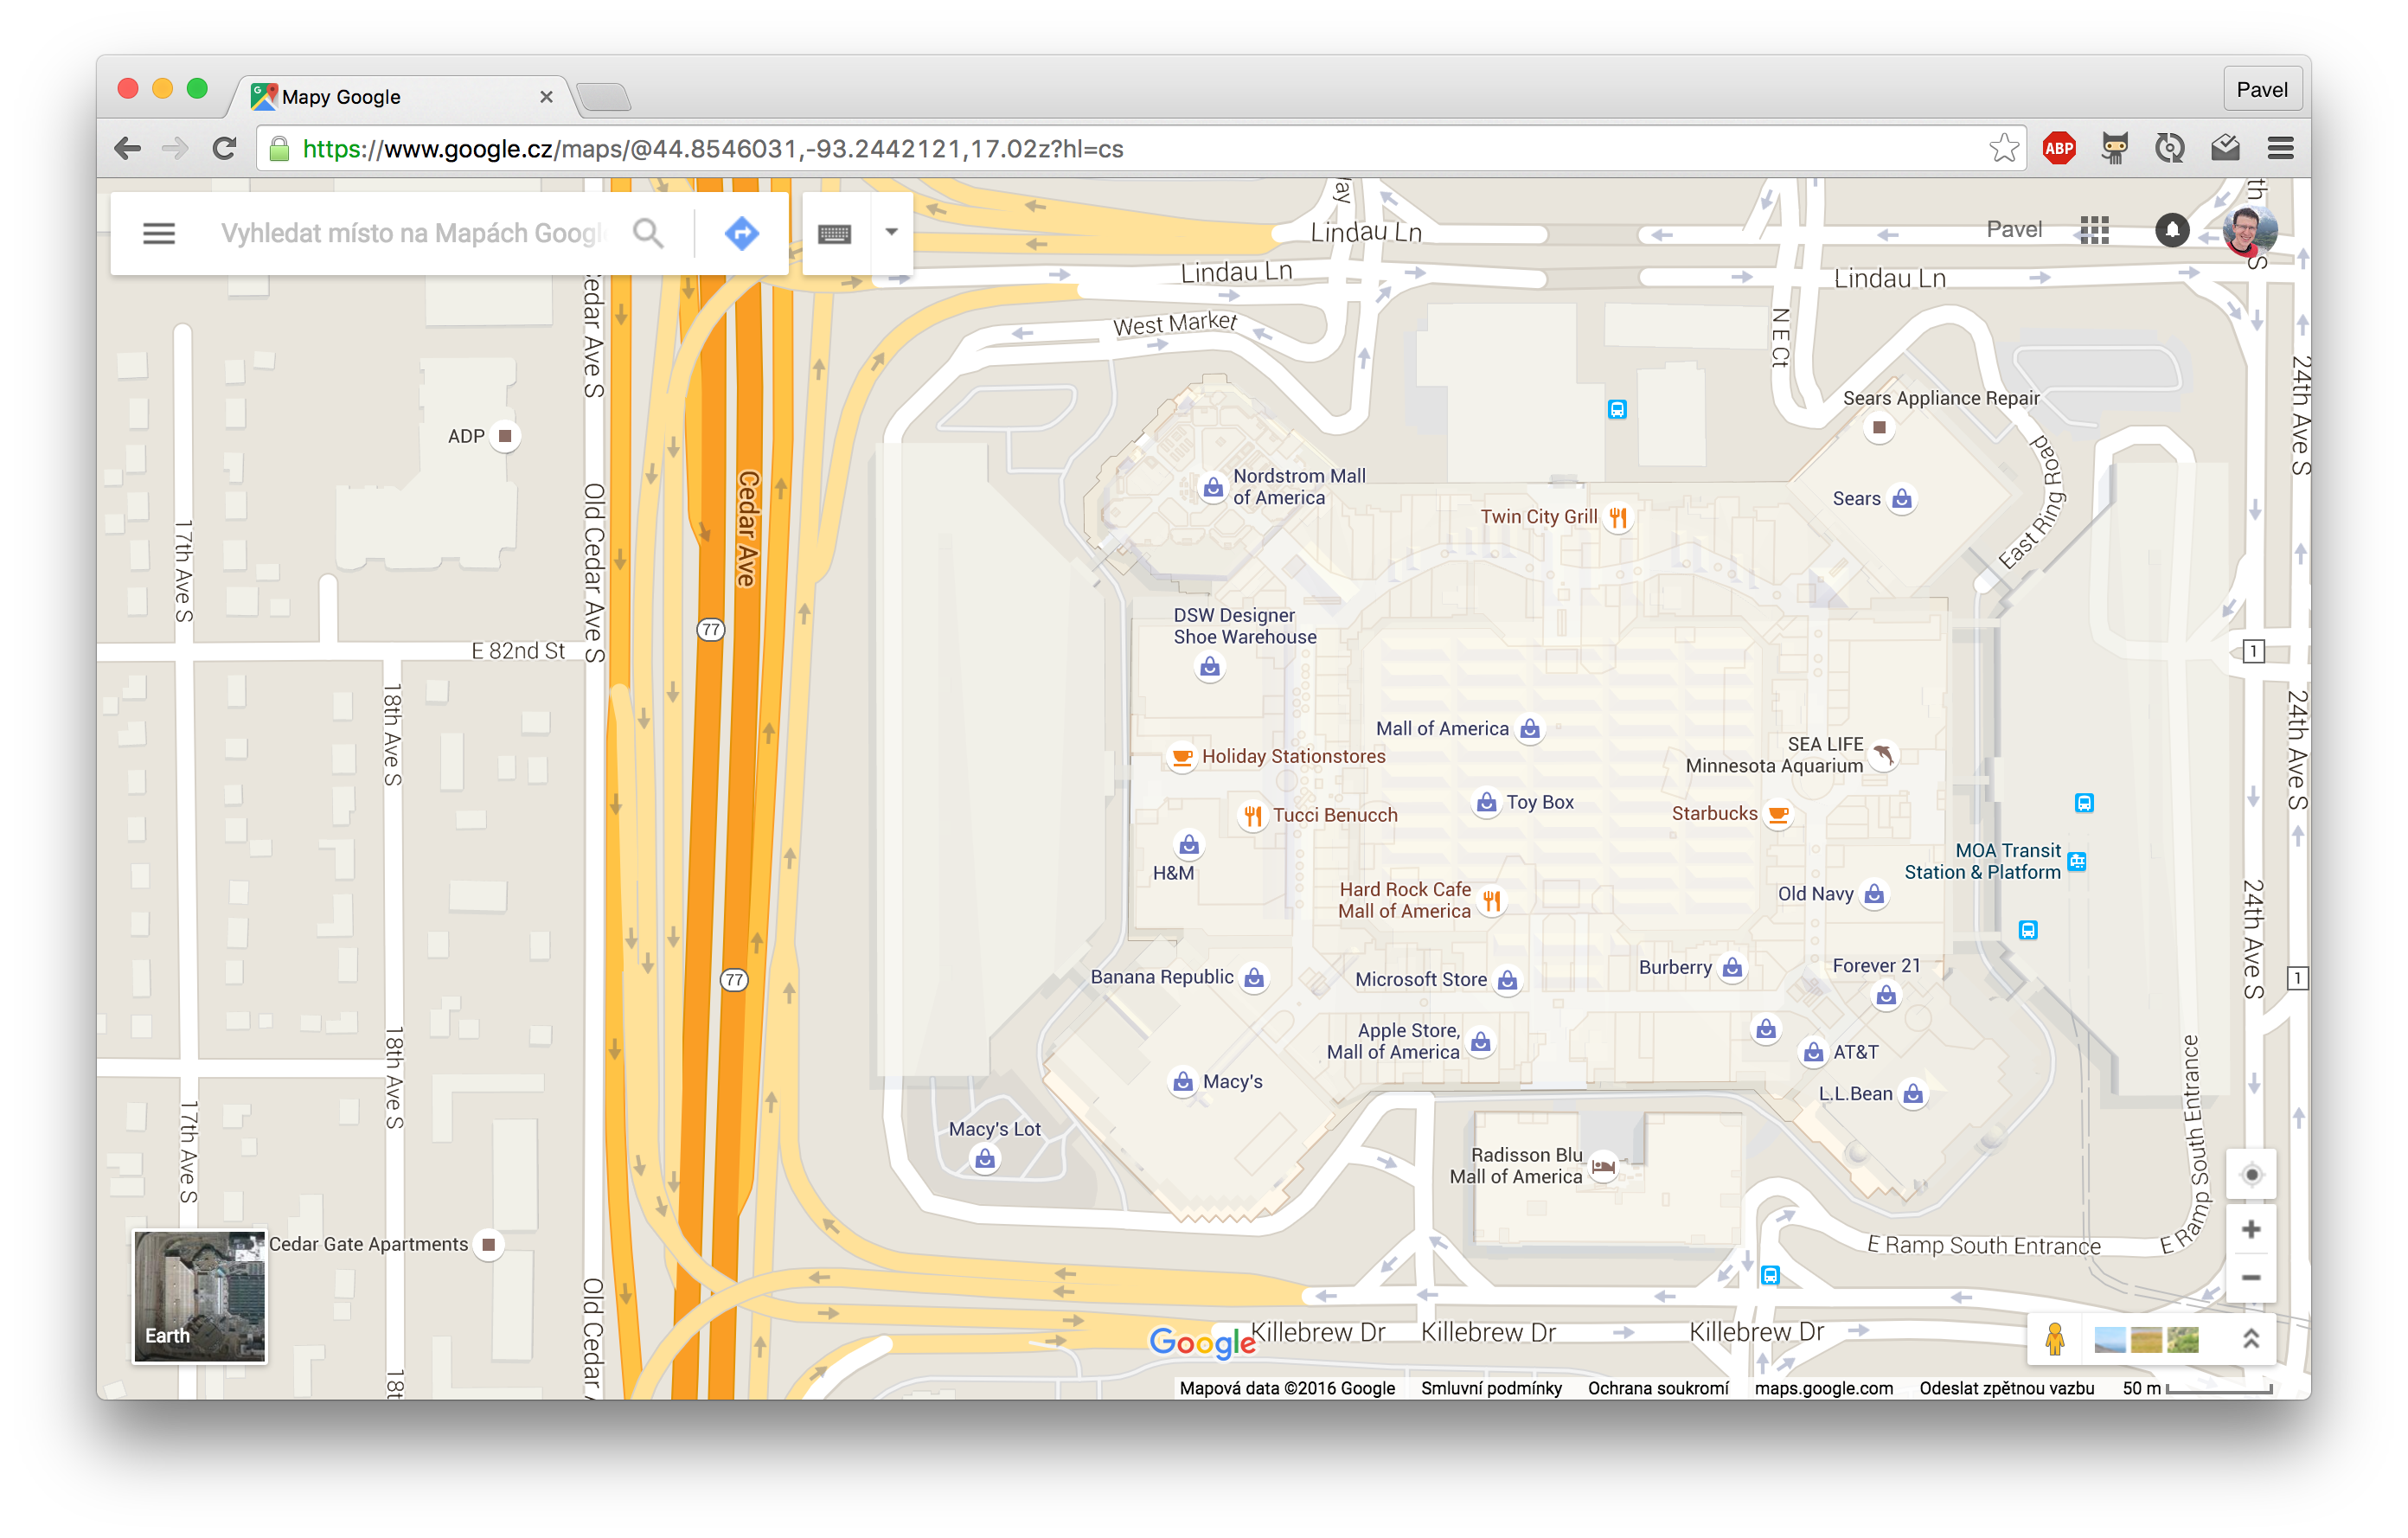
\includegraphics[width=.5\linewidth]{img/2a-gmaps-moa.png}}\hfill
                    \subfloat[\label{obr2b}]
                    {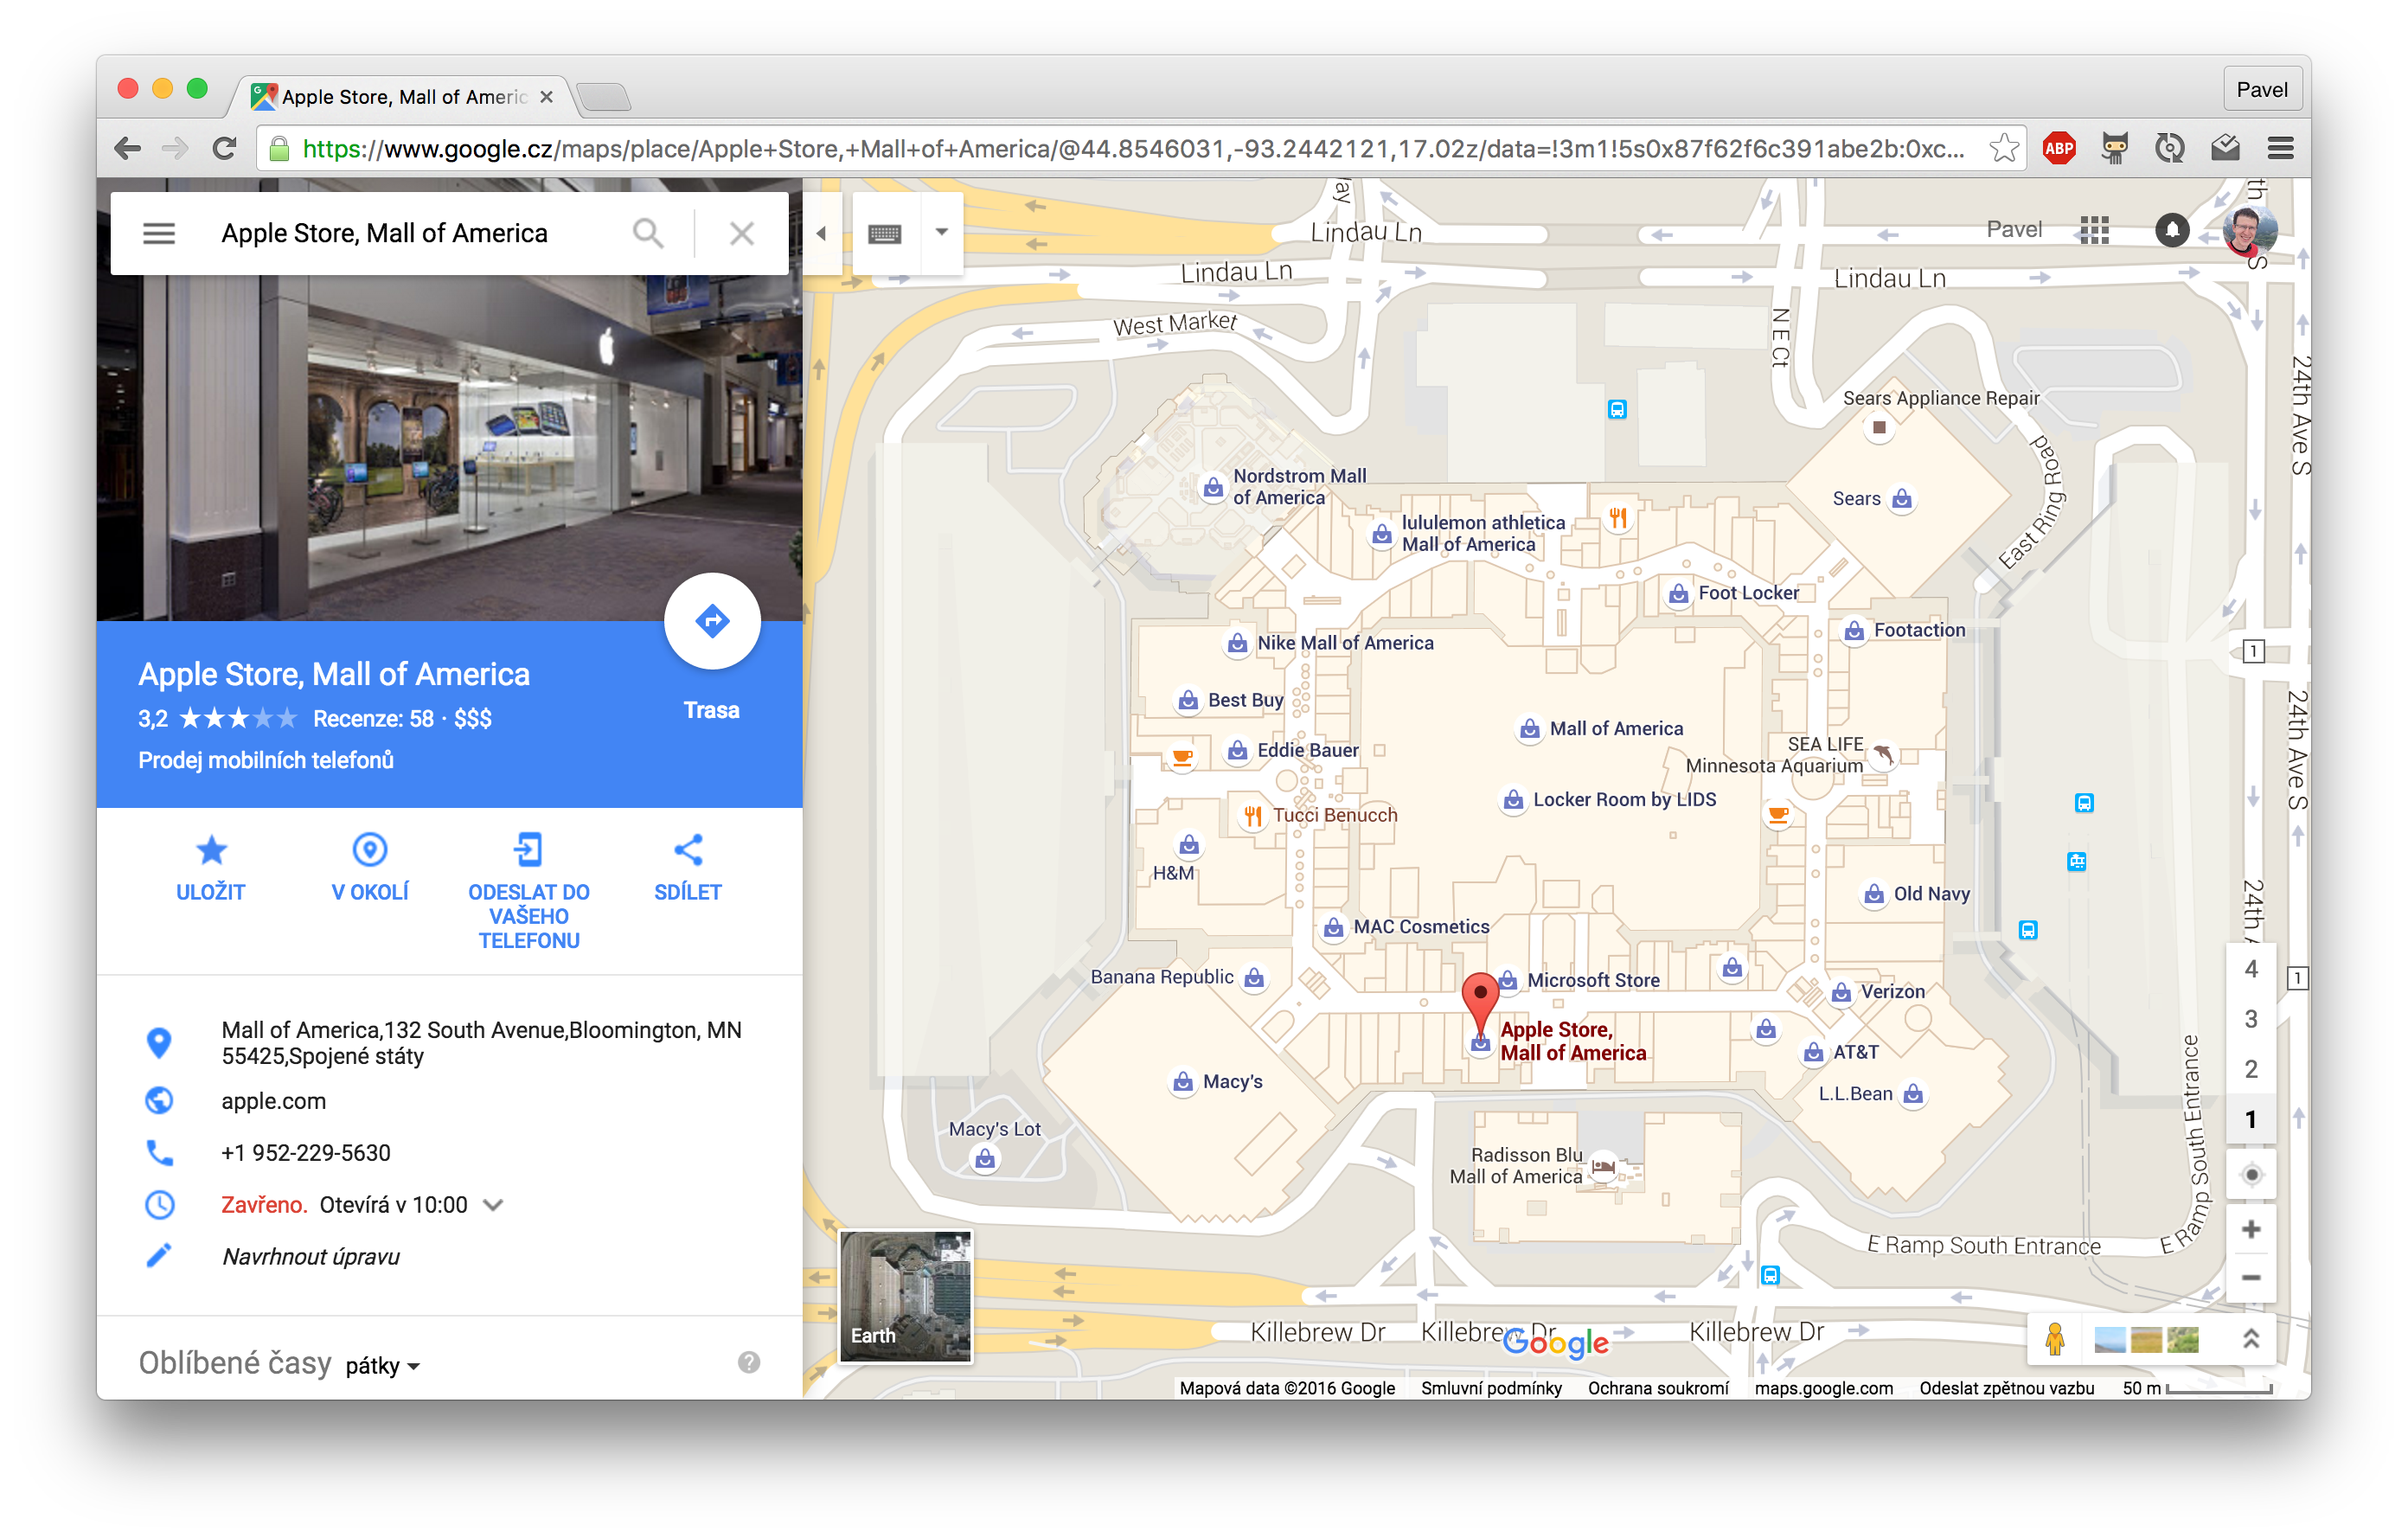
\includegraphics[width=.5\linewidth]{img/2b-gmaps-moa-1-indoor.png}}\hfill
                    \subfloat[\label{obr2c}]
                    {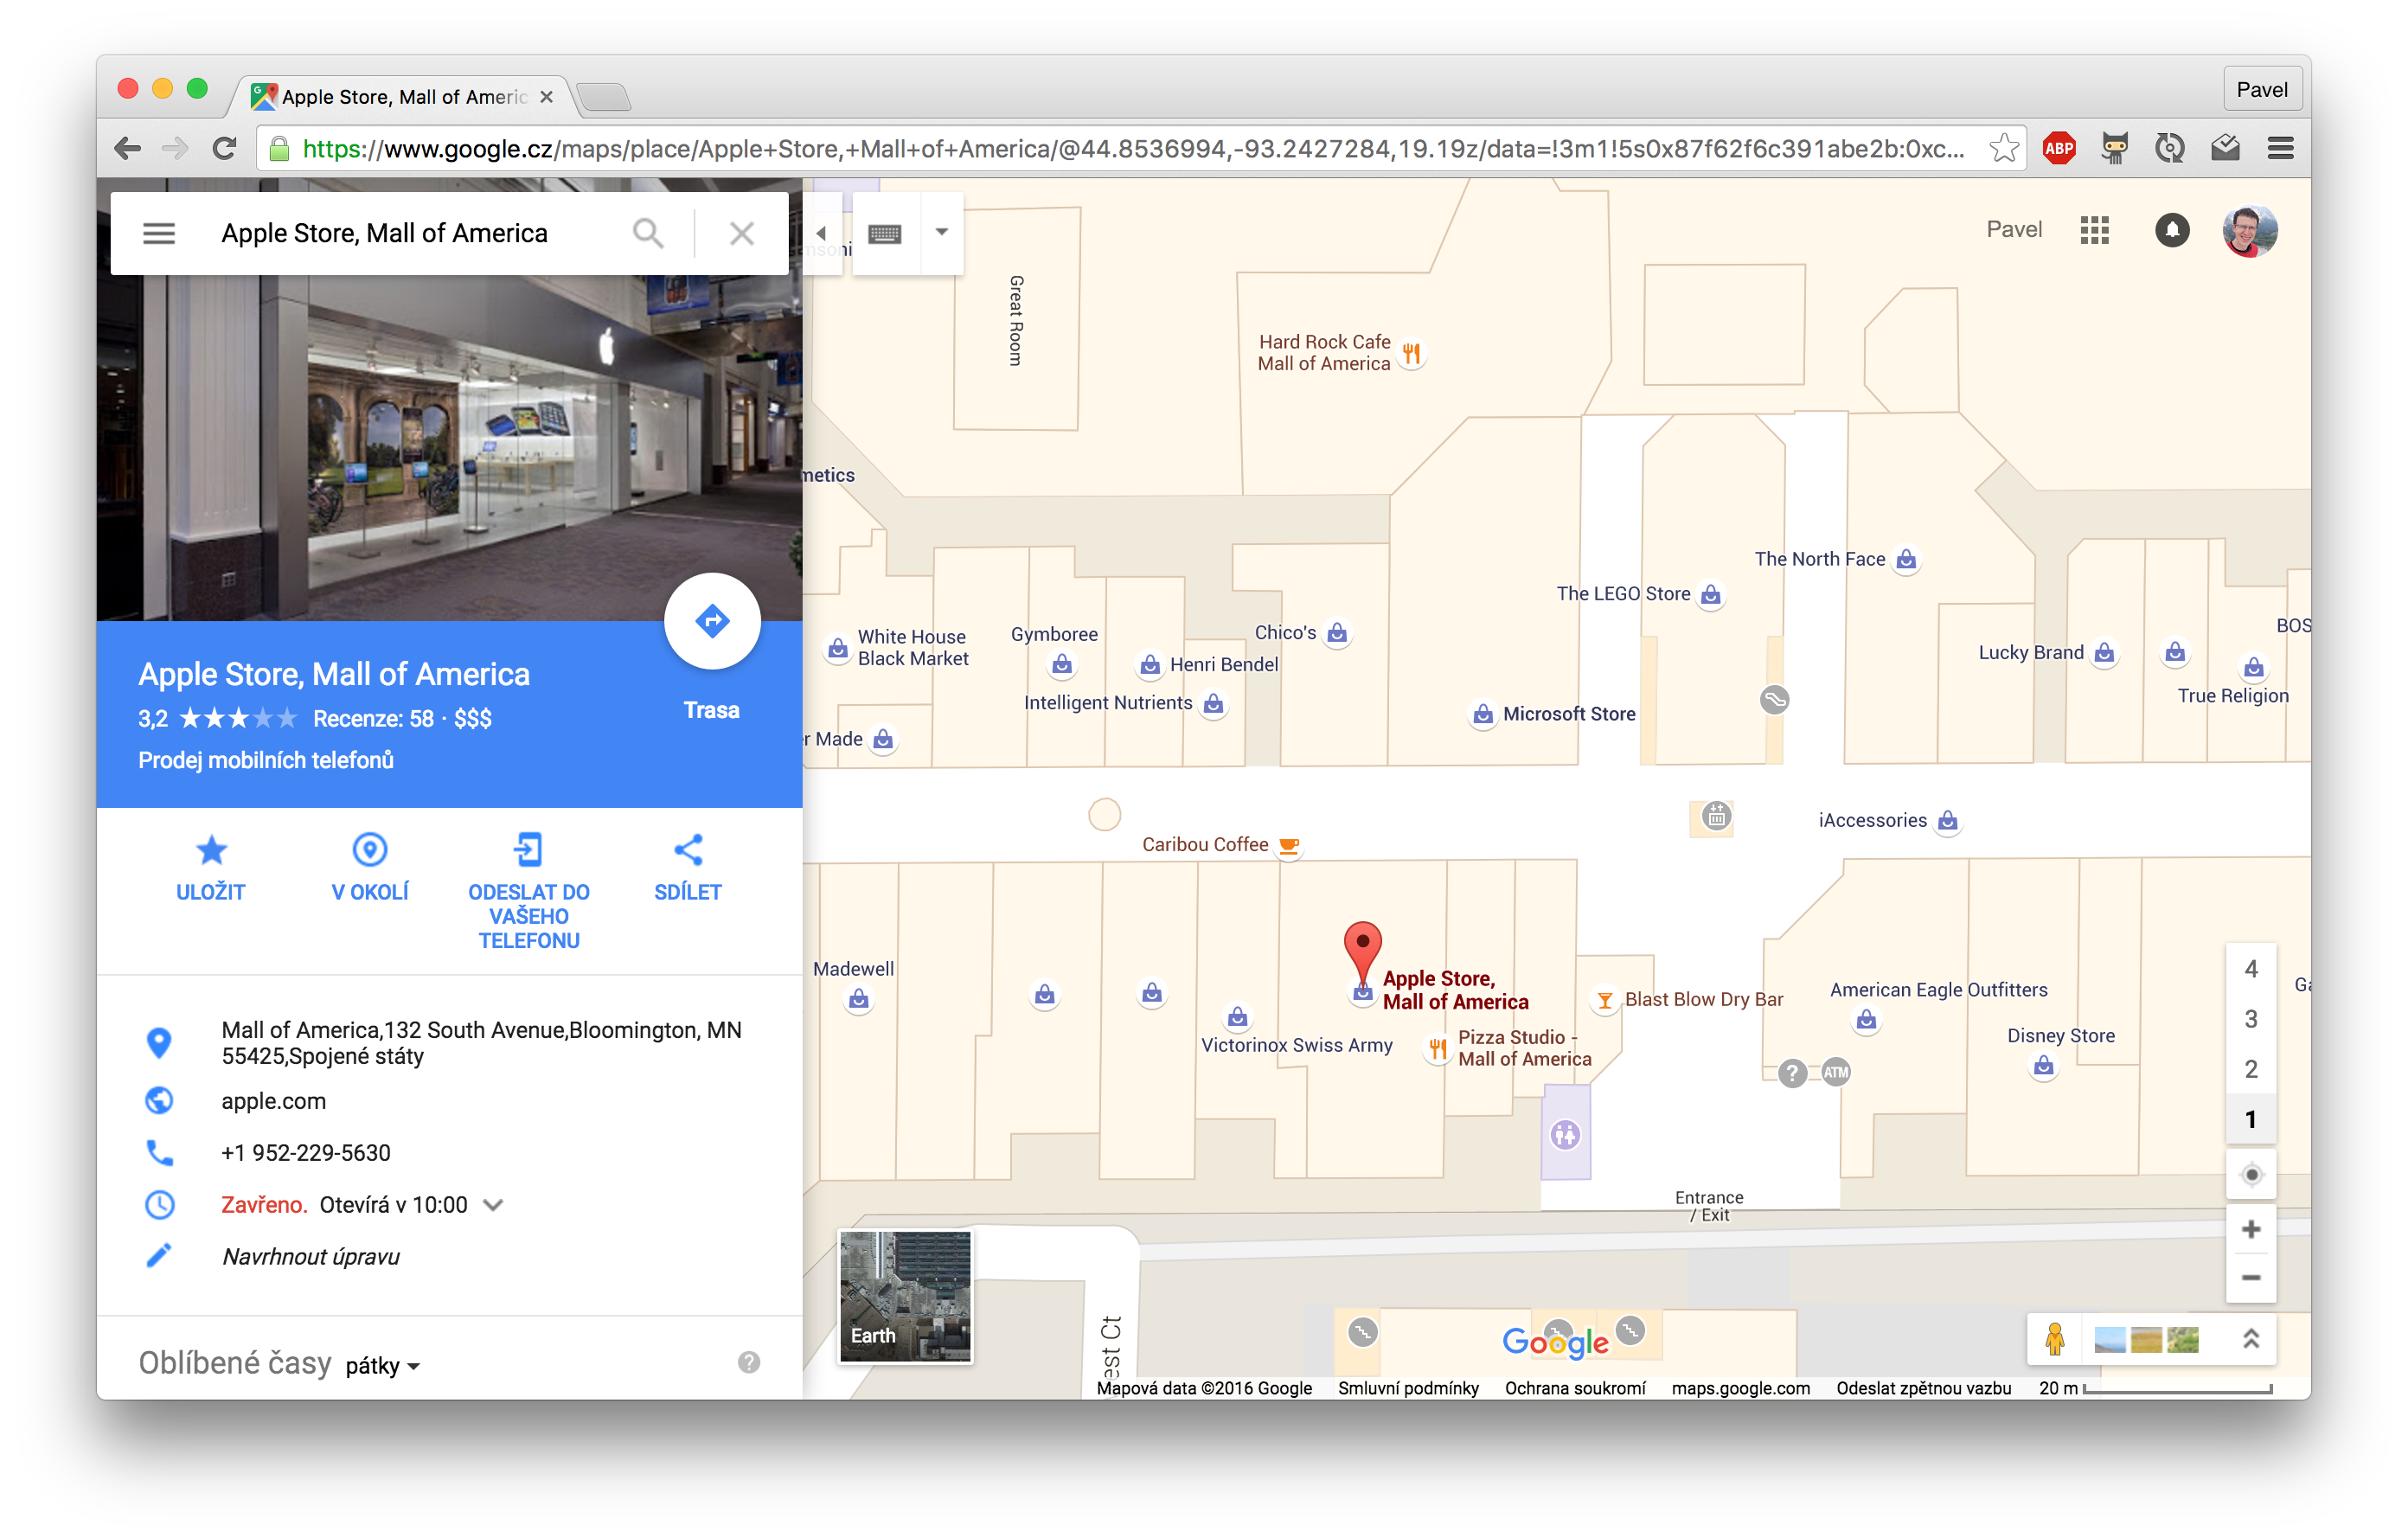
\includegraphics[width=.5\linewidth]{img/2c-gmaps-moa-2.png}}

                    \caption{Zobrazení klasické mapy~v~Google Maps (a); přepnutí do indoor zobrazení (b); přiblížení (c)}
                    \label{obr2}
                    \end{figure}
                    

Indoor zobrazení se aktivuje jednak při dostatečném přiblížení mapy, jednak~při kliku na business listing, který je umístěn ve~zmapované budově. V~indoor zobrazení se též ukáže přepínač pater budovy.

\subsection{Apple Maps Indoor}\label{apple-maps-indoor}


                      \begin{figure}
                    	  \centering
                    \subfloat[\label{obr3a}]
                    {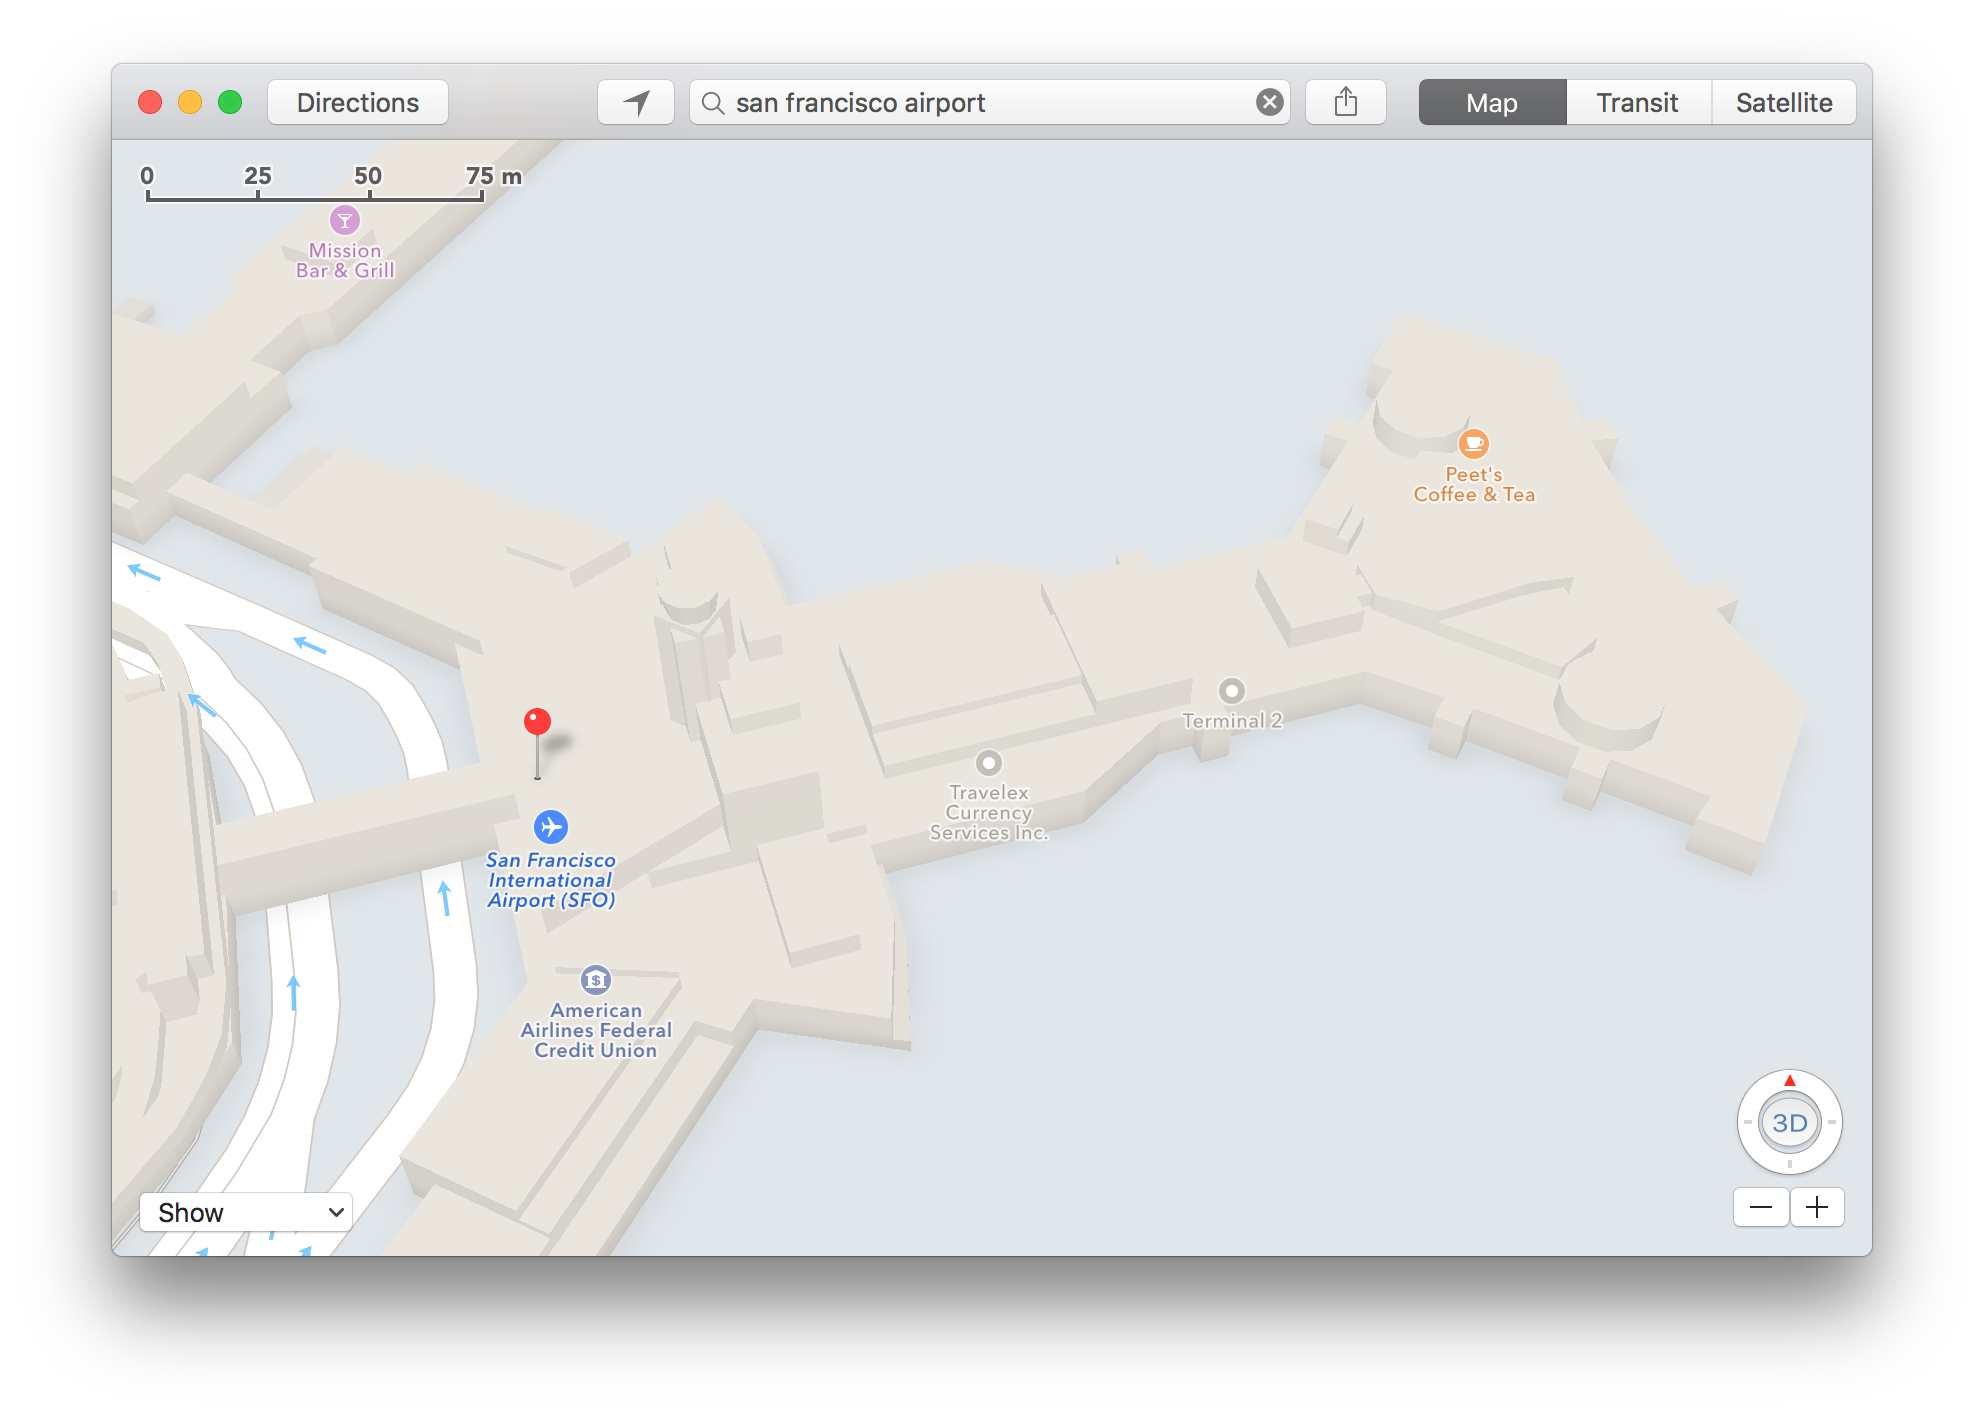
\includegraphics[width=.5\linewidth]{img/3a-apple-san-fran.png}}\hfill
                    \subfloat[\label{obr3b}]
                    {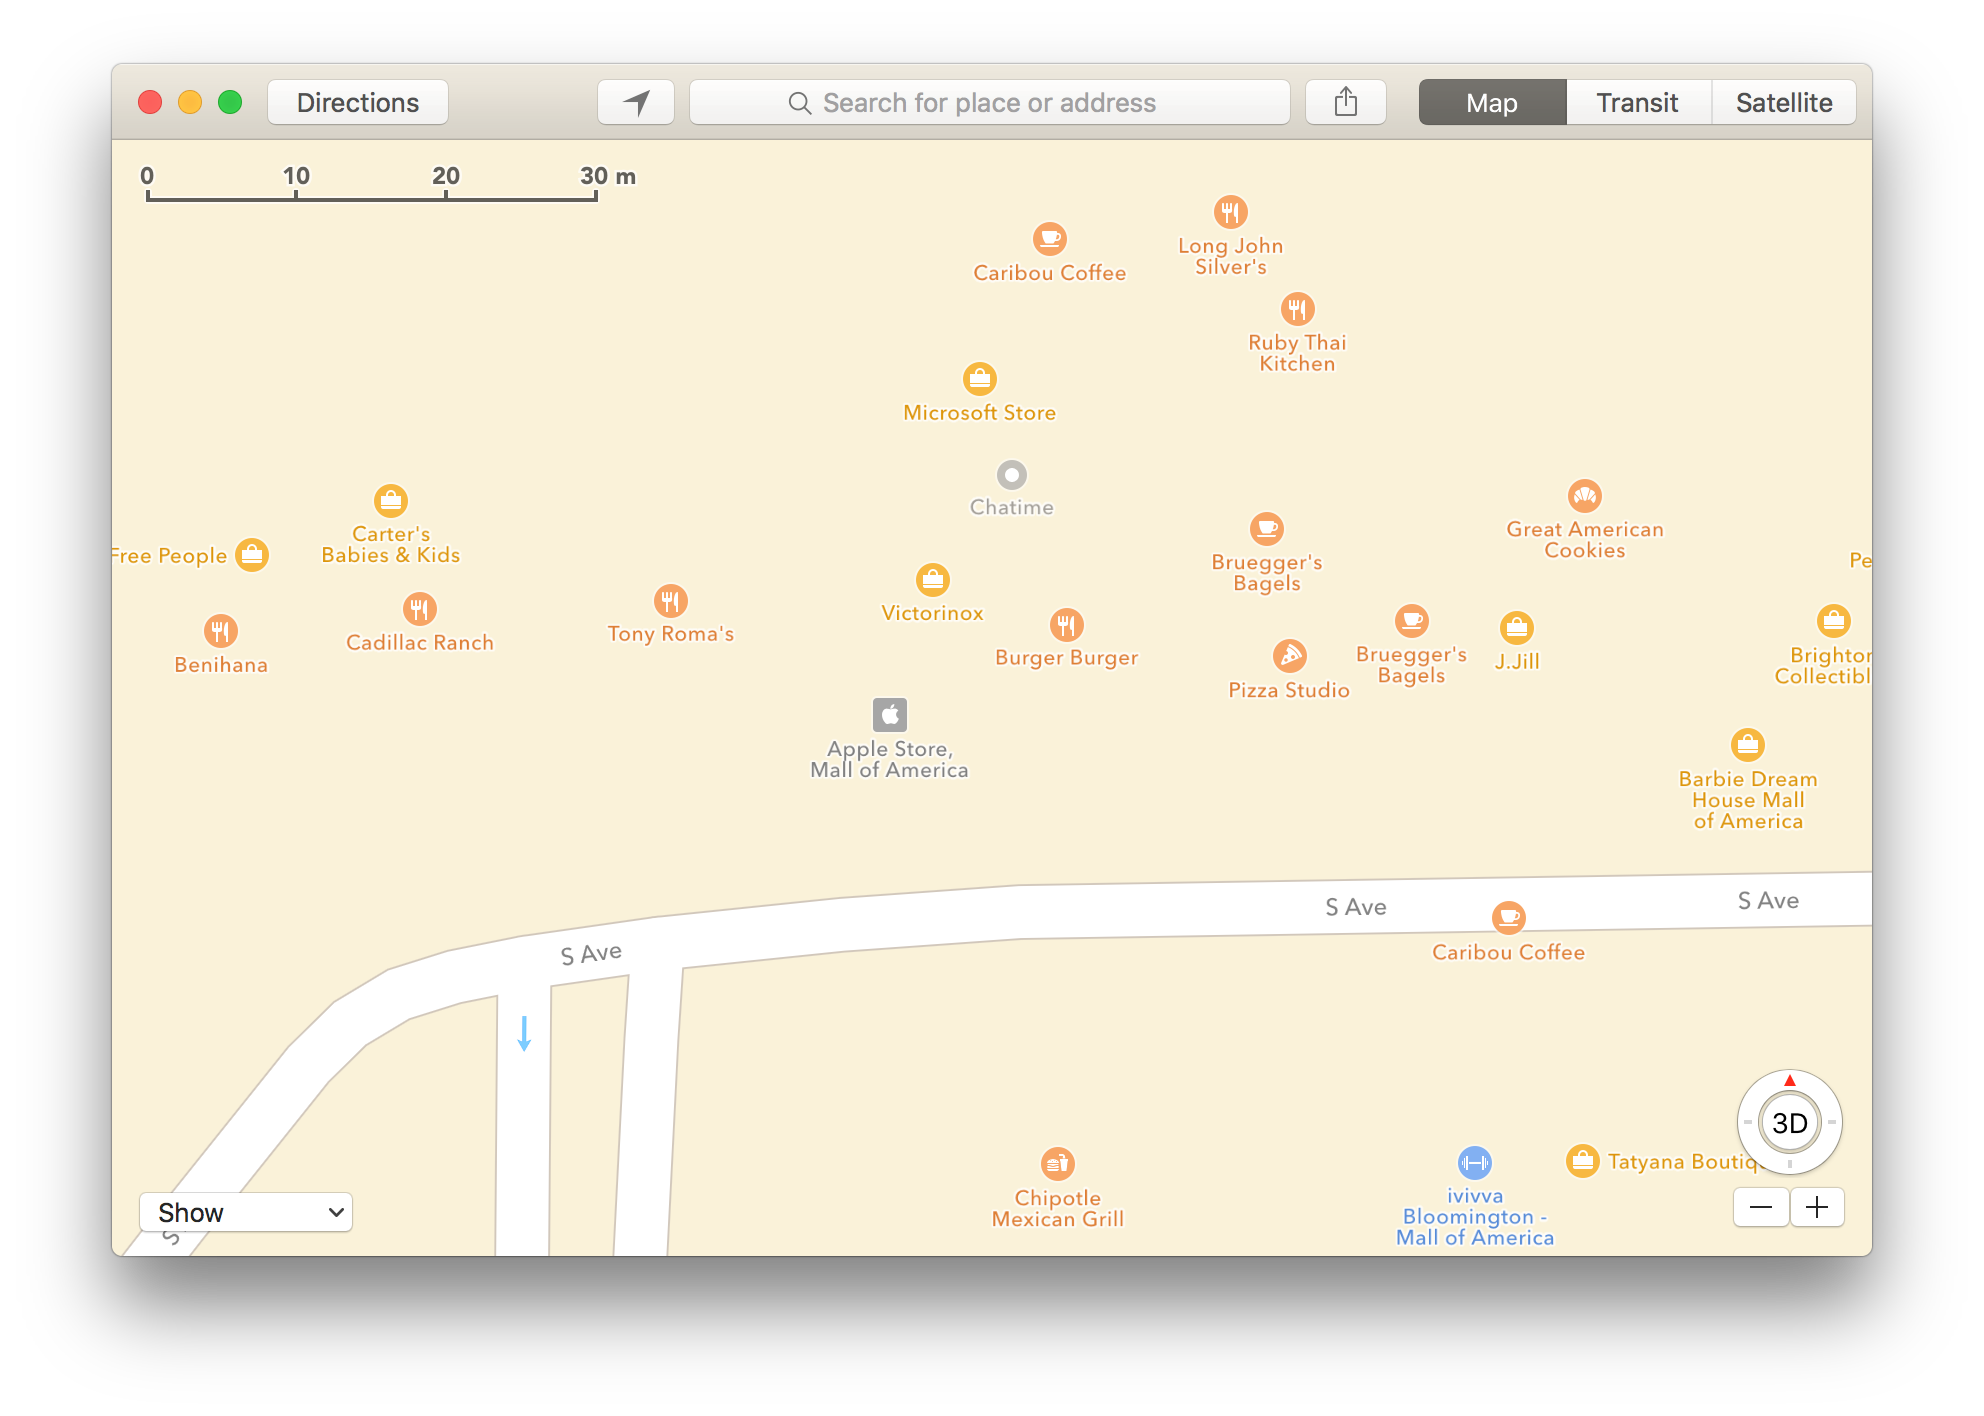
\includegraphics[width=.5\linewidth]{img/3b-apple-moa.png}}

                    \caption{3D obrys budovy~v~Apple Maps~bez indoor plánu (a); pouze zarovnané ikony (b)}
                    \label{obr3}
                    \end{figure}
                    

Společnost Apple v~současné době indoor mapy neposkytuje. Ovšem dle náznaků firma službu připravuje. V~listopadu 2015 Apple zveřejnil aplikaci \uv{Indoor Survey}\cite{zdroj18}, která umožňuje správcům velkých nákupních center provést zaměření pro vnitřní geolokaci. Pomocí aplikace se v~budově zaměří referenční body a k~nim uloží otisk WiFi i Bluetooth vysílačů a dat ze senzorů iPhonu. Vice o~speciálních geolokačních Bluetooth vysílačích Apple iBeacon najdete v~kapitole 1.2.

V~průběhu roku 2015 též zarovnala umístění business listingů na jejich správné souřadnice v~rámci budov nákupních center\cite{zdroj19}.~

Není jisté, zda Apple bude tvořit vlastní indoor mapy, nebo jen využívat přesnou indoor geolokaci pro aplikace třetích stran\cite{zdroj20}.

\subsection{Microsoft Bing Maps}\label{microsoft-bing-maps}


                      \begin{figure}
                    	  \centering
                    \subfloat[\label{obr4a}]
                    {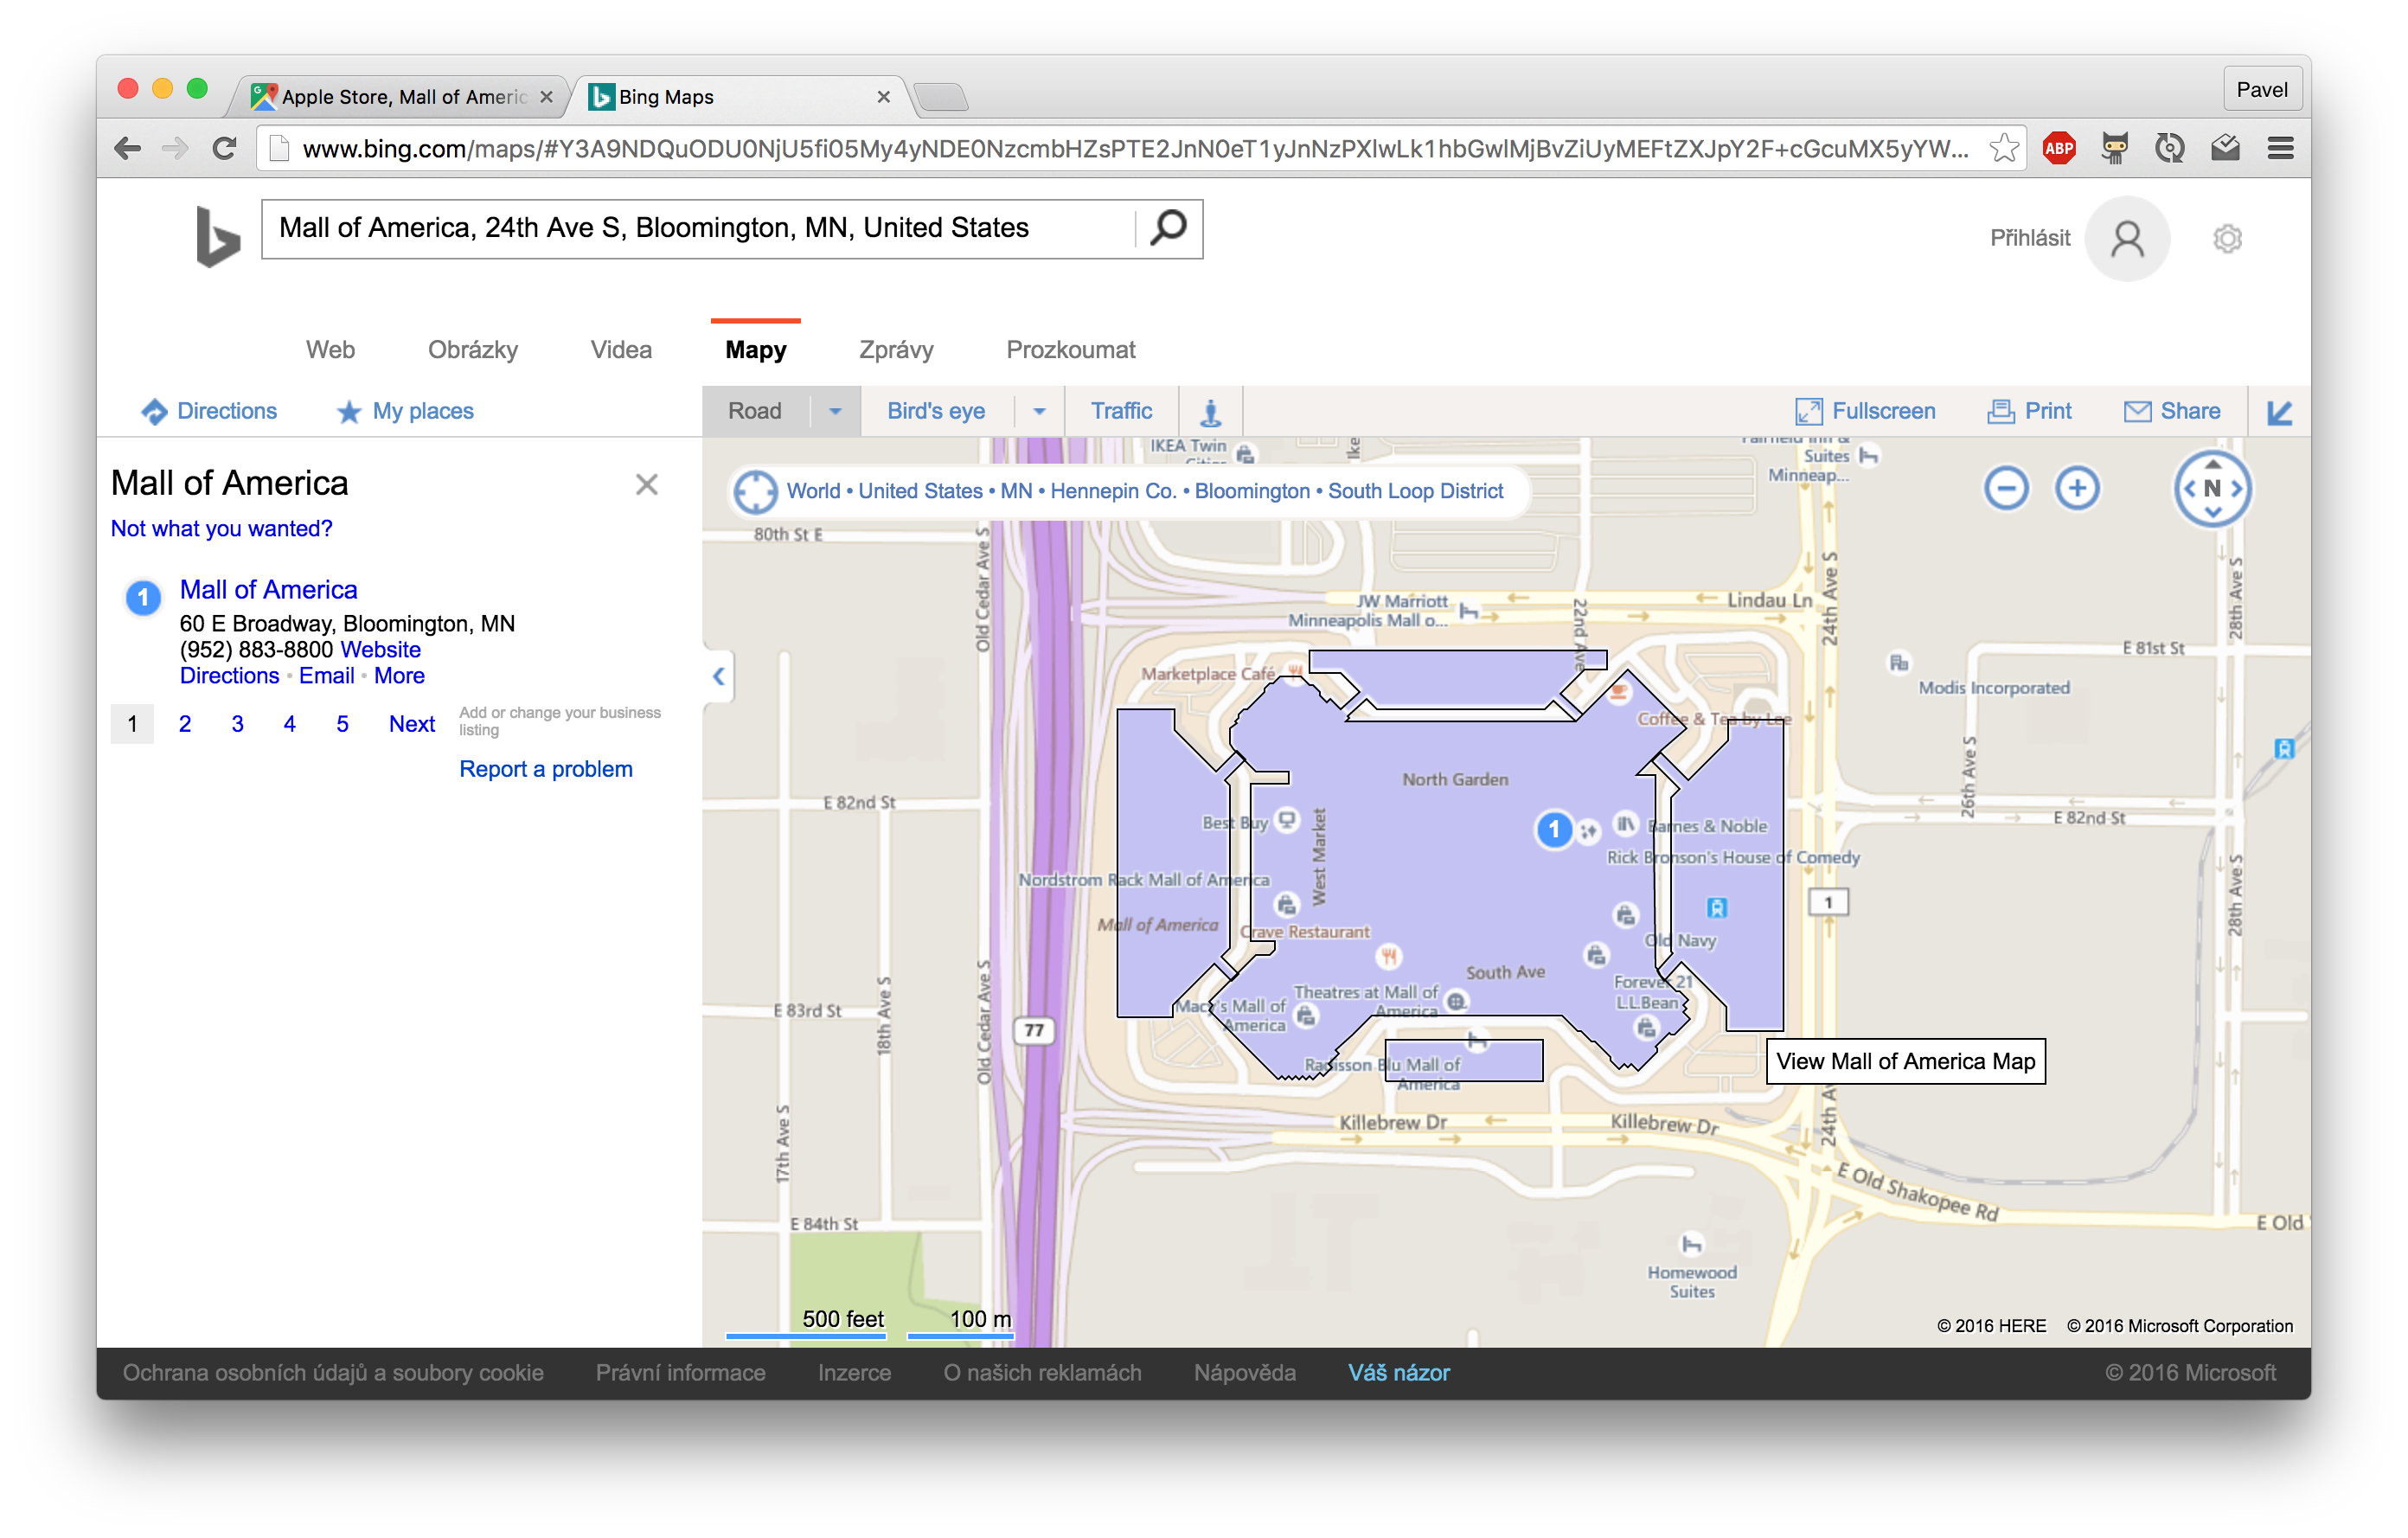
\includegraphics[width=.5\linewidth]{img/4a-bing-moa-1.png}}\hfill
                    \subfloat[\label{obr4b}]
                    {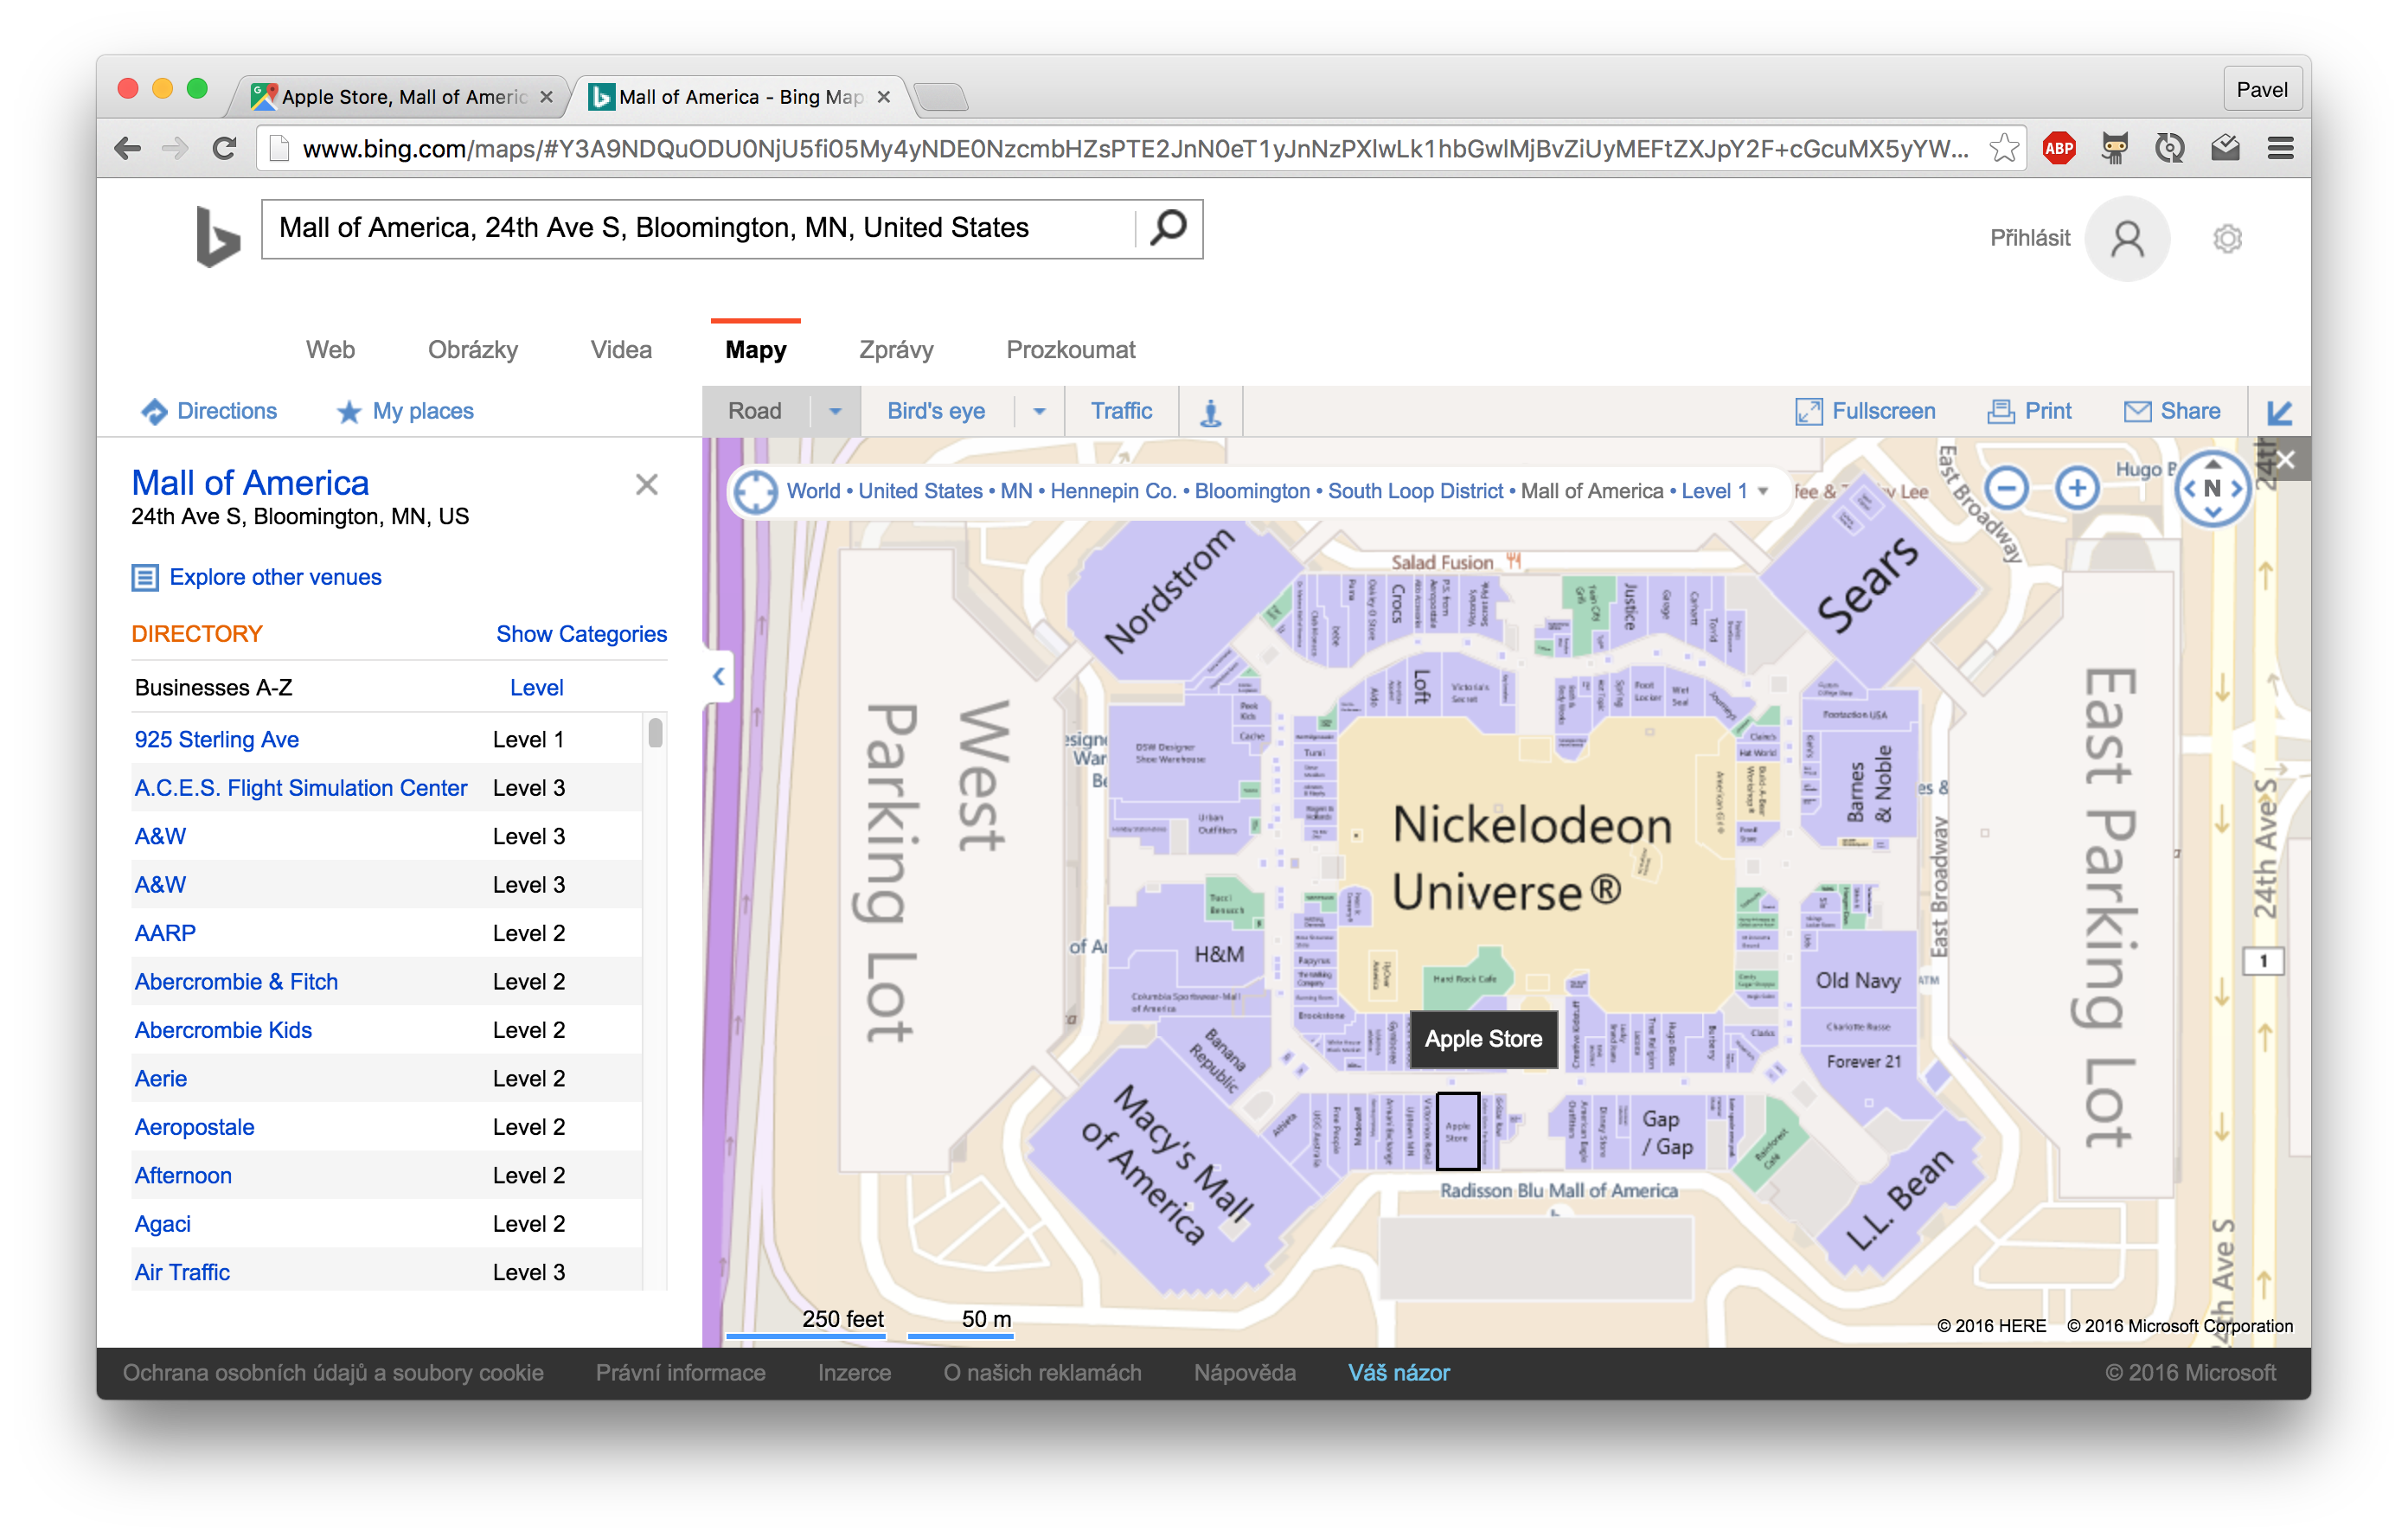
\includegraphics[width=.5\linewidth]{img/4b-bing-moa-1-indoor.png}}\hfill
                    \subfloat[\label{obr4c}]
                    {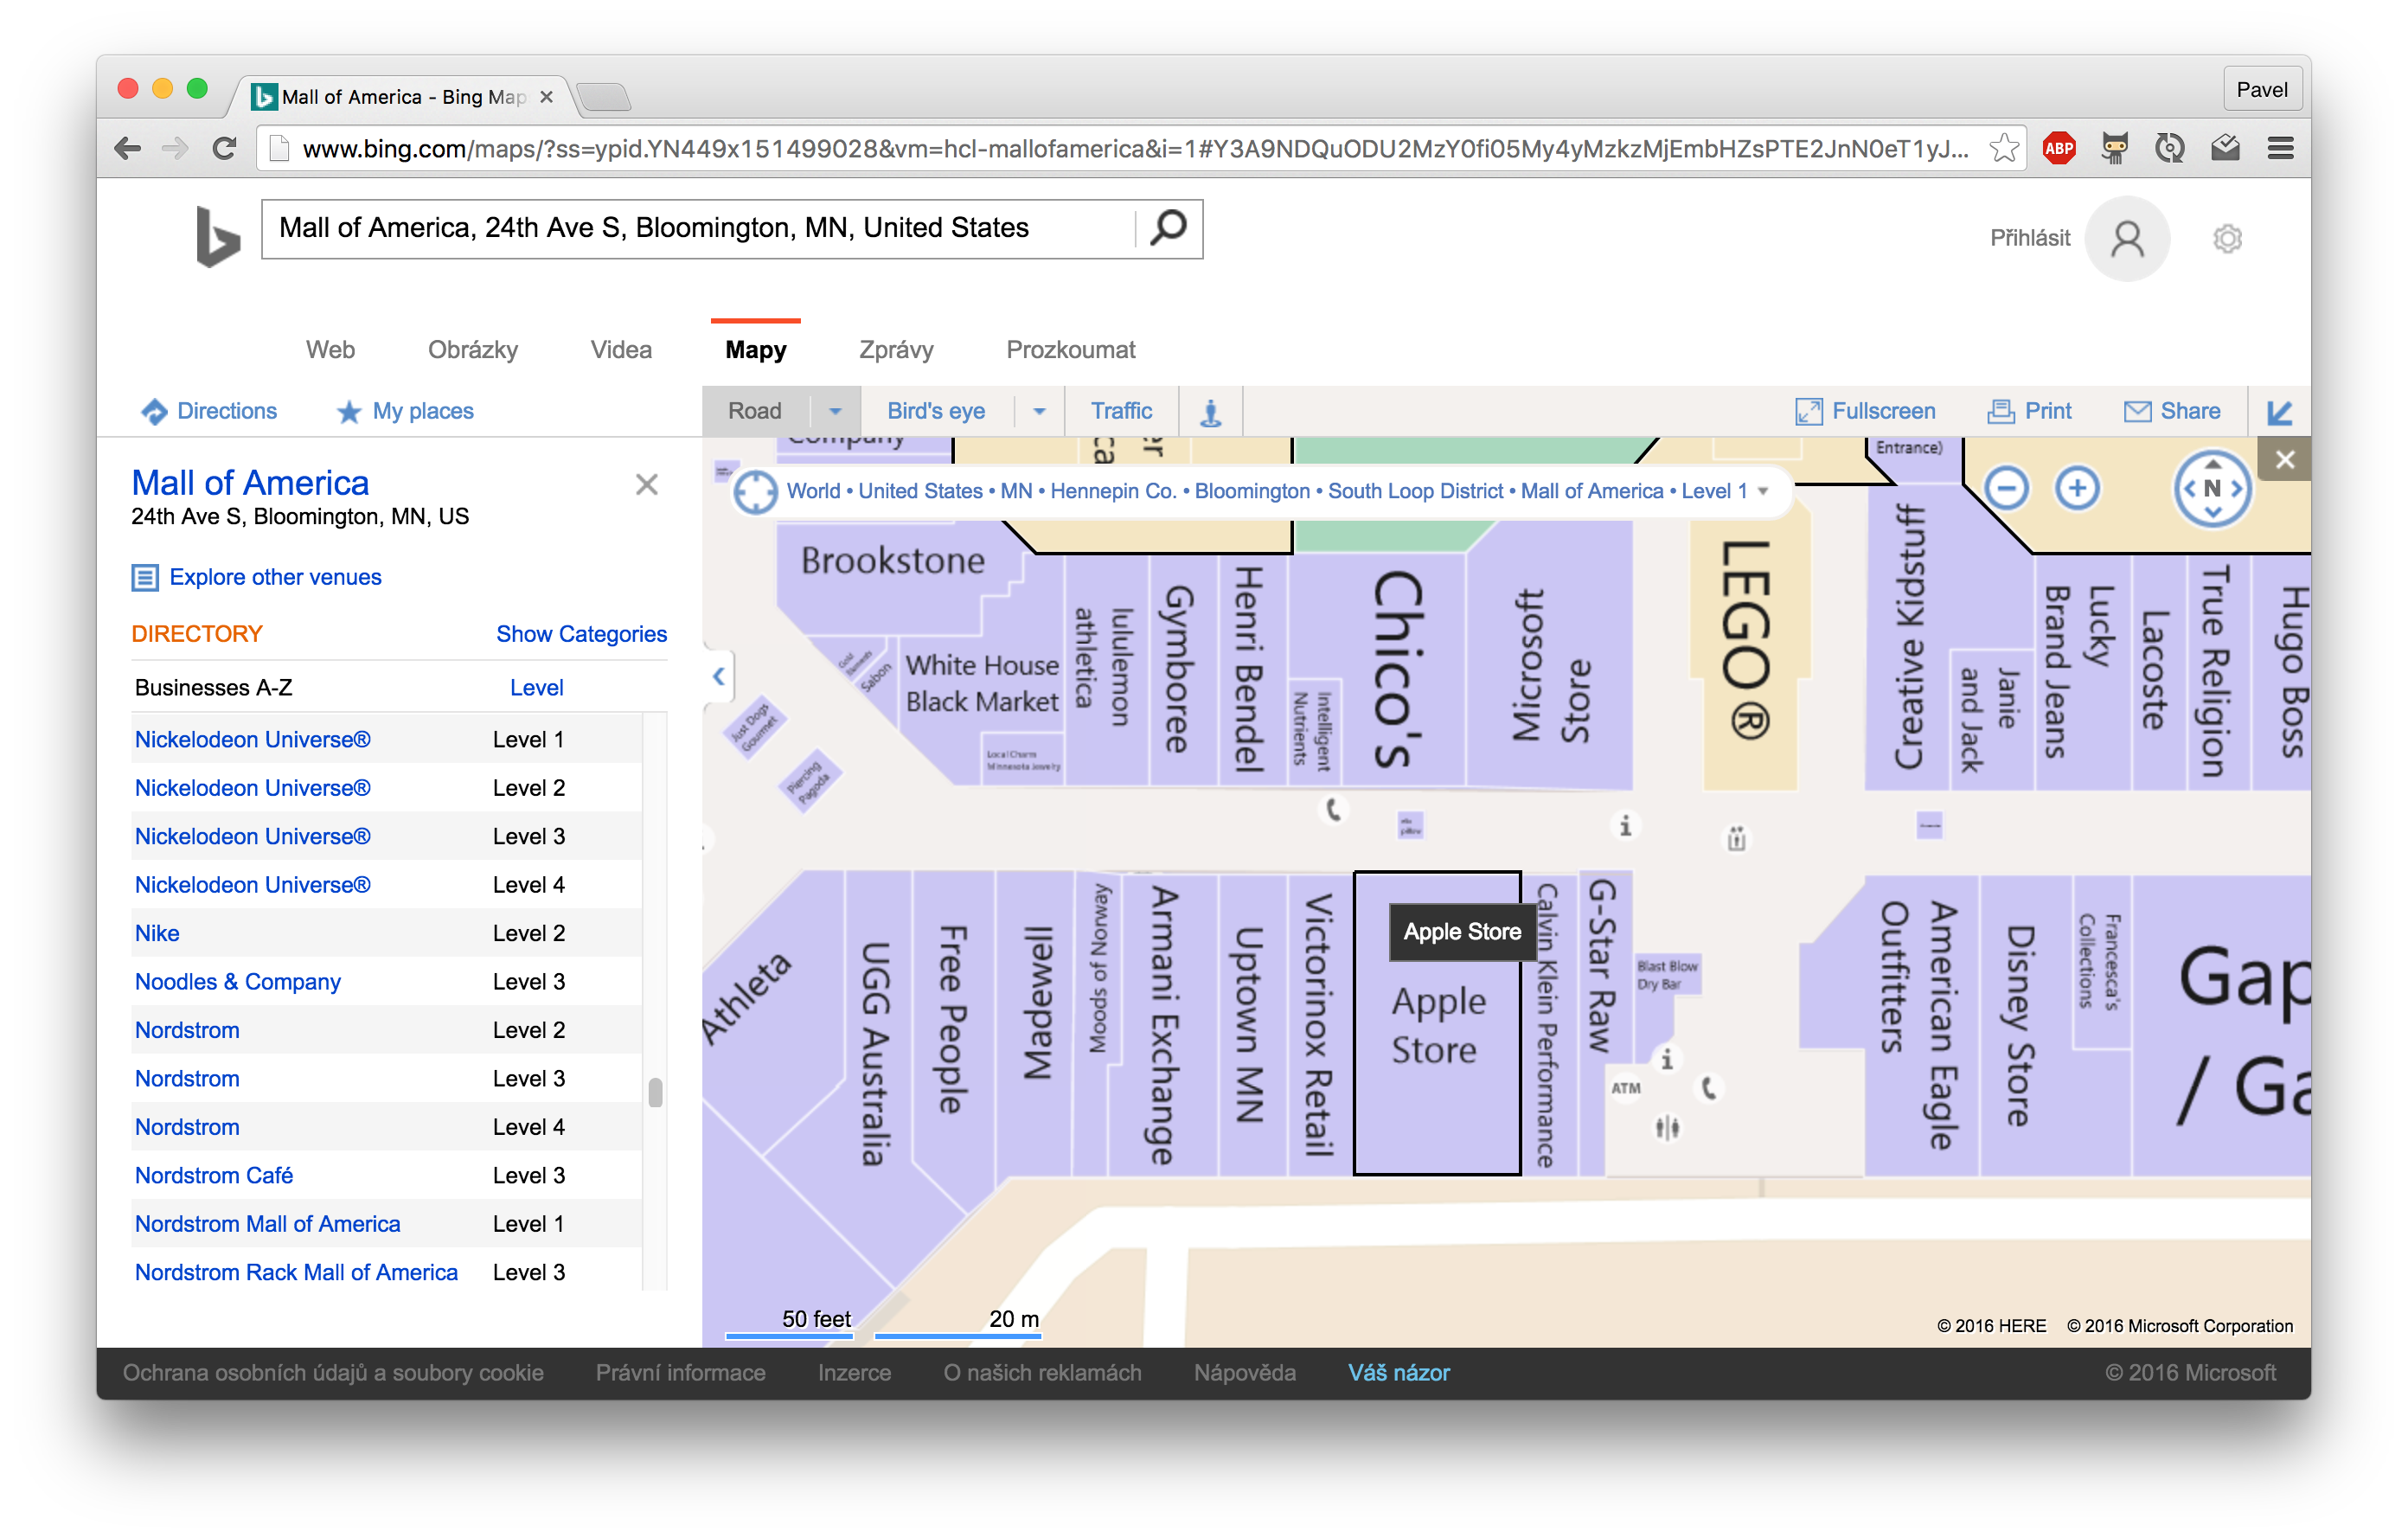
\includegraphics[width=.5\linewidth]{img/4c-bing-moa-2.png}}

                    \caption{Zobrazení klasické mapy~v~Bing Maps (a); přepnutí do indoor zobrazení (b); přiblížení (c)}
                    \label{obr4}
                    \end{figure}
                    

Společnost Microsoft spustila své webové mapy původně pod názvem Microsoft Virtual Earth na konci roku 2005. Přestože v~množství vlastností dostihuje Google Maps (letecké pohledy, street view, 3D mapy, dopravní informace), stále zůstává několik kroků za ním. Chybí například podpora pro jiné mobilní platformy než Windows Phone. Pokrytí leteckých map či street view je subjektivně horší.

Své indoor řešení pod názvem Bing Venue Maps spustila v~roce 2011. Zobrazení je podobné službě Micello, a tedy subjektivně přehlednější než Google. Obsahuje 5~400~míst. Indoor režim se aktivuje kliknutím na zvýrazněnou budovu, přepínač pater je umístěn do drobečkové navigace v~rámci mapy (dle mého mírně schovaný). Služba navíc nabízí adresář~business listingů~v~budově a též možnost procházet Venue Maps podle země a kategorie. Pro ČR eviduje 2 letiště, 45 nákupních center a pražskou zoologickou zahradu.

Služba vypadá z~dnešního pohledu mírně zastarale, Microsoft totiž posledních několik let vyvíjí tzv. Bing Maps Preview, které ovšem lze nainstalovat pouze jako~aplikaci pro Windows 10.

\subsection{Micello}\label{micello}

Společnost Micello se označuje za vedoucího poskytovatele indoor map. Nabízí přes 25 000 zmapovaných míst,\cite{zdroj21}~v~ČR je to asi desítka míst se subjektivně menší úrovní detailů než Bing. Společnost se specializuje zejména na prodej dat, vlastní aplikace nevyvíjí. Na jejím webu lze najít jen omezený prohlížeč.

Aktivace indoor se provádí kliknutím na ikonku budovy, chybí přímá integrace do okolní mapy. Ikonky jsou v~tomto případě zobrazeny na API Google Maps. Na začátku roku 2016 oznámila spolupráci se startupem eeGeo, jehož cílem je zmapovat celou Zemi ve 3D.\cite{zdroj22}

Jako jediný z~komerčních projektů umožňuje omezenou editaci veřejností. Uživatel může zadat až 3 poznámky (návrhy na přejmenování, rozdělení prostor apod.), které pak Micello projde a případně schválí. Dále jako jediný disponuje indoor routováním.

Ukázka dostupná na: \href{http://www.micello.com/coverage}{www.micello.com/coverage}~


                      \begin{figure}
                    	  \centering
                    \subfloat[\label{obr5a}]
                    {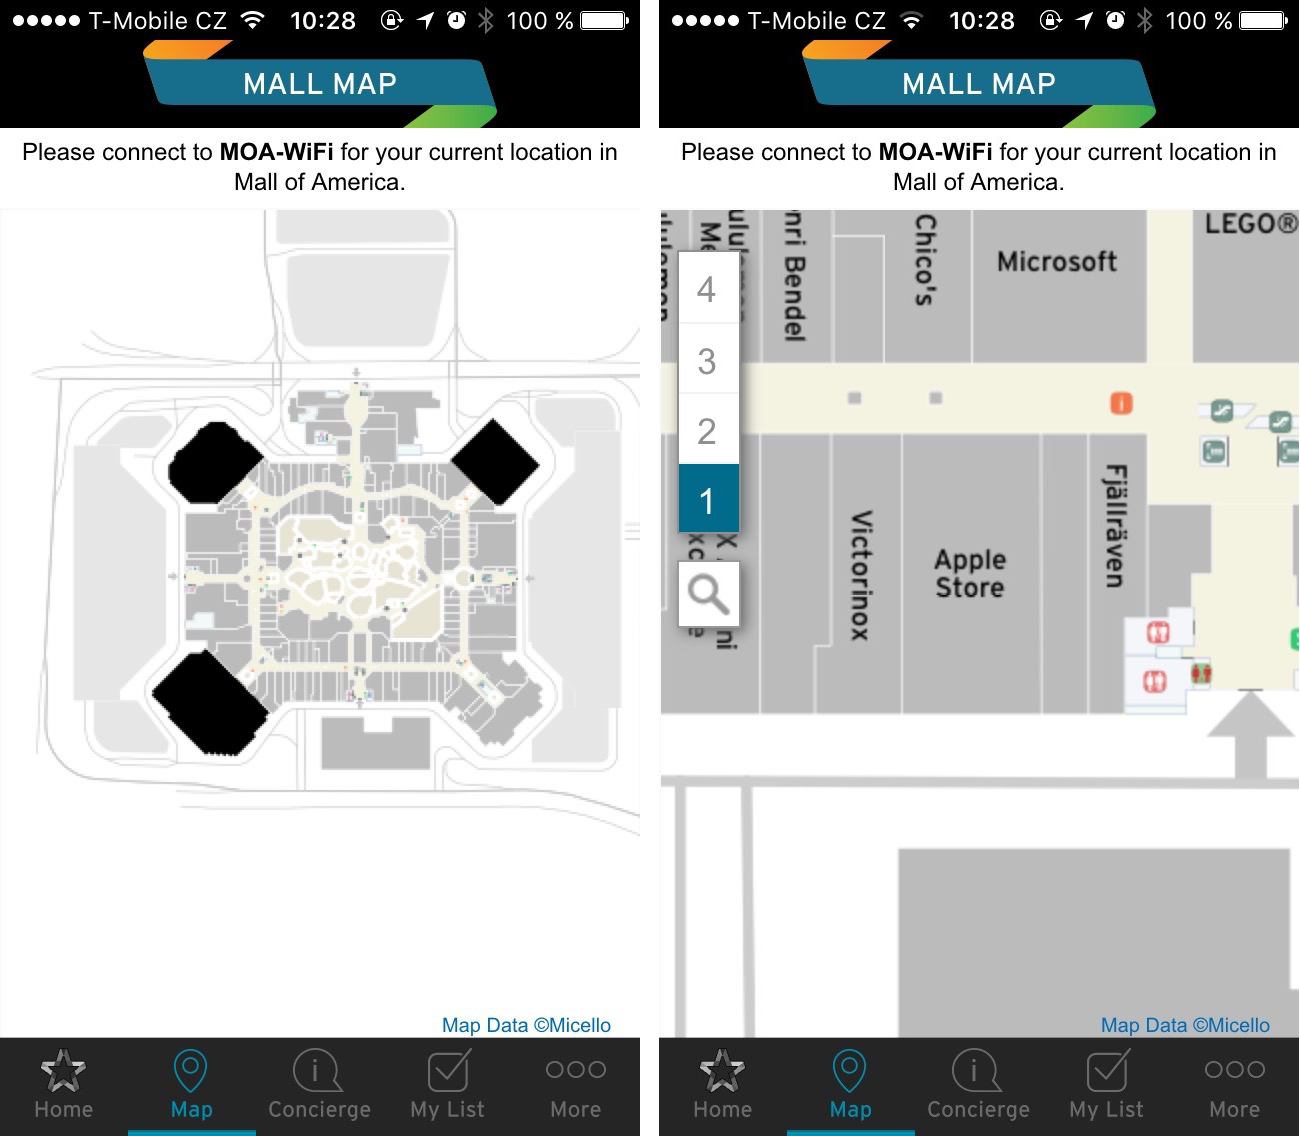
\includegraphics[width=.6\linewidth]{img/5a-micello1i2.png}}\hfill
                    \subfloat[\label{obr5b}]
                    {\includegraphics[width=.5\linewidth]{img/5b-micellob0.png}}\hfill
                    \subfloat[\label{obr5c}]
                    {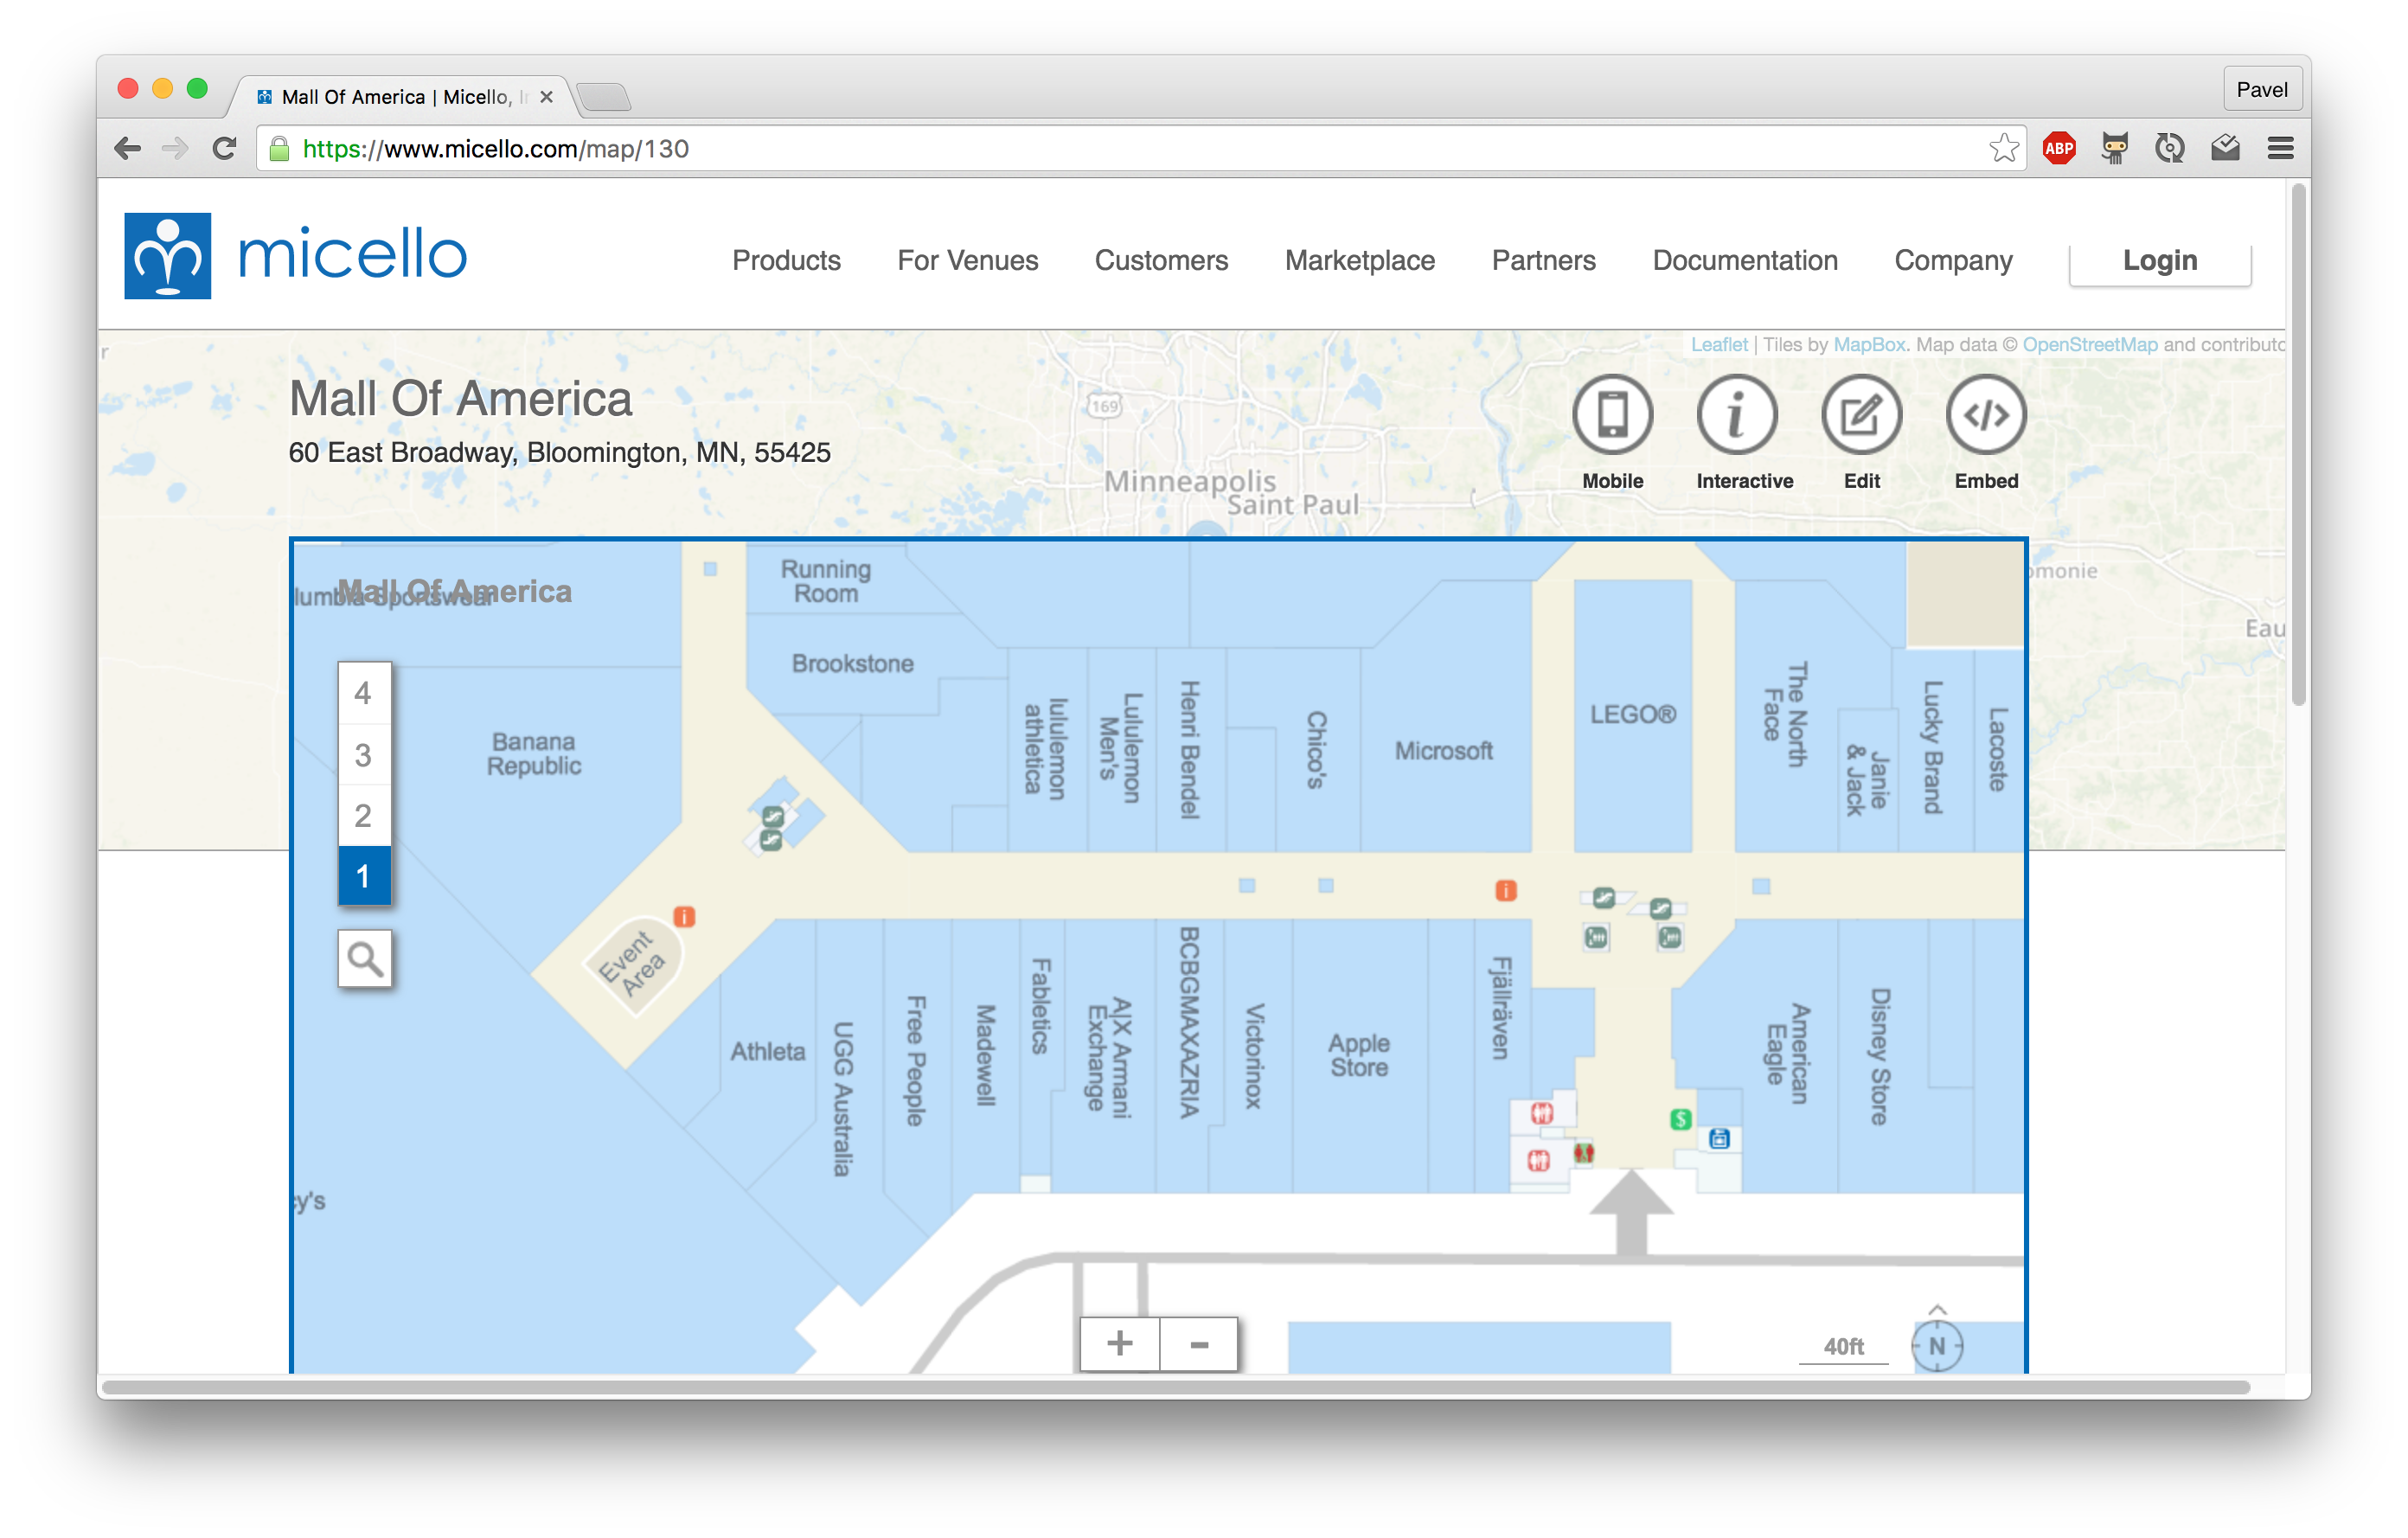
\includegraphics[width=.5\linewidth]{img/5c-micellob1.png}}

                    \caption{Implementace indoor prohlížeče v~aplikaci \uv{Mall of America} (a); Ukázka pokrytí (b) a prohlížeče (c) na webu Micello\cite{zdroj23}}
                    \label{obr5}
                    \end{figure}
                    

\subsection{Open-source platforma Anyplace}\label{open-source-platforma-anyplace}

Otevřená platforma pod licencí MIT nabízí kompletní řešení pro indoor tvorbu, prohlížení i geolokaci a klientské aplikace pro všechny velké mobilní platformy.\cite{zdroj24} Zdrojové kódy jsou dostupné na GitHubu, včetně nástroje pro zaměření zemského pole kompasem. Vývoj provádí skupina na University of Cyprus. Díky open-source povaze celého projektu se na něj můžeme podívat blíže, zejména s~ohledem na možné využití některých komponent pro budoucí řešení nad platformou OpenStreetMap.


                      \begin{figure}
                    	  \centering
                    \subfloat[\label{obr6a}]
                    {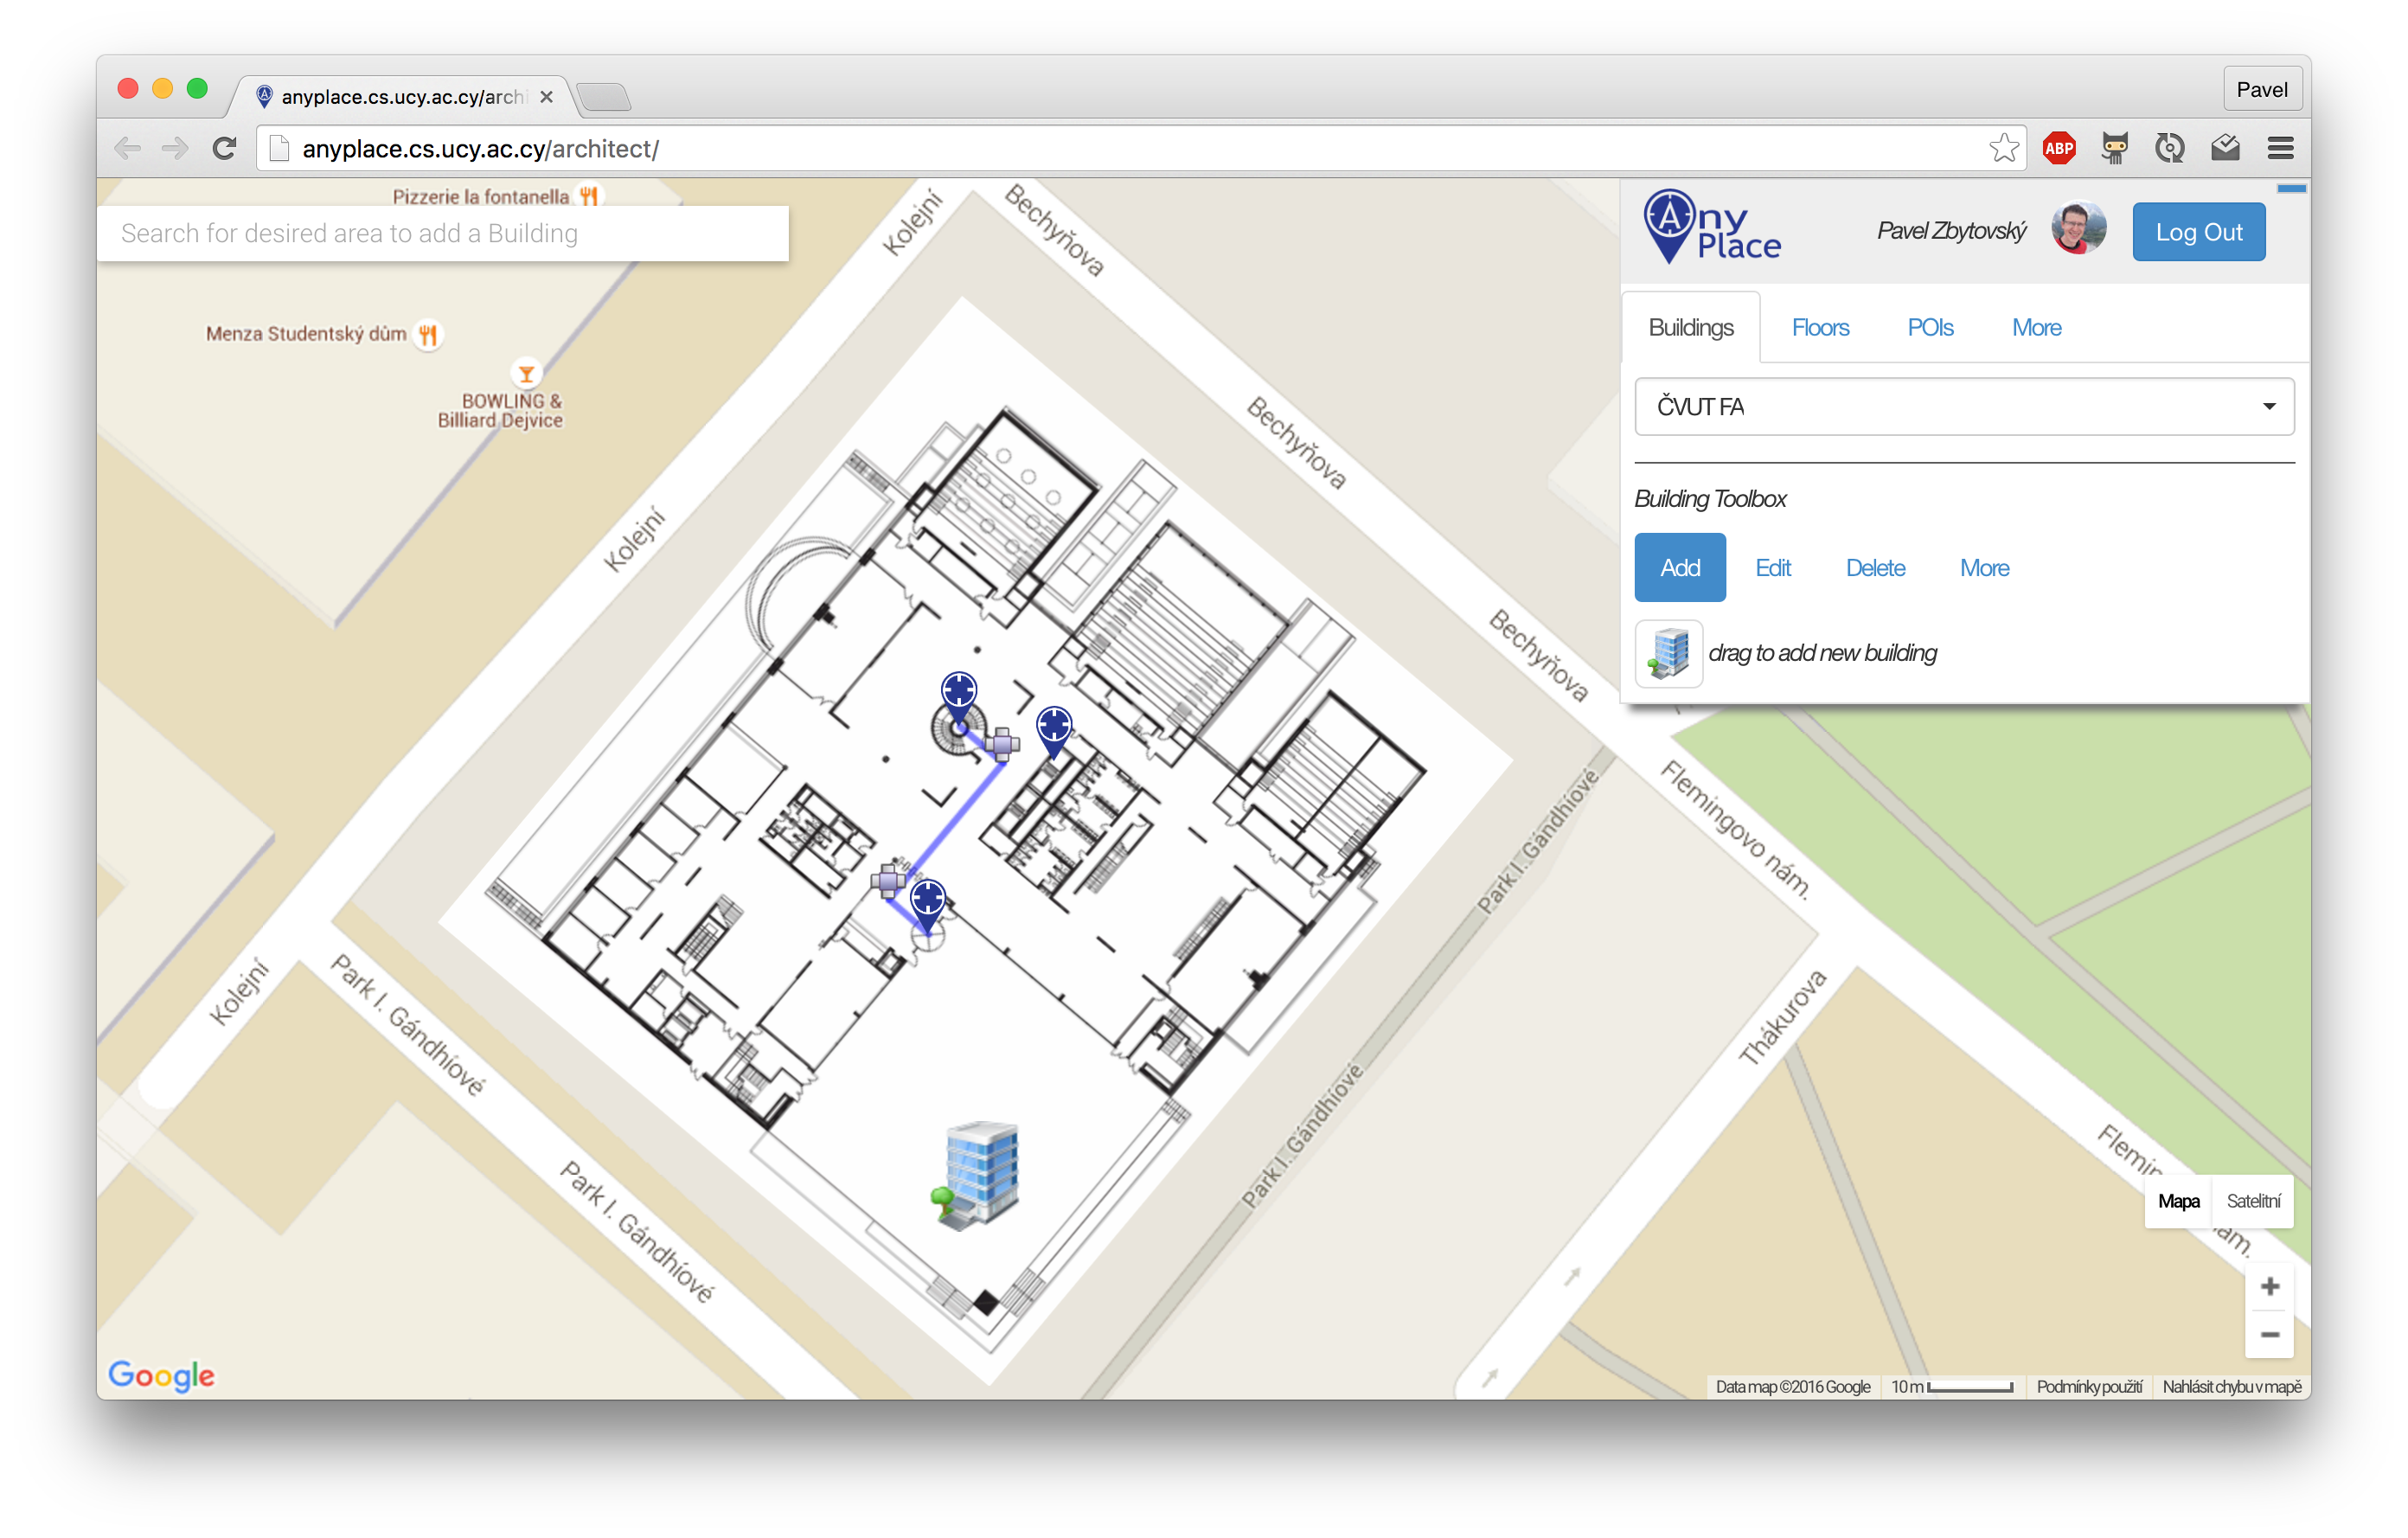
\includegraphics[width=.5\linewidth]{img/6a-anyplace-webeditor.png}}\hfill
                    \subfloat[\label{obr6b}]
                    {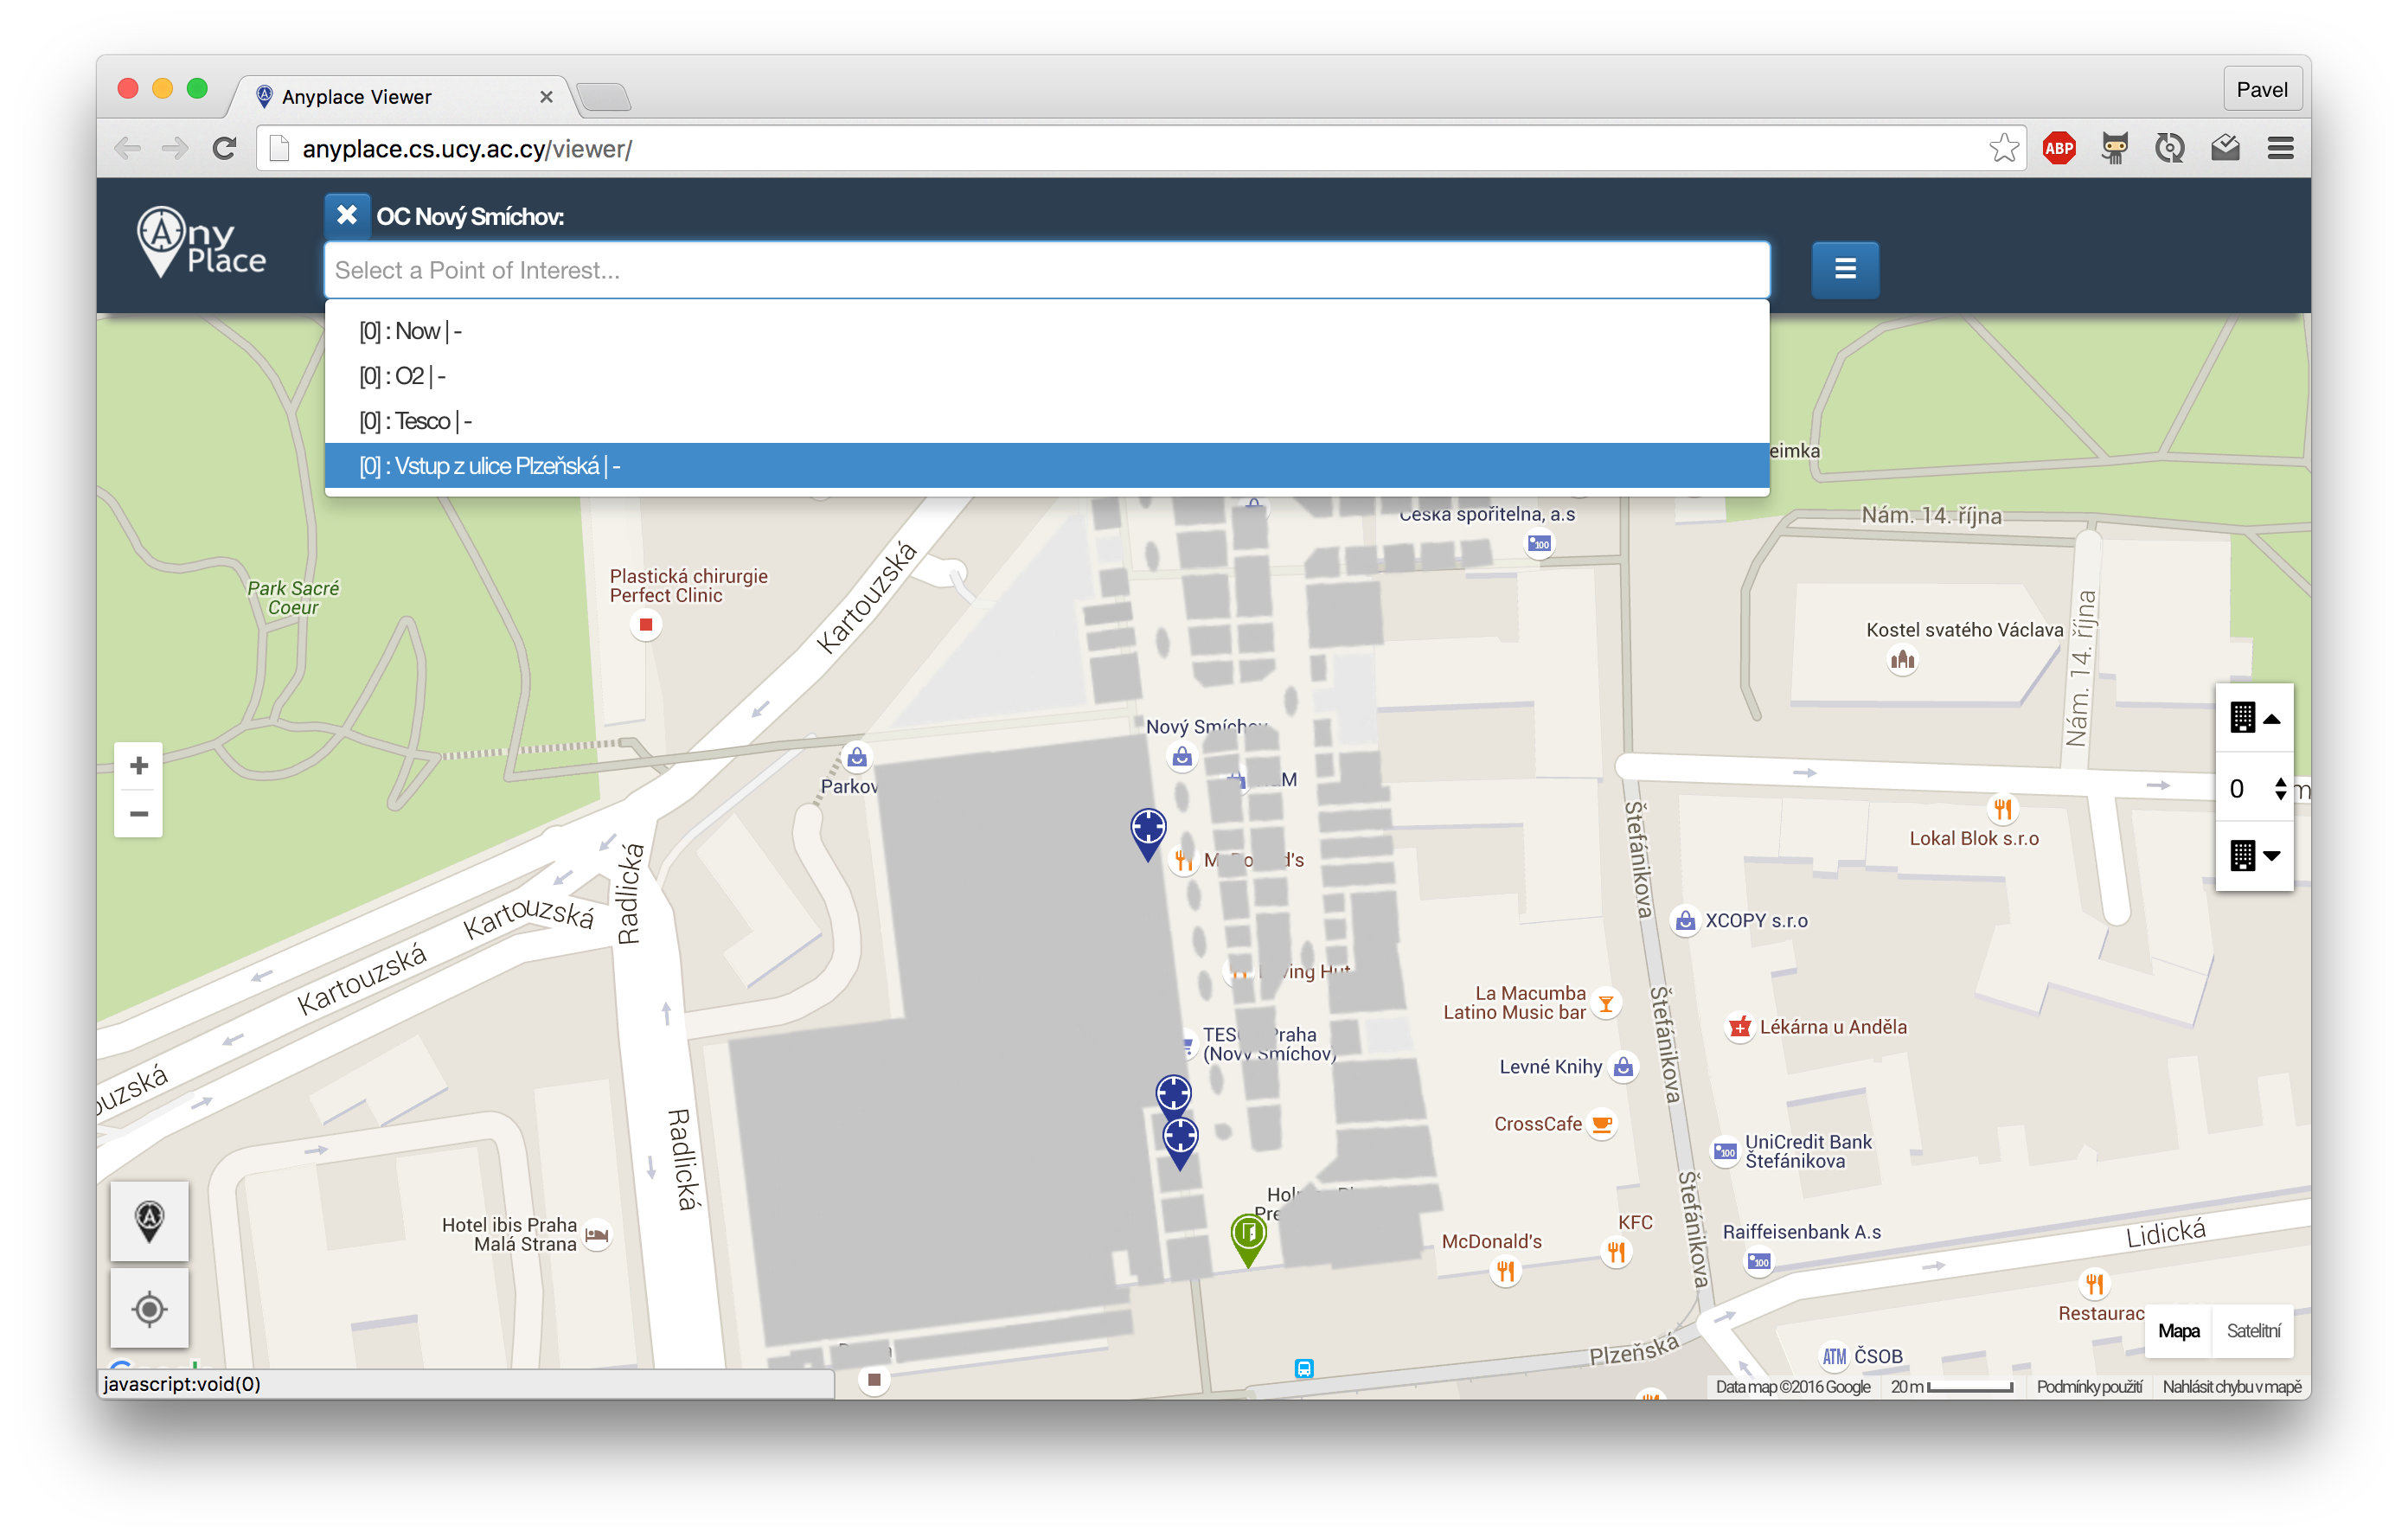
\includegraphics[width=.5\linewidth]{img/6b-anyplace-viewer-andel.png}}\hfill
                    \subfloat[\label{obr6c}]
                    {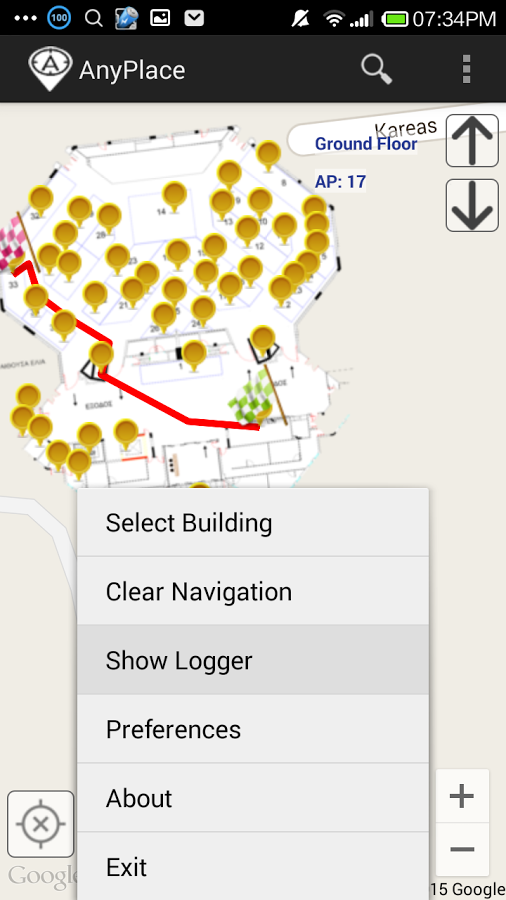
\includegraphics[width=.3\linewidth]{img/6c-anyplace-logger.png}}

                    \caption{Editace plánu FA ČVUT (a); zobrazení plánu OC Smíchov (b); logger pro Android (c)\cite{zdroj25}}
                    \label{obr6}
                    \end{figure}
                    

Do Anyplace může po přihlášení kdokoliv nahrát podlažní plán své budovy. Ten je třeba přesně zarovnat nad zobrazenou Google mapou a následně je možné podlaží pojmenovat, přidat body zájmu a též vytvořit routovací graf (\uv{Add new edge}). Zarovnání podlaží je však subjektivně velmi nepříjemné a není ani dobře možné přidat vyšší podlaží na stejné místo.

Zobrazovací rozhraní Anyplace je implementováno také nad API Google Maps. Podobně jako v~Micello jsou v~klasické mapě ikonky zmapovaných budov, ovšem po rozkliku se budova v~mapě jen elegantně překryje zvoleným plánem podlaží. Umožňuje prohledání všech bodů zájmu, jednoduché zobrazení trasy mezi body a možnost sdílet adresu či vložit mapku do jiného webu.

Celá aplikace včetně editace je postavena nad vlastním RESTful API, které je i dobře dokumentováno.\cite{zdroj26}~Nabízí se tak například i teoretická možnost importu-exportu dat mezi Anyplace a OpenStreetMap.

Mobilní aplikace pro platformy Android a Windows Phone jsou spíše proof-of-concept, ale nabízejí alespoň~základní funkcionalitu. Android aplikaci lze přepnout též do režimu Logger, kdy zaznamenává data pro indoor geolokaci na základě Wi-Fi, kompasu a IMU~(viz. kapitola 1.2).

Anyplace se tedy jeví jako velmi vhodný zdroj pro další využítí, zejména v~kombinaci s~indoor daty OpenStreetMap.

Více informací na \href{http://github.com/dmsl/anyplace}{github.com/dmsl/anyplace}~

\subsection{Codrops Interactive 3D Mall Map}\label{codrops-interactive-3d-mall-map}

Tento koncept moderního prohlížeče indoor plánu nákupního centra je vytvořen pomocí technologií CSS a SVG. Projekt je k~dispozici jako open-source na GitHubu, zveřejněný pod licencí podobnou CC-BY-SA.

Sice nejde o~mapovou aplikaci, ale i tak nabízí zajímavou inspiraci z~hlediska interakčního designu (UX). Možné využíti je diskutováno v~kapitole 4.

Více informací na \href{http://github.com/codrops/Interactive3DMallMap}{github.com/codrops/Interactive3DMallMap}


                      \begin{figure}
                    
                    \subfloat[\label{obr7a}]
                    {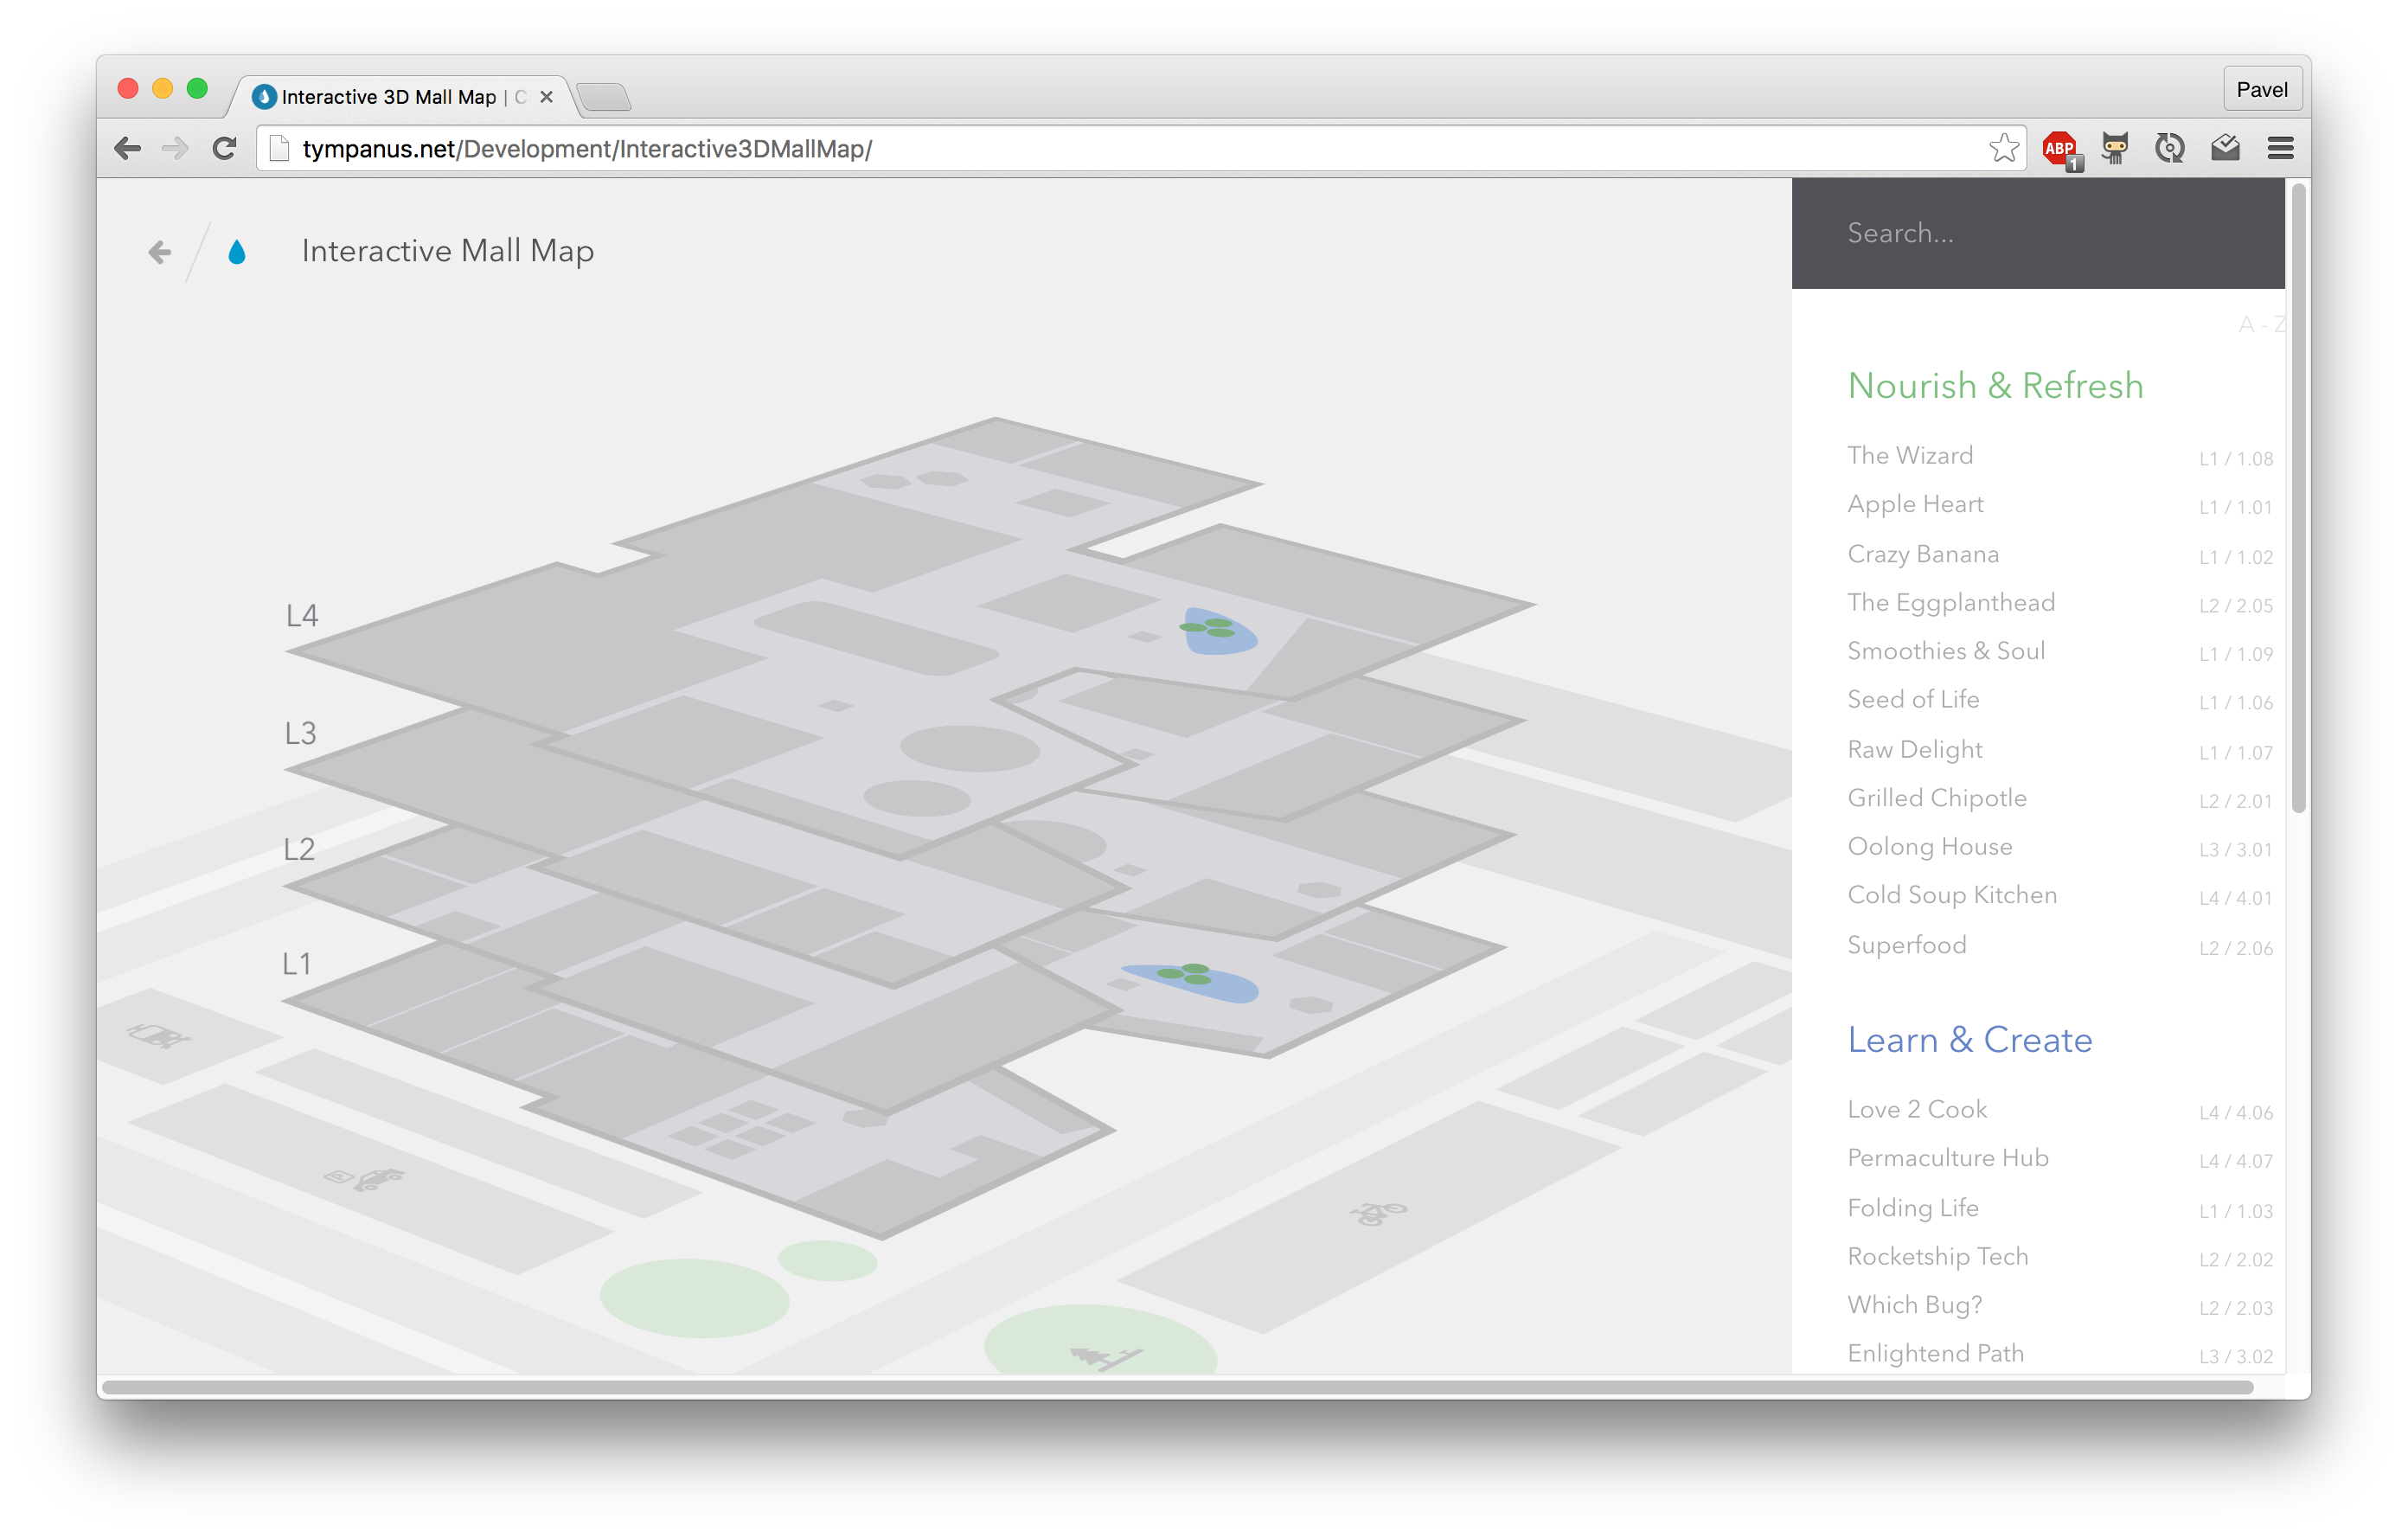
\includegraphics[width=.5\linewidth]{img/7a-codrops-3d.png}}\hfill
                    \subfloat[\label{obr7b}]
                    {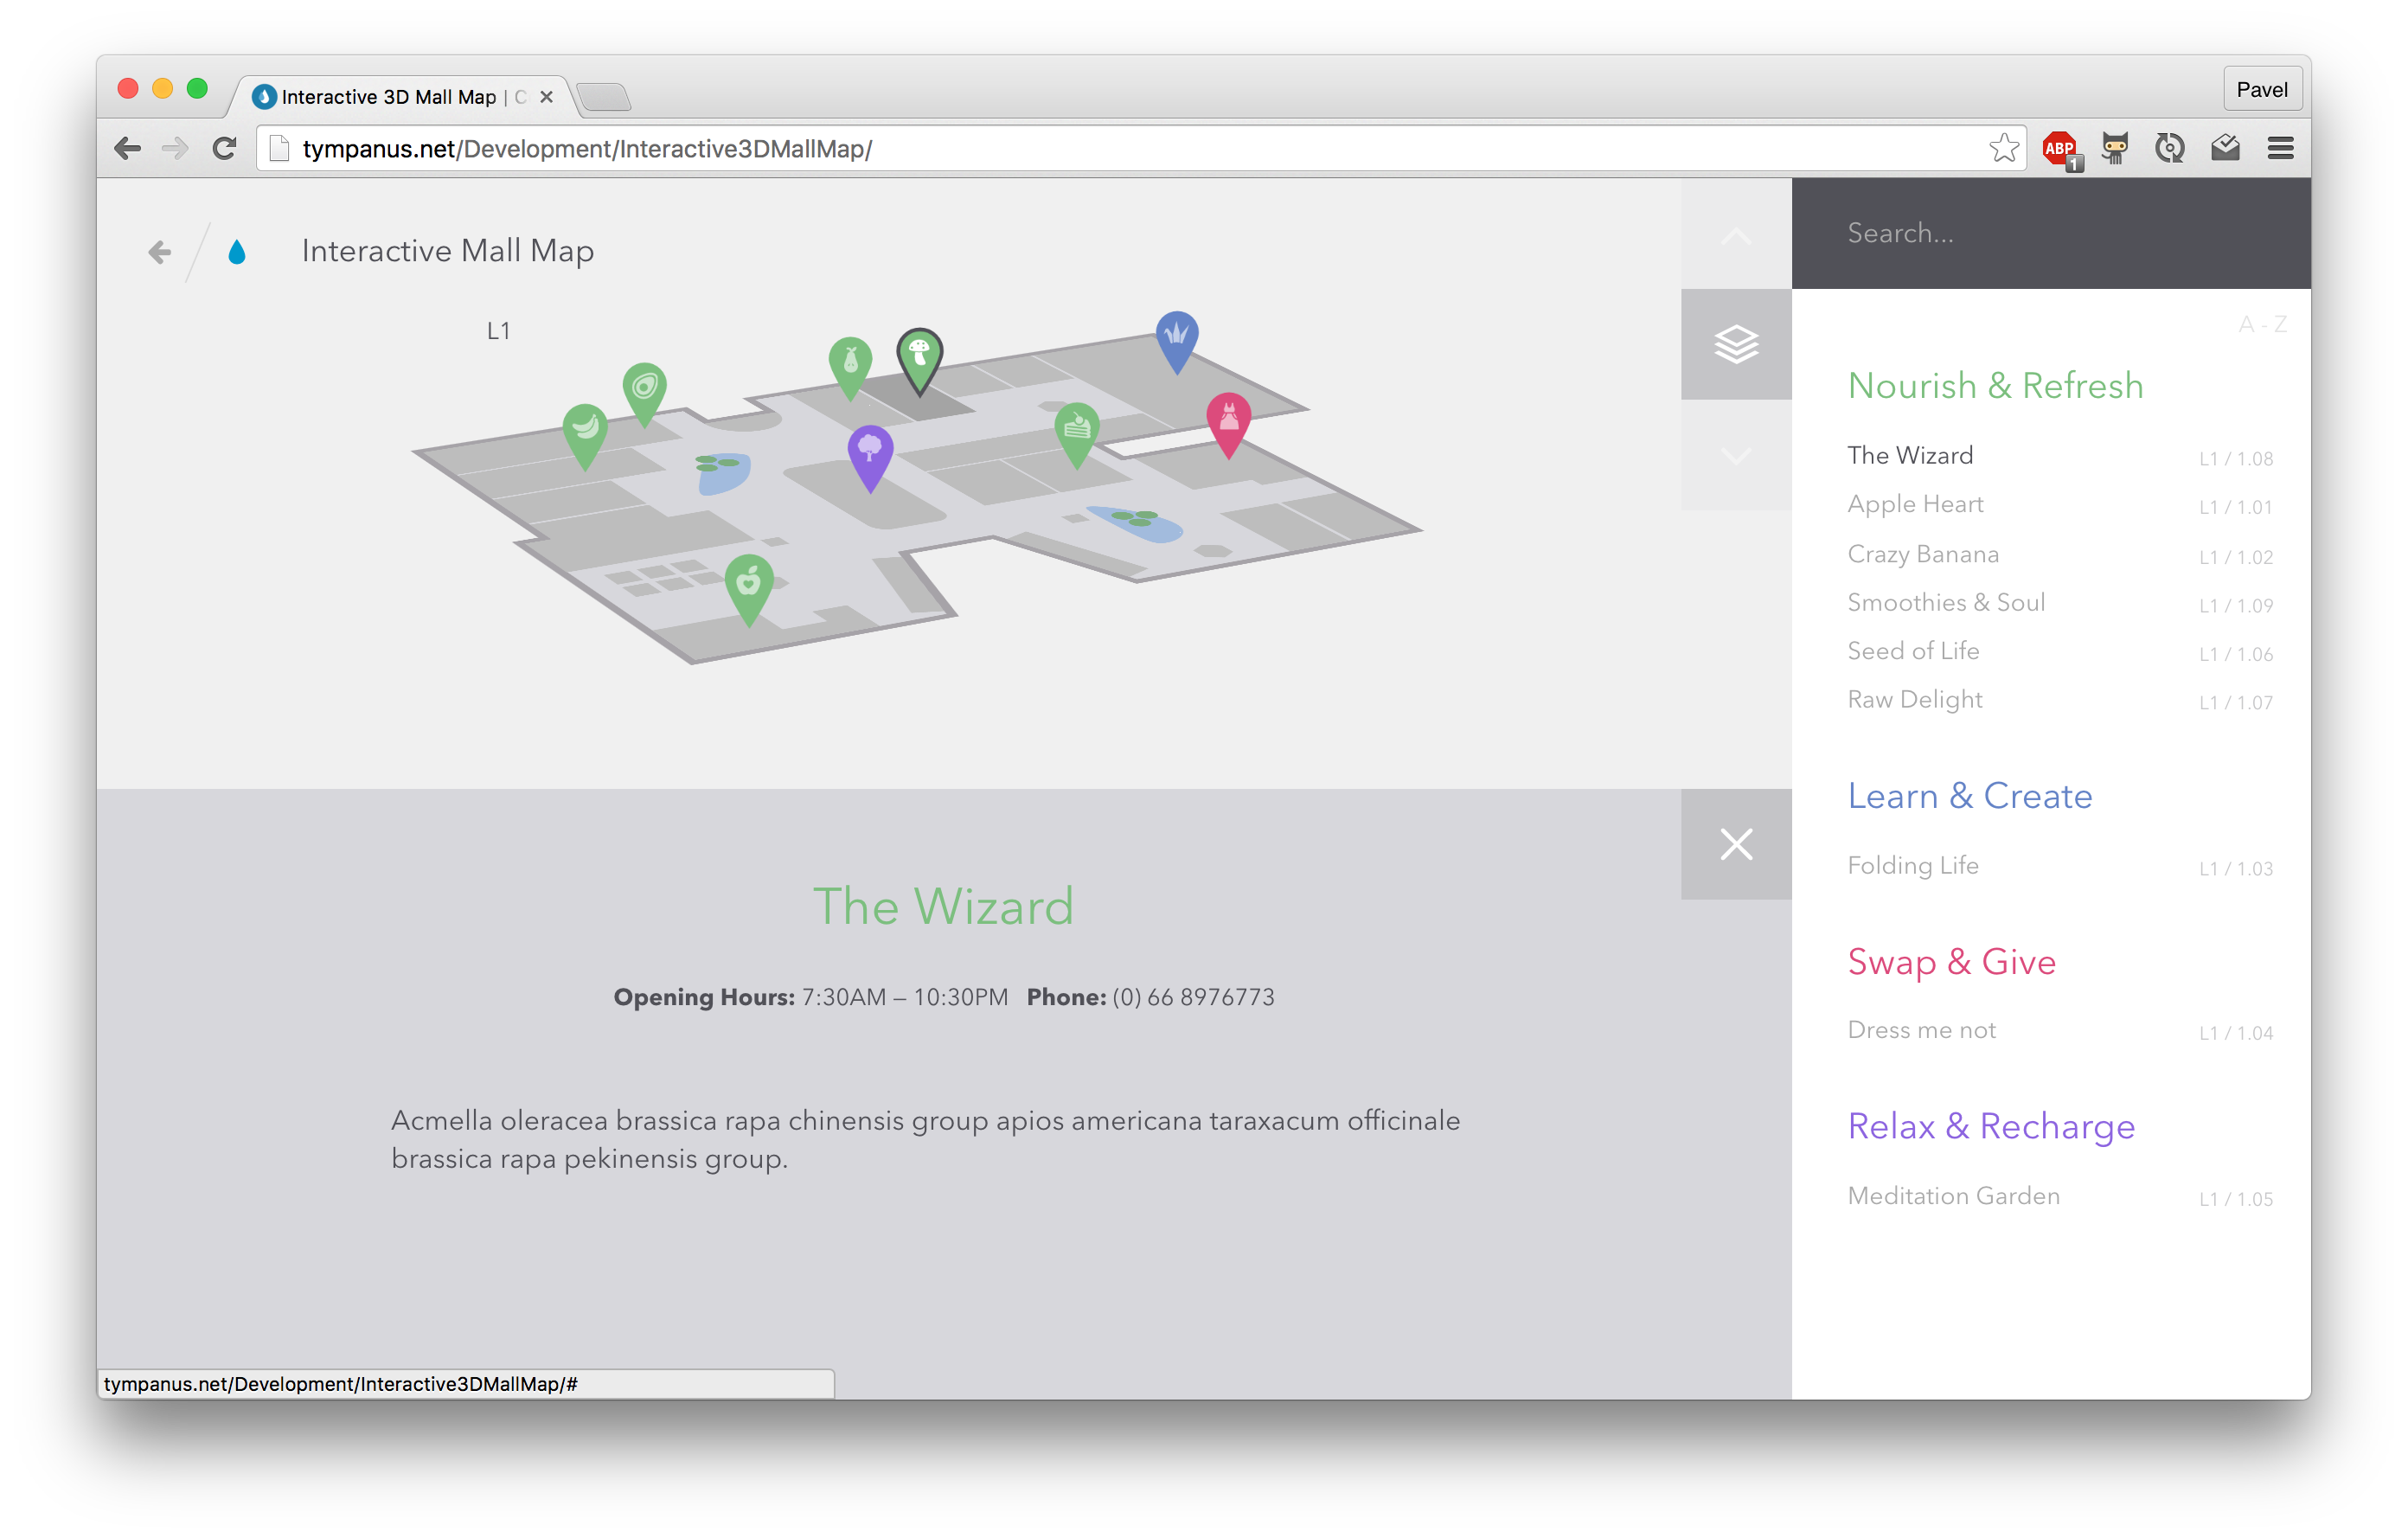
\includegraphics[width=.5\linewidth]{img/7b-codrops-2.png}}

                    \caption{Vizualizace pater nákupního centra v~Codrops}
                    \label{obr7}
                    \end{figure}
                    

\subsection{ČVUT Navigátor}\label{ux10dvut-naviguxe1tor}

Před několika lety vytvořili kolegové z~ČVUT platformu pro správu a zobrazení indoor map, zejména pro navigaci.\cite{zdroj27}~V~současné době není v~provozu, ale jednu z~výsledných~mobilních~aplikací~pěkně prezentuje video dostupné na YouTube\footnote{\href{https://www.youtube.com/watch?v=3xEbvc49mgQ}{www.youtube.com/watch?v=3xEbvc49mgQ}}~-- zahrnovala rozvrh studenta, klasickou městskou mapu pro vyhledání budovy, navigační indoor mapy a geolokaci pomocí QR kódů~zpestřenou tzv. rozšířenou realitou.

Plány jednotlivých podlaží byly rastrové a nad nimi byl ručně vytvořen routovací graf. Datovým zdrojem byla serverová aplikace nad speciálně navrženým API. Tvorba a úprava plánů~byla umožněna~všem členům akademické obce. To byl i hlavní důvod vzniku tohoto projektu, protože předchozí podobné pokusy selhaly na tom, že je nikdo neudržoval.

Tento rok~(2016) bude též obhajováno několik závěrečných prací pod názvem ČVUT Navigátor 3.0. Soustředí se na různé klientské aplikace pro indoor navigaci. Využívají nové vektorové API nad CMS ModX. \footnote{Naše práce řeší obecný problém získávání a správy indoor map v~rámci otevřené, zavedené platformy OpenStreetMap, může tedy být v~budoucnu zdrojem i pro toto ~navigační řešení. }

\subsection{i-locate consorcium a IndoorGML formát}\label{i-locate-consorcium-a-indoorgml-formuxe1t}

V~souvislosti s~touto prací je třeba zmínit program podpořený Evropskou unií, který si klade za cíl~vytvořit \uv{protějšek OpenStreetMap pro indoor použití}.\cite{zdroj28}~Projekt běží od začátku roku 2014 do konce 2016 a měl by vytvořit infrastrukturu, nástroje a formáty pro open-data i crowd-sourcing.

Důležitou částí projektu je IndoorGML formát -- standard přijatý OpenGeo Consorciem.\cite{zdroj29}~Měl by sloužit jako otevřený XML~formát pro výměnu a modelování indoor dat, včetně možnosti pro využití routingu a napojení na na struktury vnějšího světa, tedy například formát CityGML. Editor IndoorGML je postaven jako plugin\cite{zdroj30}~editoru JOSM (více v~kapitole 2.2.).

\subsection{Google Project Tango}\label{google-project-tango}

Google se již delší dobu zabývá přesným modelováním prostoru, trasování polohy a vnímání hloubky.\cite{zdroj31}~Připravuje tak půdu pokročilým aplikacím rozšířené reality\footnote{Obraz reálného světa je doplněn objekty generovanými počítačem, anglicky Augmented Reality}, ale počítá se i s~crowd-sourcingem vnitřních prostorů pro mapy. V~únoru 2016 Google nabídl~působivé demo\cite{zdroj32}, ve kterém tablet při procházení muzeem živě modeluje okolní 3D prostor, zná svou polohu s~přesností na centimetry a díky tomu ukazuje v~rozšířené realitě navigační prvky na podlaze. Tento systém sice vyžaduje speciální podporu hardwaru (přesnější senzory, kamery, výkon atd.), ale velmi dobře ilustruje, kam by se mohla technologie indoor geolokace a navigace ubírat.

 \begin{figure}
	  \centering
      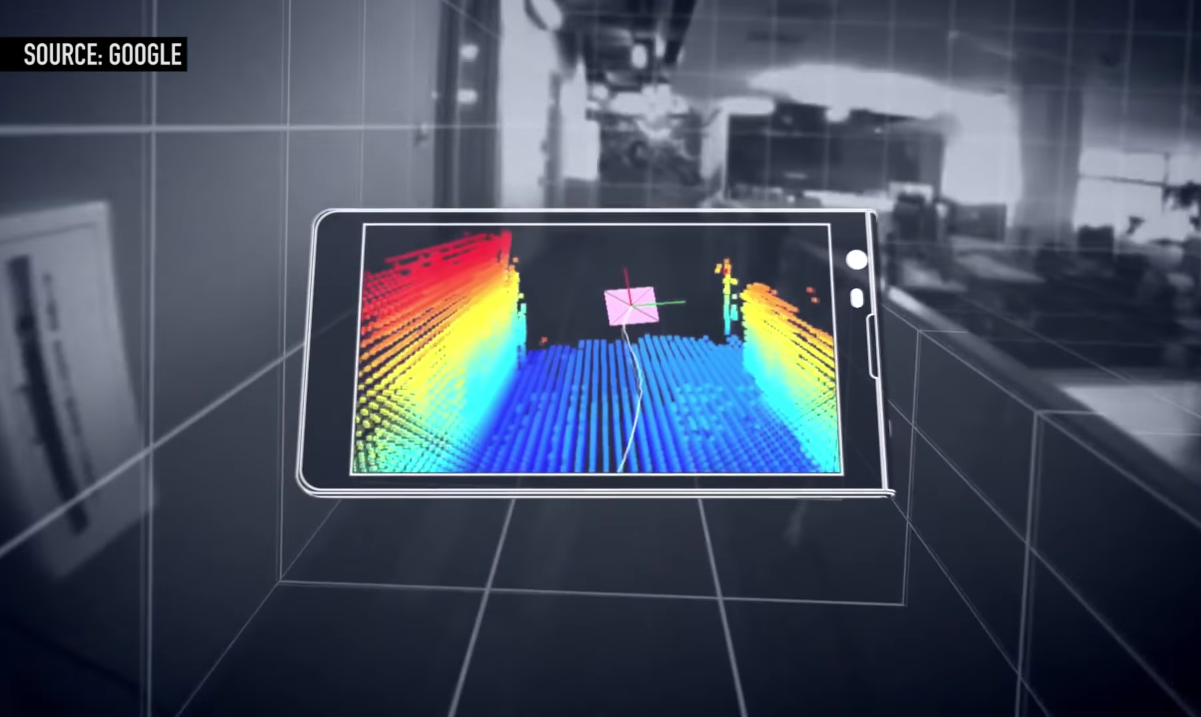
\includegraphics[width=\textwidth]{img/8-google-tango.png}
      \caption{Ilustrační obrázek rozpoznáného 3D profilu a zaznamenané stopy}
      \label{obr8}
  \end{figure}

\section{Geolokace}\label{geolokace}

Pro venkovní použití se nejčastěji mluví o~satelitní navigaci~-- tedy dopočítání polohy triangulací z~obdržených časových razítek několika satelitů. Pro určení polohy (tzv. fix) je potřeba přímá viditelnost alespoň tří satelitů po dobu 12,5 minuty\cite{zdroj33}~(při tzv. studeném startu). Dnešní zařízení často implementují několik paralelních systémů, zejména americký Navstar GPS, ruský Glonass nebo evropský Galileo. A~dále systém A-GPS, který urychluje první fix získáním některých dat pomocí mobilního internetu. Tím je dosaženo vyšší přesnosti a též možnost určení polohy i v~zarušeném prostředí. Uvnitř budovy je tento systém téměř nepoužitelný, neboť chybí přímá viditelnost na oblohu. Lze proto dosáhnout pouze náhodného fixu, často s~velkou nepřesností.

Další venkovní systém využívá zaměření GSM vysílačů~(tj. BTS), ten s~jistou úspěšností funguje i v~budovách. Kromě bezpečnostních složek jej v~praxi nikdo nepoužívá, neboť operátoři dovolují připojení pouze k~jedné BTS.~Poloha je pak přibližná, vymezená kružnicí kolem připojené BTS s~poloměrem stovky metrů až desítek kilometrů.

Posledním venkovním systémem je triangulace Wi-Fi vysílačů\cite{zdroj34}, která využívá hustého pokrytí tímto signálem v~zastavěných městských oblastech. Data však musí být předem proměřena a shromážděna. Kvůli aktualizaci i případné telemetrii (měření pomocí připojených klientských zařízení) jsou tato data typicky uložena v~on-line centralizovaném úložišti. Tento systém zaznamenal velký rozmach s~nástupem smartphonů, zejména díky implementaci v~systémech Android v~podobě \uv{Google Location Services}. Tam musí uživatel souhlasit, že jeho data budou použita ke zpřesňování služeb, tedy telemetrii. Tento systém se velmi výhodně využívá i uvnitř budov.

Pro indoor geolokaci (též Indoor Position System -- IPS) navíc v~poslední době vzniklo několik dalších systémů a rozšíření:

\begin{enumerate}

\item
  Triangulace Wi-Fi doplněná o~frekvence Bluetooth~-- typicky se jedná o~standard BT~LE 4.0, který umožňuje vytvořit malé vysílače s~provozem na baterii několik let. Kromě existující infrastruktury Wi-Fi je ovšem nutné pořídit tyto malé vysílače a rozmístit je po budově, což pro veřejné instituce a rozlehlé vícepatrové budovy může být finančně náročné.\\[2\baselineskip]Kromě čistě identifikačních beaconů se často připojují i další místně relevantní informace, např. URL~vystaveného exponátu. Pod \uv{buzzwordem} Physical Web tyto funkce nabízí Google Eddystone (jako open-source), Apple iBeacon (pouze pro zařízení této značky) či další produkty kombinující i více protokolů.
\item
  Měření anomálií magnetické charakteristiky zemského pole~-- to je snadno dostupné pomocí~běžného~digitálního~kompasu. Tato technologie nevyžaduje finanční investici, ovšem je třeba projít všechna místa v~budově a přitom na mapě volit referenční body. Opět vyžaduje uložení dat typicky v~online úložišti a též obnovovací měření při změně kovových struktur budovy.\cite{zdroj35}\\[2\baselineskip]Opensource řešení nabízí Anyplace, komerční například \href{http://indooratlas.com}{indooratlas.com}.
\item
  \uv{Dead reckoning}\cite{zdroj36}~-- jedná se o~odhad geolokace na základě poslední určené polohy a směru pohybu. Ve smartphonech lze využít akcelerometru (IMU), ovšem nepřesnost vinou sčítání chyby neustále narůstá.
\item
  Další méně používané metody\cite{zdroj37}~zahrnují: akustický otisk místnosti\cite{zdroj38}, čtečku QR~kódů, krokoměr či dvoukolový odometr pro vozidla či vozíky.
\end{enumerate}

Současné toolkity Google Location Services~a Apple Core Location~kombinují více uvedených technik jak pro venkovní,~tak i pro vnitřní použití.



\chapter{Řešení nad platformou OpenStreetMap}\label{ux159eux161enuxed-nad-platformou-openstreetmap}

Otevřená mapa světa -- OpenStreetMap -- je projekt, který si klade za cíl vytvořit crowd-sourcovanou mapu světa pod svobodnou licencí. V~mnohém je tedy podobný dobře známé encyklopedii Wikipedia. Založil ho v~roce 2004 Steve Coast v~Anglii, zejména z~důvodu nedostupnosti vhodných dat pro satelitní navigace. O~čtyři roky později byl projekt zastřešen neziskovou organizací OpenStreetMap Foundation a data do projektu postupně dál přibývala. Velký úspěch zaznamenal v~roce 2012, kdy ho začalo používat několik velikých společností z~důvodu zpoplatnění Google Maps API. Od té doby úspěšně roste dál.


                      \begin{figure}
                    
                    \subfloat[\label{obr21a}]
                    {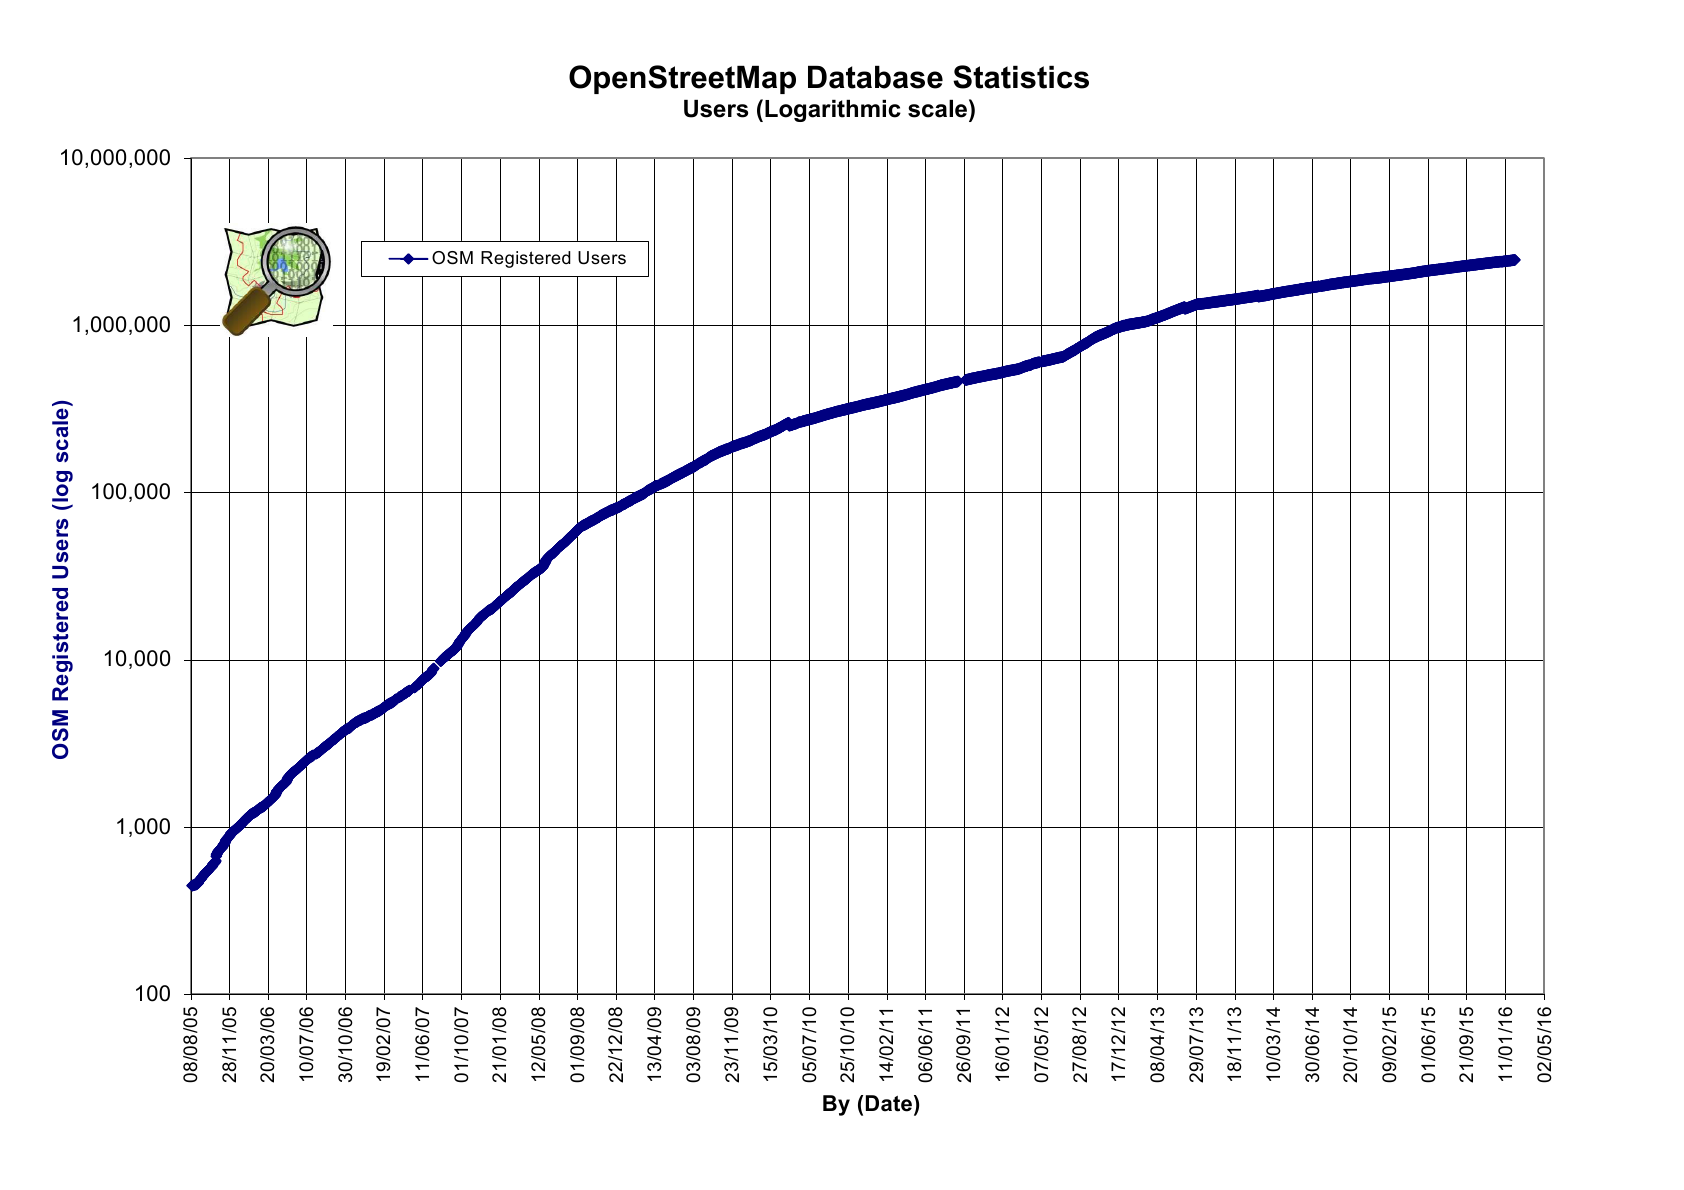
\includegraphics[width=.5\linewidth]{img/21a-Osmdbstats1_log.png}}\hfill
                    \subfloat[\label{obr21b}]
                    {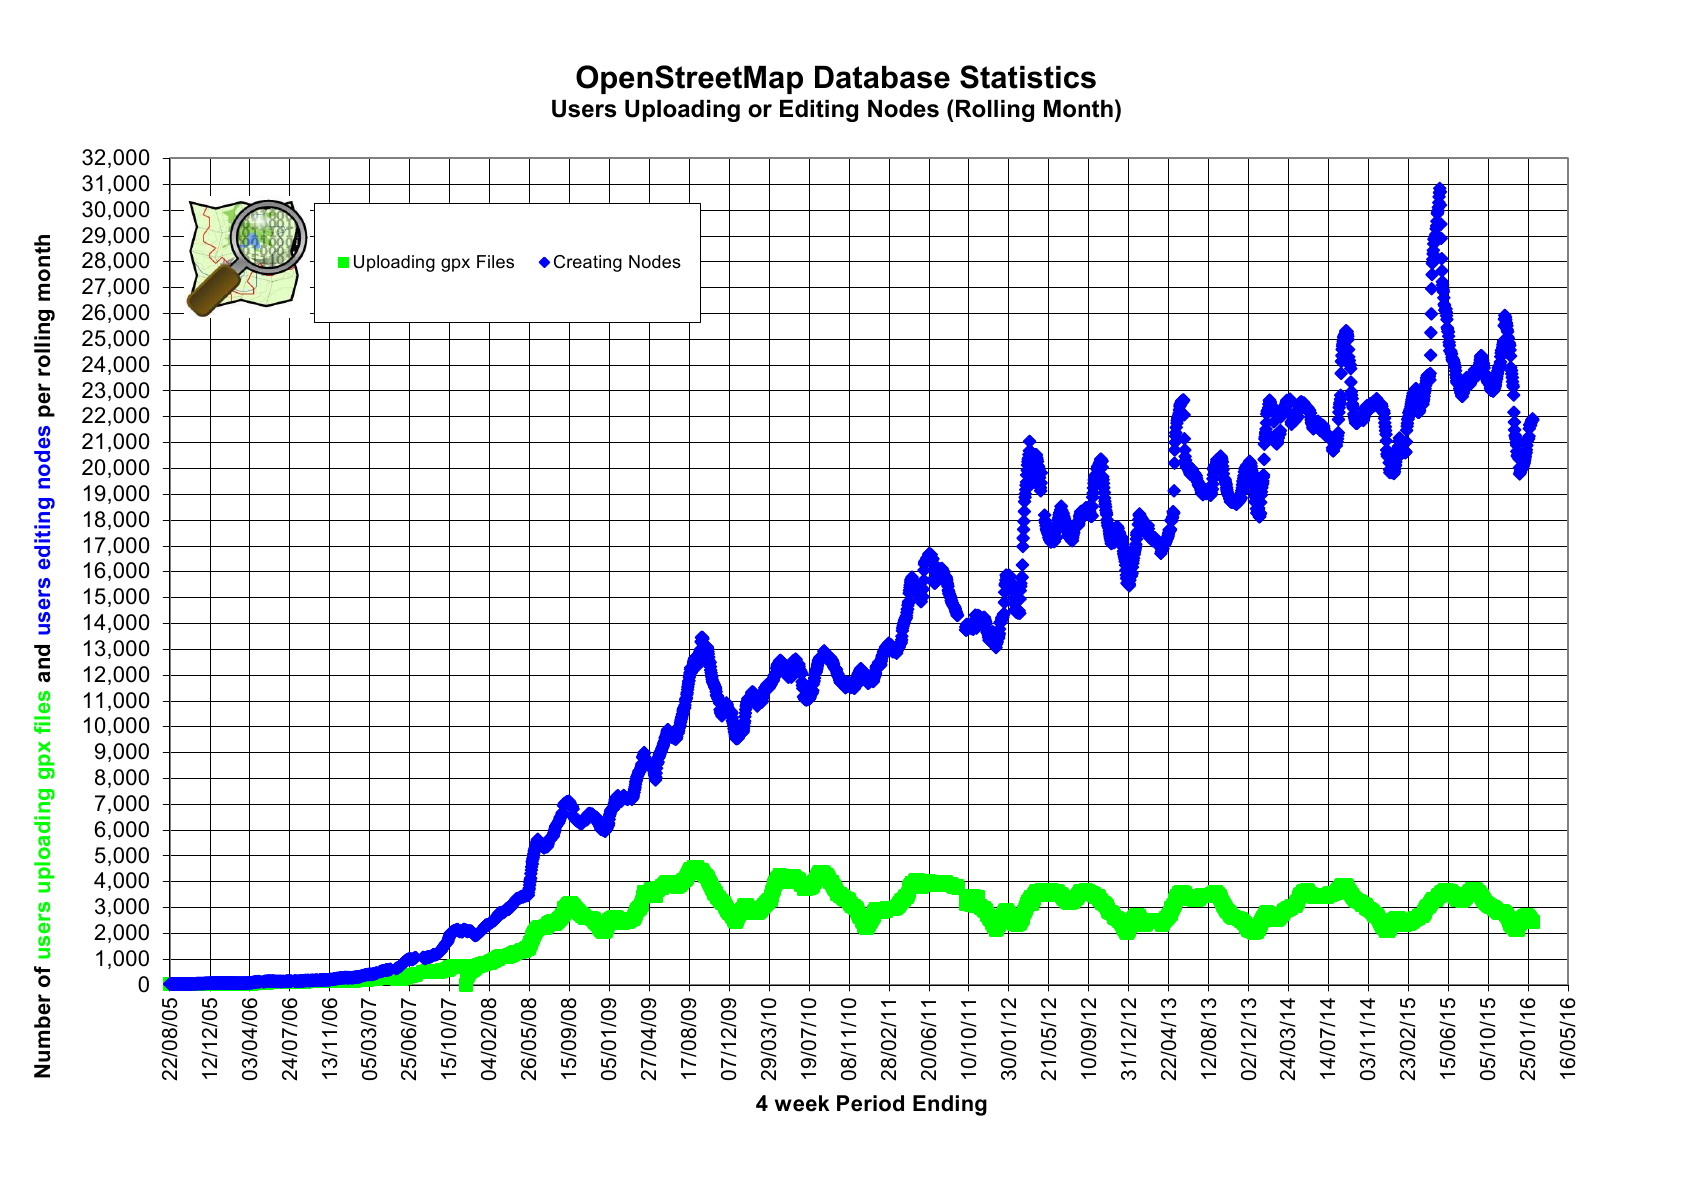
\includegraphics[width=.5\linewidth]{img/21b-Osmdbstats4A.png}}

                    \caption{Počet registrovaných uživatelů v~OSM (log. měřítko) (a); aktivní~uživatelé za měsíc v~modré barvě (b)\cite{zdroj39}}
                    \label{obr21}
                    \end{figure}
                    

Technicky se jedná o~vektorovou mapovou databázi, kterou může upravovat každý zaregistrovaný uživatel. Pokud se tedy někdo rozhodne zmapovat třeba všechna piána na ulicích, může si na to vytvořit vlastní značku a do databáze je přidat. Omezení je jediné, aby byl objekt fyzicky přítomný~v~reálném světě. To se samozřejmě týká i vnitřků budov.

Aby to vše dobře fungovalo, udržuje světová komunita OpenStreetMap společný značkovací klíč~(tzv. Map Features), který globálně určuje, jak se budou určité objekty značit. Díky tomu je možné vykreslit silniční síť celého světa, či najít cyklistickou trasu z~Madridu na Sibiř. Ke společné shodě dochází pomocí procesu tzv. proposals (návrhů).

Značkovací klíč -- též tagování -- je k~dispozici i v~českém překladu\footnote{\href{http://wiki.osm.org/Cs:Map\_Features}{wiki.osm.org/Cs:Map\_Features}}. Obsahuje hlavní kategorie všech objektů, další upřesnění jsou pak k~dispozici na stránkách jednotlivých značek. Ovšem to, že je například lavička ve značkovém klíči~neznamená, že by v~OpenStreetMap byly zaneseny všechny lavičky na světě. To vždy záleží na místní komunitě a zejména konkrétních přispěvatelích, co se kdo rozhodne mapovat. Česká komunita je jedna z~těch aktivnějších, a tak jsou v~ČR zmapovány všechny hlavní silnice, čísla popisná či třeba velké množství turistických značek a cyklotras.\cite{zdroj40}

Indoor mapování je pro OpenStreetMap přirozenou výzvou, a proto nepřekvapí, že přispěvatelé již tímto směrem vyvinuli nemalé úsilí. Do nynějška ovšem žádný návrh přijatý nebyl, proto se v~této práci pokusíme využít získaných poznatků, poučit se z~chyb a navrhnout řešení, které bude mít šanci na úspěch. Více v~kapitole 2.4.

Tak jako Steve Coast~měl v~roce 2004 vizi o~celosvětové mapě ulic, tak my nyní můžeme předestřít vizi celosvětové indoor mapy tvořené uživateli. Výhody jsou nasnadě, z~volných geodat a jednotného formátu pro celý svět může vzniknout množství velmi zajímavých aplikací. Příklady jsou k~vidění už dnes. Za všechny uveďme aplikaci Maps.me -- pro všechny mobilní platformy umožňuje offline zobrazení mapy včetně 3D budov, navigaci či editaci bodů zájmu samotnými uživateli.

Otevřená data vždy přilákají mnoho firem a tvůrců aplikací, a díky tomu vzniknou i nová a nečekaná využití. Může se jednat o~různé prohlížeče, aplikace veřejných institucí pro návštěvníky s~integrací mapy, prodejce nemovitostí, navigaci osob se sníženou schopností orientace, či zcela globální prohlížeč map včetně indoor režimu.

\section{Core architektura}\label{core-architektura}

Pojďme si nyní ukázat, na čem je OpenStreetMap postaveno -- vnitřní způsob ukládání dat, API a základní nástroje pro pokročilou práci.

Mapová data nejsou jako v~klasickém GISu objekty s~geometrií. Místo toho se využívá specifické schéma, které má tu výhodu, že zachovává topologii a je tak přímo vhodné jako routovací graf. Základní prvky jsou tyto:

\begin{itemize}

\item
  uzel~(node) -- bod, který jako jediný nese souřadnice,
\item
  cesta~(way) -- posloupnost referencí na uzly; nejde o~cestu v~běžné řeči, ale v~terminologii OSM, význam jí dodávají až aplikované tagy, ~
\item
  relace (relation) -- reference více uzlů, cest a relací.
\end{itemize}

Samotný význam je pak možné ke každému primitivnímu prvku přidávat v~podobě libovolných značek -- tagů. Krom toho ještě cesta může znamenat i plochu -- to v~případě, kdy je uzavřená a nese určité tagy (třeba \texttt{area=yes}). Tímto je tedy výčet úplný:

\begin{itemize}

\item
  značka (tag) -- klíč a hodnota (např. \texttt{highway=residential}),
\item
  plocha~(area) -- uzavřená cesta, která nese určité tagy,
\item
  metadata~-- doplňkové informace pro správu dat (autor, id, verze, changeset).
\end{itemize}

Editace se provádí pomocí API tak, že uživatel pošle upravené prvky v~rámci jednoho změnového požadavku, tzv. changesetu. V~databázi se pak vytvoří nové prvky a upraví ty stávající zvýšením verze. Smazání se provede nastavením příznaku visible, technicky tedy jde pouze o~úpravu. V~případě vandalské editace je tak možné celý changeset odvolat (revert) a vrátit data do původní podoby.

\subsection{Data a OSM XML}\label{data-a-osm-xml}

Data se ve většině případů reprezentují ve formátu OSM XML. Uveďme si jednoduchý příklad (obrázek \ref{obr22}).~Obsahuje tři uzly, z~nichž rozcestník stojí zcela samostatně a dva uzly jsou referencovány v~rámci cesty. Jeden z~těchto uzlů v~cestě nese zároveň další vlastnost -- pomníček.

Relace sdružuje všechny zmíněné prvky a vytváří turistickou trasu \uv{Odbočka k~pomníčku}, kde definuje její barvu, referenční číslo i symbol, který má být vykreslen.

Informace o~topologii -- napojení cest -- je tak dána referencováním ID stejného uzlu. Již je ponecháno na konzumentovi dat, aby získal pouze relevantní prvky (typicky cesty s~tagem \texttt{highway=*}) a následně si z~dotažených uzlů vynesl geometrii cest a spočítal ohodnocení hran.

Relace v~principu přenáší své tagy na jednotlivé členy. Doporučuje se tedy používat pouze tam, kde je skutečně potřeba. Kvůli horší možnosti editace je například nevhodná pro sdružování více cest tvořící jednu ulici. Naopak rozsáhlejší sdružení objektů, typicky turistické trasy, jsou v~relacích vítané, neboť se lépe udržují a též je umožněno využít jedné fyzické cesty pro vedení více tras. Členy navíc mohou mít v~dané relaci uvedenou roli.

 \begin{figure}
	  \centering
      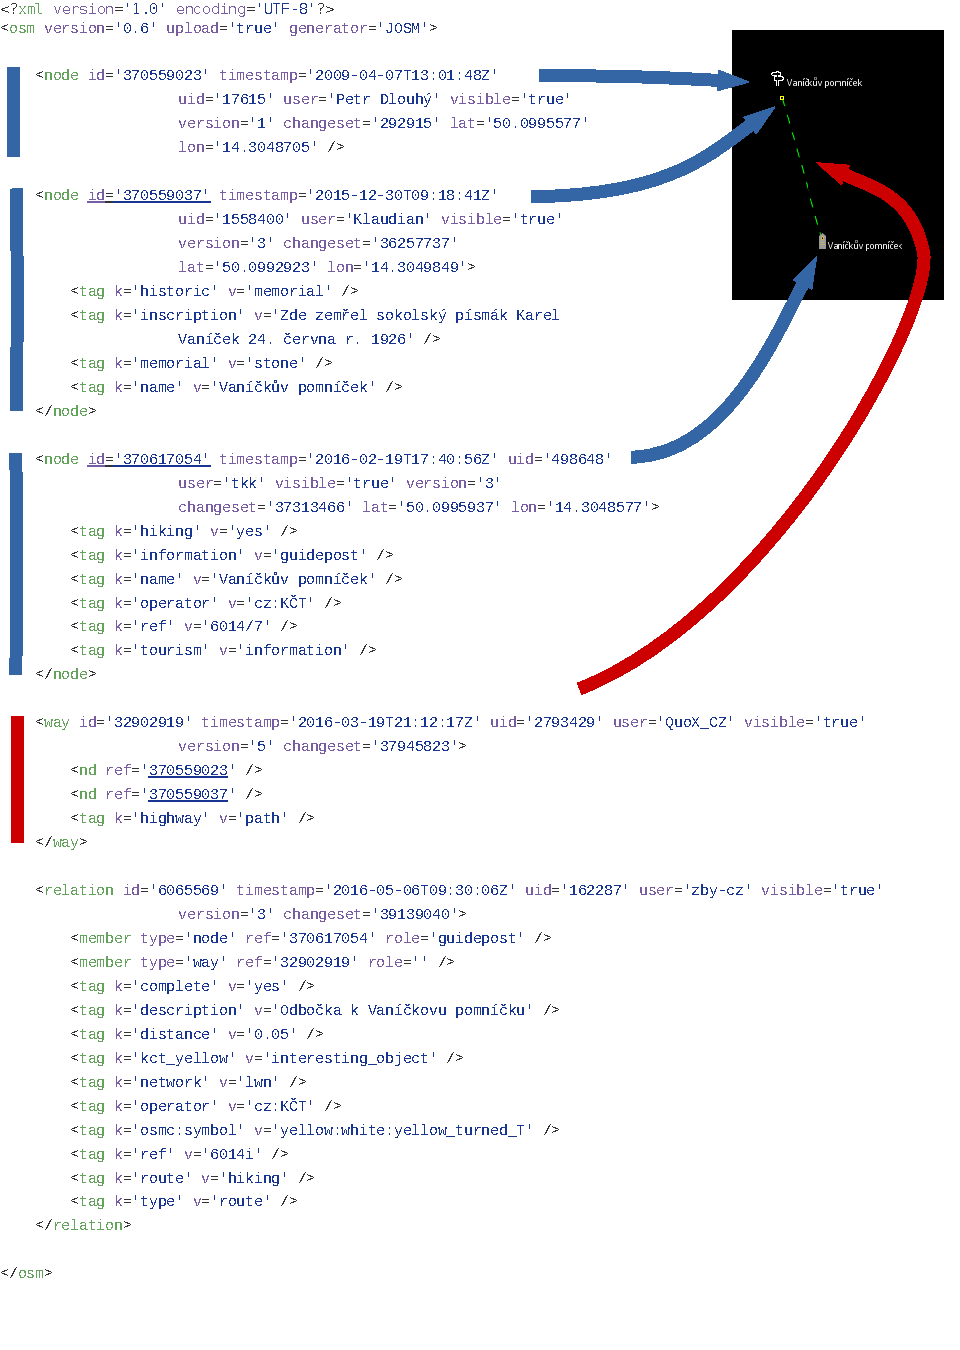
\includegraphics[width=\textwidth]{img/22-osm-xml-ex.pdf}
      \caption{Ukázka formátu OSM XML a reprezentace v~editoru JOSM\cite{zdroj41}}
      \label{obr22}
  \end{figure}

Nejčastěji používané typy jsou tyto, určují se tagem \texttt{type=*:}

\begin{itemize}

\item
  Route~-- vedení turistických, cyklistických tras, či trasy MHD, trajektů apod. (viz příklad).
\item
  Multipolygon~-- jednak umožňuje ploše vymezit, kde se nenachází (tj. ohraničit díru), jednak pro rozsáhlé plochy (lesní porost) umožňuje sdružit více okrajových cest. Ty jsou děleny z~důvodu snazší práce v~editorech.
\item
  Boundary~-- sdružuje okrajové cesty územních hranic a též relace podřízených oblastí. Například relace České republiky bude obsahovat všechny hraniční cesty~(ve smyslu cesty v~OSM) a relace všech krajů.
\item
  Restriction~-- zaznamenává zákazy odbočení, které implicitně neplynou z~jednosměrek.
\end{itemize}

Díky velké rozmanitosti získávání dat je možné narazit na různé zápisy téhož. Zejména bod zájmu (např. pomníček) může být ve vztahu k~přístupové cestě~reprezentován:

\begin{itemize}

\item
  uzlem~(na konci pěšiny i mimo ní) -- přibližná poloha objektu,
\item
  plochou~(napojenou i nenapojenou na cestu) -- značící přesnější obrys fyzického objektu,
\item
  relací~multipolygon~(opět napojenou nebo jen \uv{poblíž}) -- značící složitější plochu .
\end{itemize}

\subsection{API a další služby}\label{api-a-dalux161uxed-sluux17eby}

Samotná databáze OpenStreetMap je hlavní centralizovaný zdroj, do kterého se ukládají všechny editace. Aby bylo možné mapová data dále využívat, existuje několik služeb, která je poskytují navenek.

\begin{itemize}

\item
  API~-- obsahuje nejčerstvější data a je určeno pouze pro účely editace. Umí vrátit všechna data v~požadovaném výřezu\footnote{Volání \href{http://api.openstreetmap.org/api/0.6/map?bbox=14.304,50.099,14.306,50.1}{api.openstreetmap.org/api/0.6/map?bbox=14.304,50.099,14.306,50.1}}~a uložit upravené objekty zpět. Krom toho nabízí zdroje~pro práci s~historií, changesety a uživatelskými profily. Komunikuje pomocí OSM XML. Pro autentizaci používá mimo jiné OAuth 1.0.~Více na \href{http://wiki.osm.org/API}{wiki.osm.org/API}
\item
  Planet dump~-- jednou týdně proběhne export celé databáze do formátu OSM XML s~kompresí bzip2 (osm.bz2) a Google protobuf formátu (osm.pbf). K~dispozici jsou dvě verze: mapa bez historie (49 GiB, resp. 32 GiB) a s~kompletní historií (75 GiB, resp. 51 GiB). Též se nabízí různé změnové soubory (osc) v~týdenním, denním i minutovém rozsahu. Více na \href{http://planet.openstreetmap.org}{planet.openstreetmap.org}
\item
  Overpass API~-- rozhraní optimalizované na čtení data a vykonávání i poměrně složitých dotazů. Funguje v~zásadě jako databáze přes protokol HTTP. Hodí se pro jednorázové exporty zájmových skupin prvků i pro pravidelné využití pro backend~různých webových aplikací. Umožňuje dva dotazovací jazyky a výstup v~OSM XML či JSON, bohužel chybí přímá podpora pro GeoJSON.\\
  Více informací na \href{http://wiki.osm.org/Overpass\_API}{wiki.osm.org/Overpass\_API}, grafické rozhraní \\ na \href{http://overpass-turbo.eu}{overpass-turbo.eu}
\item
  XAPI~-- kopie API pouze pro čtení s~povolenou větší zátěží. Dnes nahrazena Overpassem.
\item
  Exporty~-- několik dalších serverů nabízí předzpracovaná data z~exportu Planet dump. Metro extracts nabízí vyříznuté oblasti velkých měst\cite{zdroj42}, Geofabrik.de nabízí výřezy pro jednotlivé kontinenty a státy\cite{zdroj43}.
\end{itemize}

\section{Editory}\label{editory}

Tak jako existuje mnoho služeb, vzniklo komunitním vývojem i přes desítku editorů pro úpravu OpenStreetMap. Podívejme se pouze na ty současné, na jejich charakteristiky i případné schopnosti tvořit indoor mapy.

\subsection{JOSM}\label{josm}

JOSM je pokročilý editor určený pro pokročilé uživatele. Je postaven na platformě Java, takže jej~lze spustit na všech operačních systémech. Vývoj začal v~roce 2006 a od začátku se vyznačoval velkou rozšiřitelností. V~současnosti čítá přes 200 pluginů, 100 rozšířených předvoleb tagování (presets) a mnoho vykreslovacích stylů. Velikou nevýhodou je nepřehlednost uživatelského rozhraní, proto není vhodný pro začátečníky.

Využívá společný editor-layer-index\cite{zdroj44}~pro definici mapových a ortofoto vrstev, ze kterých je možné odvozovat data. Tam se kromě serverů s~globálním pokrytím nachází i mnoho regionálních, které jsou nabídnuty podle aktuálního místa editace.

Vyznačuje se možností práce offline, a tedy i načítání větších datasetů či mnoha záznamů GPS trasy (GPX soubory). Kromě načtení klasického výřezu z~API umí stahovat i jednotlivé prvky či kompletní relace. Obsahuje také přímé napojení na Overpass API. Pomocí pluginů pak například načítá fotky z~otevřeného street view Mapillary, či vykresluje výšky objektů dle metodiky Simple 3D.

Pro pohodlnější editaci nabízí možnost vlastního filtrování dat dle zadaného dotazu. Tato vlastnost je základní funkcionalitou~nutnou~pro indoor mapování. Tagovací předvolby a vykreslovací styly pro některé indoor metodiky jsou~již~také k~dispozici, případně je možné je snadno vytvořit.

 \begin{figure}
	  \centering
      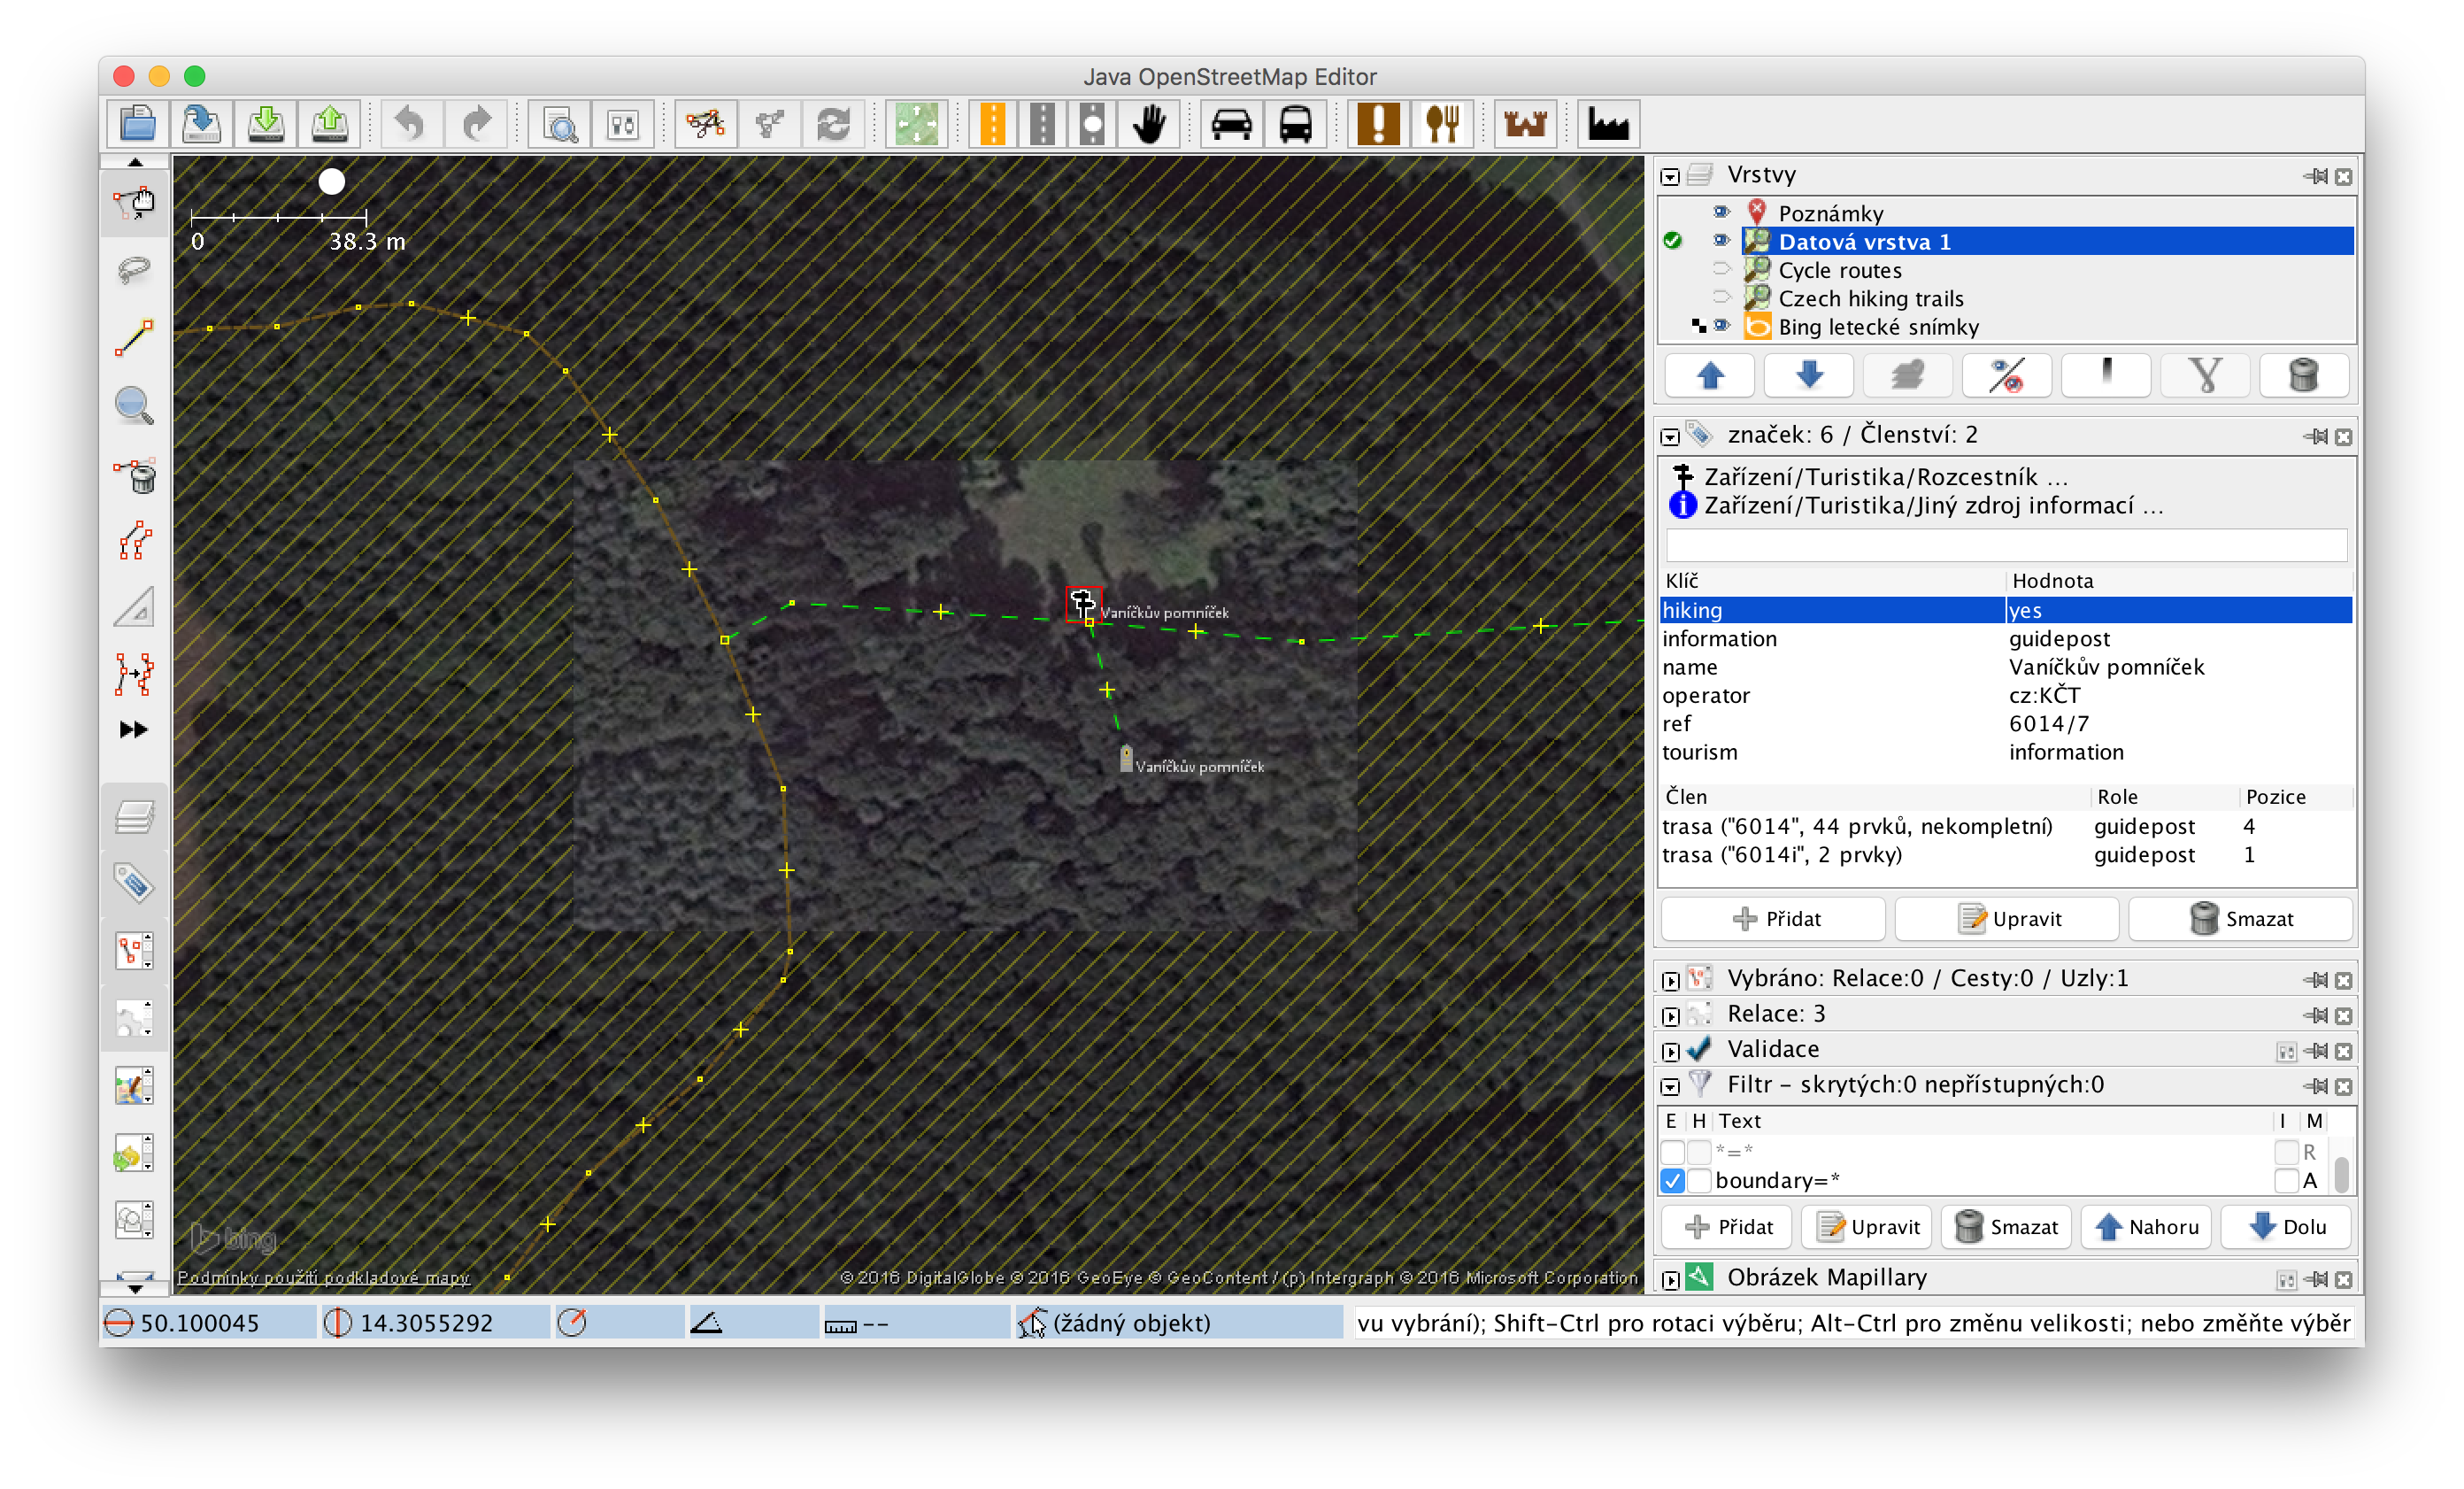
\includegraphics[width=\textwidth]{img/23-editor-josm.png}
      \caption{Editor JOSM}
      \label{obr23}
  \end{figure}

\subsection{Potlatch2}\label{potlatch2}

Online webový editor na platformě Flash, který byl v~aktivním vývoji 2009--2013. Na vlastním vykreslovacím jádře umí svižně zobrazovat i editovat data a disponuje i několika pokročilými funkcemi. Nyní již je na ústupu, neboť neumožňuje tak snadnou rozšiřitelnost a protože technologie Flash přestává být podporována ve prospěch HTML5.

Pro indoor mapování~nemá podporu -- vykresluje prvky všech pater současně.

 \begin{figure}
	  \centering
      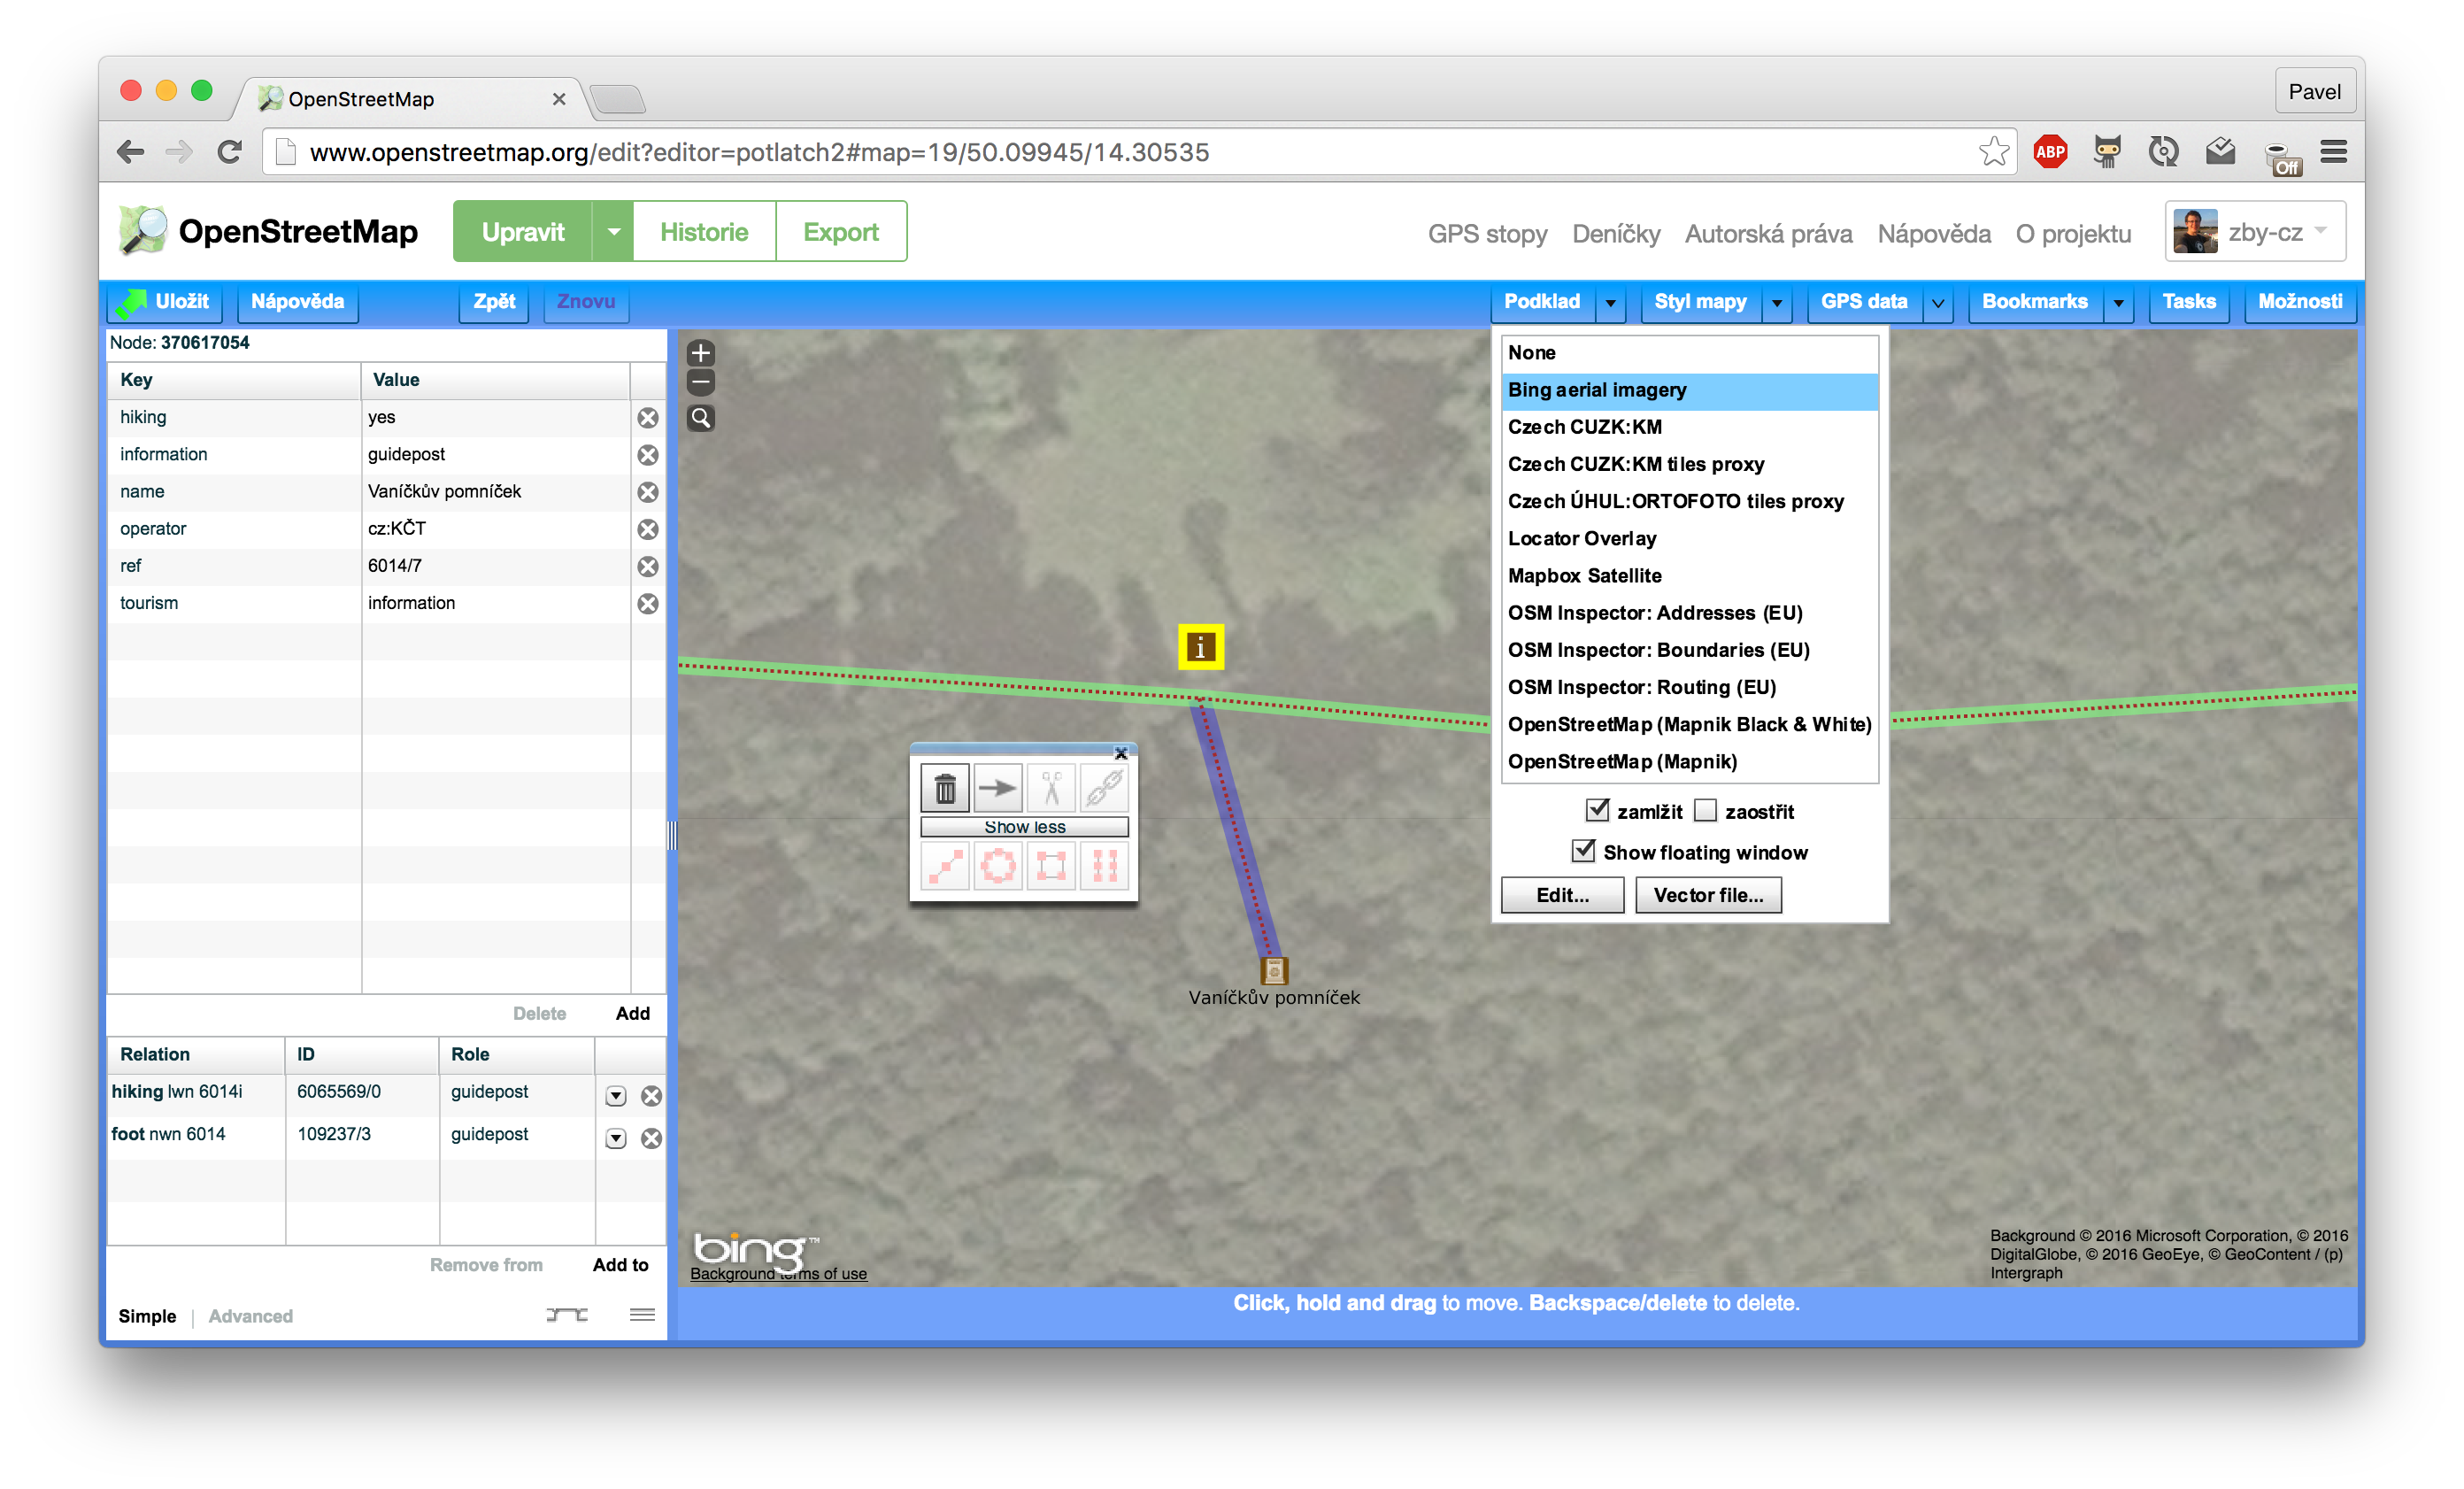
\includegraphics[width=\textwidth]{img/24-editor-potlatch2.png}
      \caption{Editor Potlatch2 s~rozbalenou nabídkou podkladů}
      \label{obr24}
  \end{figure}

\subsection{Editor iD}\label{editor-id}

Nový webový editor iD je postaven na technologiích HTML5. Úsilí začalo v~roce 2012, kdy byl podpořen grantem Knights foundation\cite{zdroj45}~a vývoj koordinován společností MapBox. Hlavní vývoj probíhal v~roce 2013, kdy byl i nasazen jako výchozí editor na stránce openstreetmap.org.

iD je narozdíl od ostatních editorů navržen zejména s~ohledem na jednoduchost použití. Po spuštění uživateli nabídne interaktivní komentovanou prohlídku základů editace. Zřetelně odlišuje kreslicí a prohlížecí módy a nabízí bohaté formuláře s~přednastaveným tagování (presets). V~režimu přímého zadávání tagů pak nabízí již existující tagy dle databáze taginfo.

 \begin{figure}
	  \centering
      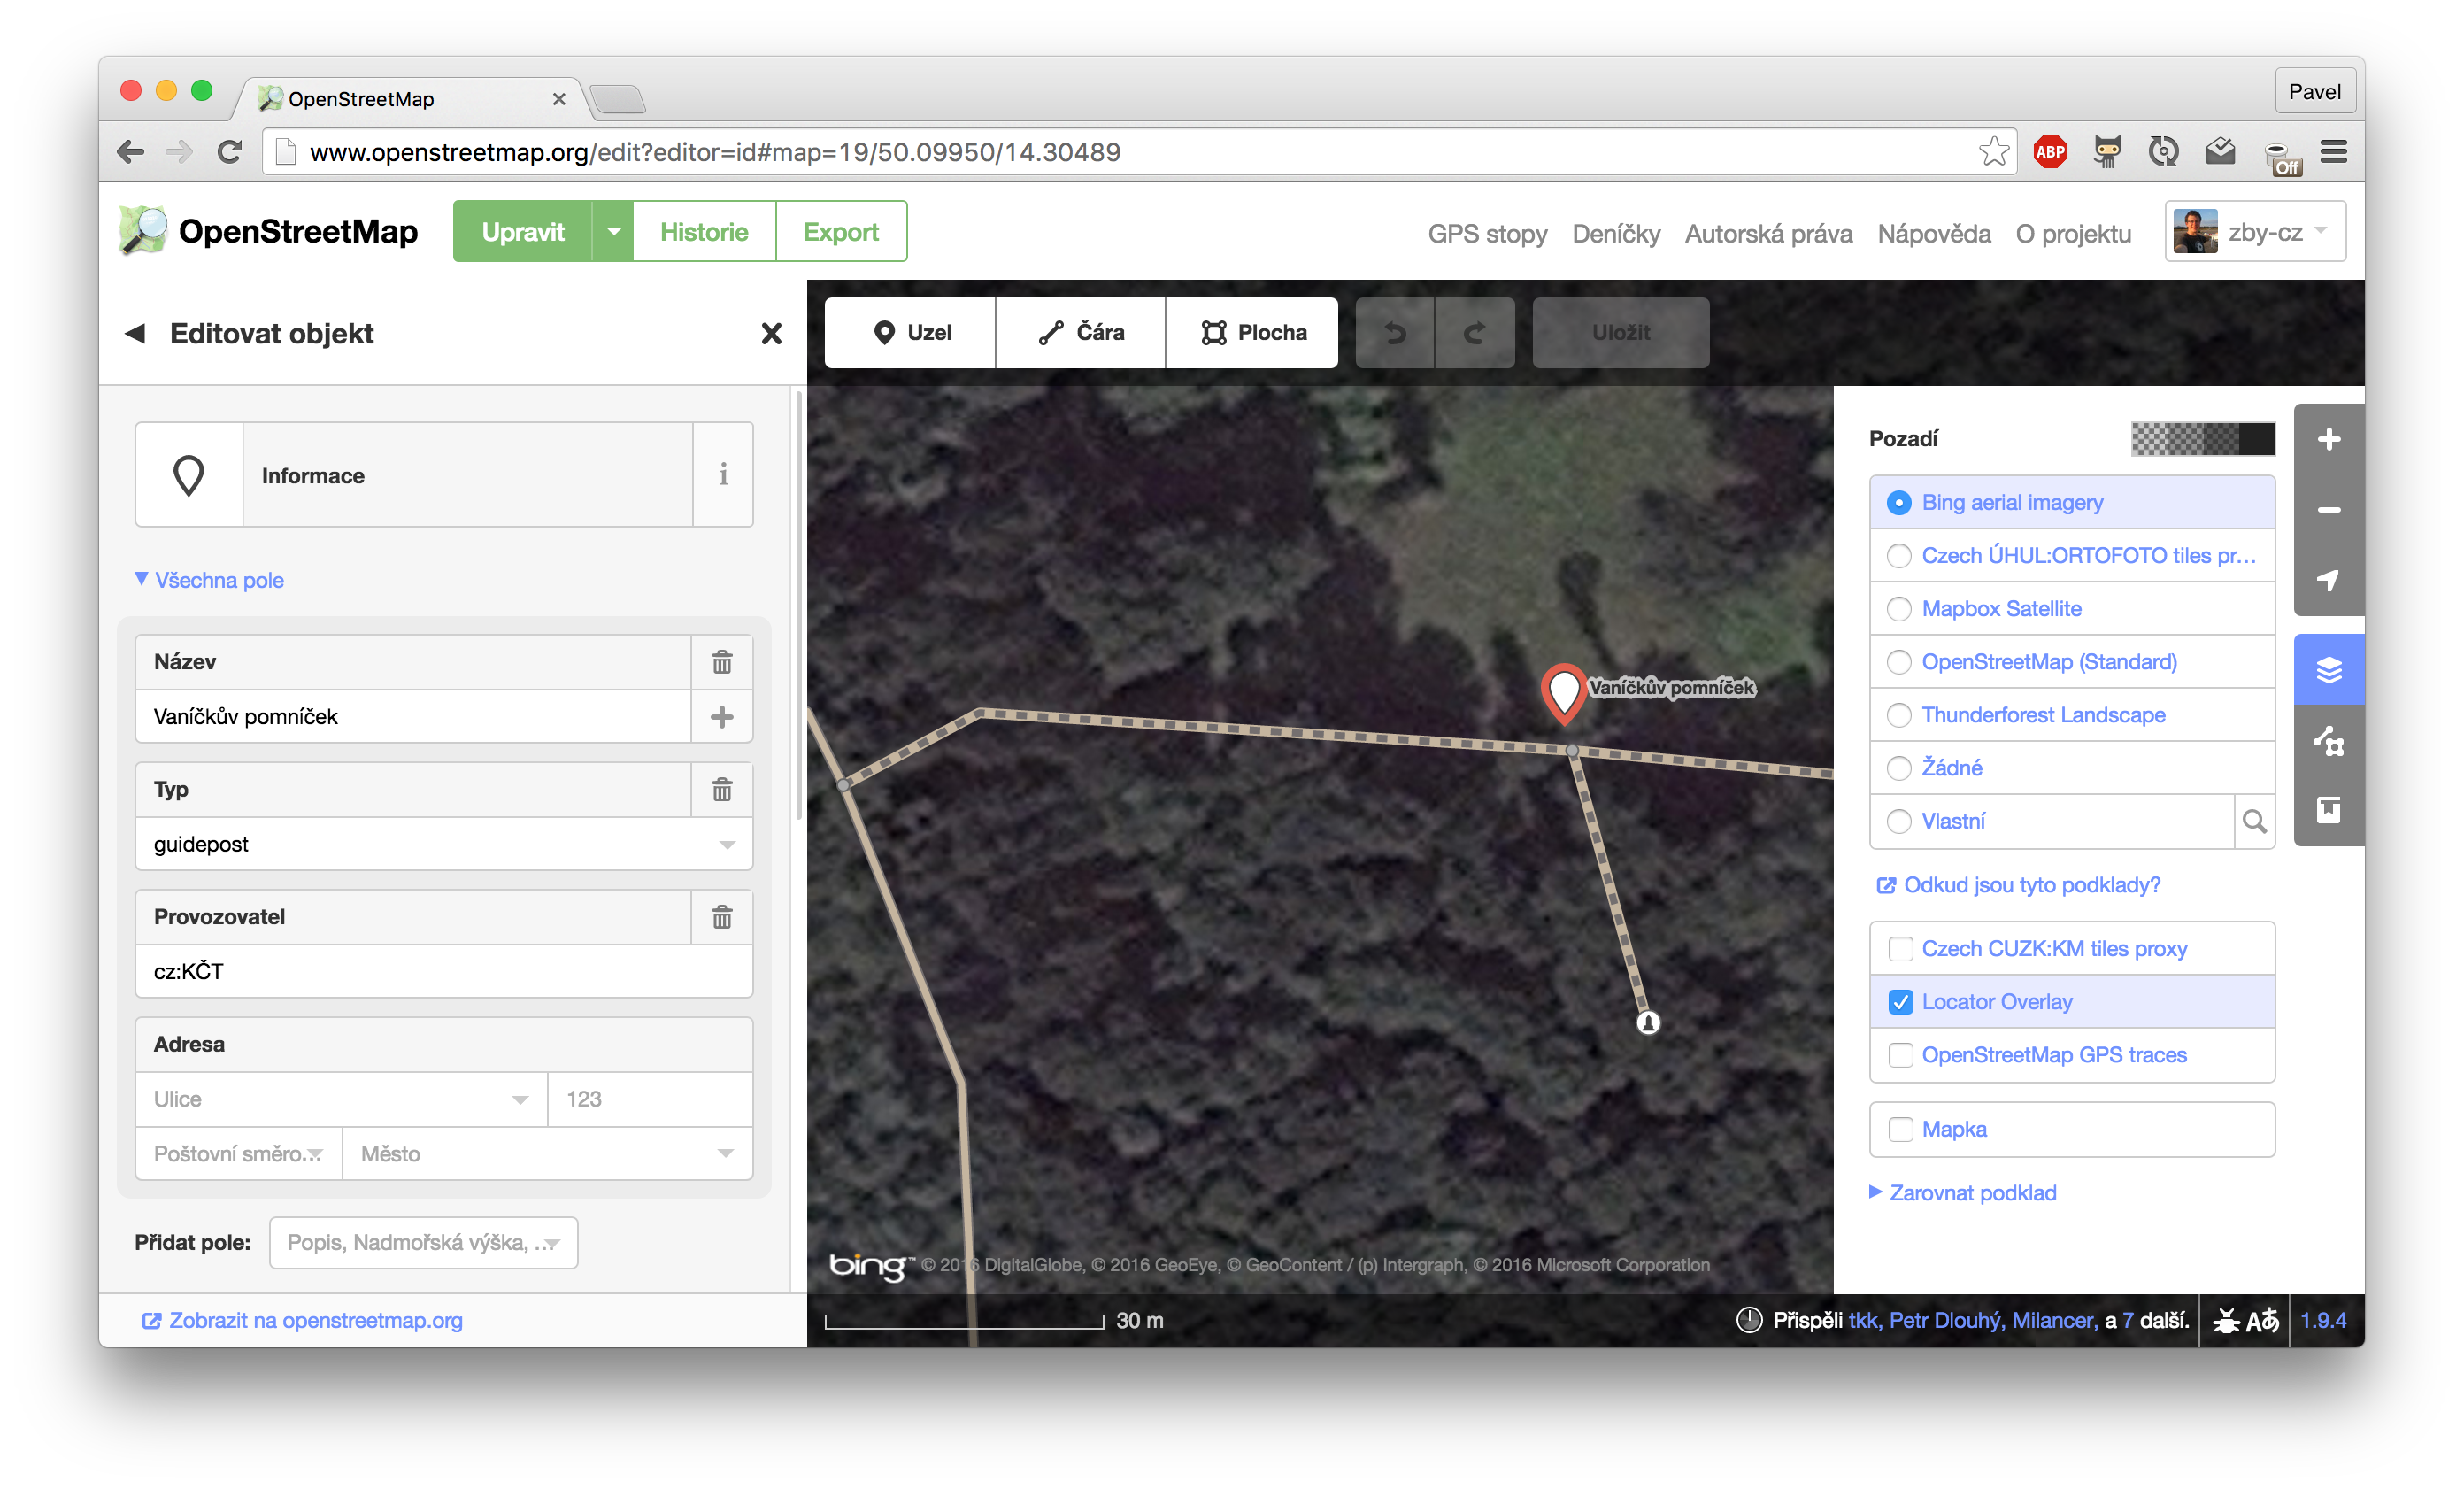
\includegraphics[width=\textwidth]{img/25-editor-id.png}
      \caption{Editor iD s~vybraným uzlem rozcesníku}
      \label{obr25}
  \end{figure}

Z~technologií HTML5 využívá pokročilou vizualizační knihovnu d3.js. Vykreslení přenechává na inline SVG, které lze výhodně stylovat pomocí klasického CSS3. Díky tomu lze editoru snadno upravovat chování za běhu a vyvíjet nové vlastnosti (tzv. hackable editor).

Pro indoor mapování nemá podporu -- vykresluje všechny prvky všech pater současně.

\section{Indoor v~OSM}\label{indoor-v-osm}

Jak již bylo naznačeno v~úvodu této kapitoly, indoor mapování v~OpenStreetMap už prošlo určitým vývojem. Vzniklo několik návrhů, které byly~vyzkoušeny v~praxi, proběhlo několik pokusů o~tvorbu editoru a neposledně byly~zmapovány~stovky budov po celém světě (ačkoliv, s~trochou nadsázky, každá mírně jinou metodikou).

Tato práce se nesnaží o~nalezení zcela nového způsobu tagování, ale staví na tom,~co je dobře navrženo,~a přidává i ubírá tak, aby byl výsledek pro komunitu~přijatelný.

\subsection{Výzvy pro indoor mapování}\label{vuxfdzvy-pro-indoor-mapovuxe1nuxed}

Architektura OpenStreetMap je navržená velmi flexibilně a nemá potíž se začleněním indoor dat. Existují však některé technické i netechnické výzvy, které je dobré promyslet. Na OSM wiki\cite{zdroj46}~je sepsal uživatel Dave Sutter.

\begin{enumerate}

\item
  Data jsou svým charakterem trochu jiná -- nekreslí se v~jedné vrstvě, ale každé patro má svou vrstvu. Naopak klasické 2D mapy jsou nyní ploché, zobrazují vše v~jedné vrstvě. V~případě bodů zájmu to může být žádoucí, pokud jich není mnoho na stejných souřadnicích, ovšem v~případě překrytí mírně odlišných komunikací~vznikne nesrozumitelný výstup. Způsobeno je to také tím, že pro některé indoor i venkovní prvky (například chodník) se používá stejné tagování, takže renderer je vykreslí v~obou případech.\\
  Editory vždy vykreslují všechna data, takže problém je ještě markantnější.
\item
  Business listingy se, obzvlášť v~nákupních centrech, mohou často měnit, geometrie však zůstává. Tento bod adresuje obecnější problém, jak se má OSM postavit ke katalogizaci firem. V~ideálním případě by existoval volný katalog firem se všemi údaji, otvírací dobou apod. a v~OSM by byla uložena~jen geometrie + prolinkování do katalogu. Ovšem naděje na vznik podobného katalogu jsou mizivé.
\item
  Právní důsledky -- mapování veřejného prostoru je v~pořádku, například nákupní centra ale bývají vlastněna soukromými subjekty a k~získávání dat je vhodný souhlas.
\item
  Dočasné mapy -- například pro různá výstaviště je typické, že každoročně staví stejné schéma pro jeden konkrétní veletrh. V~tuto chvíli není vhodný způsob jak tuto informaci do OSM uložit. Pokud se geometrie v~databázi zanechají s~jinými tagy a přes ně se budou kreslit data pro \uv{aktuální veletrh}, bude v~databázi nepřehledná změť čar. Toto je opět výzva pro editory i mapové výstupy.
\end{enumerate}

\subsection{Dřívější pokusy}\label{dux159uxedvux11bjux161uxed-pokusy}

Abychom se mohli poučit z~předchozích návrhů, pojďme si je shrnout. Díky tomu, že v~OSM je možné používat i neschválené tagování, mohli autoři vytvořit mnoho příkladů použití.

\subsubsection{Level relation -- 5/2009}\label{level-relation-52009}

Jedná se o~krátký návrh na vytvoření relace sdružující všechny objekty na jednom patře s~tím, že vícepatrové budou mít příslušnost k~více relacím. Tento koncept se opakuje i v~následujících návrzích.~Uvádí také základ tagu \texttt{level=*}~s~významem \texttt{level=0}~jako přízemí a možností tagování mezipater desetinným číslem.

K~dispozici na: \href{http://wiki.osm.org/Relations/Proposed/Level}{wiki.osm.org/Relations/Proposed/Level}~

\subsubsection{Indoor by saerdnaer -- 3/2011}\label{indoor-by-saerdnaer-32011}

Komplexnější návrh z~Technické univerzity v~Mnichově opět využívá relace pro jednotlivá patra, ale zavádí i některé další užitečné koncepty.


                      \begin{figure}
                    
                    \subfloat[\label{obr26a}]
                    {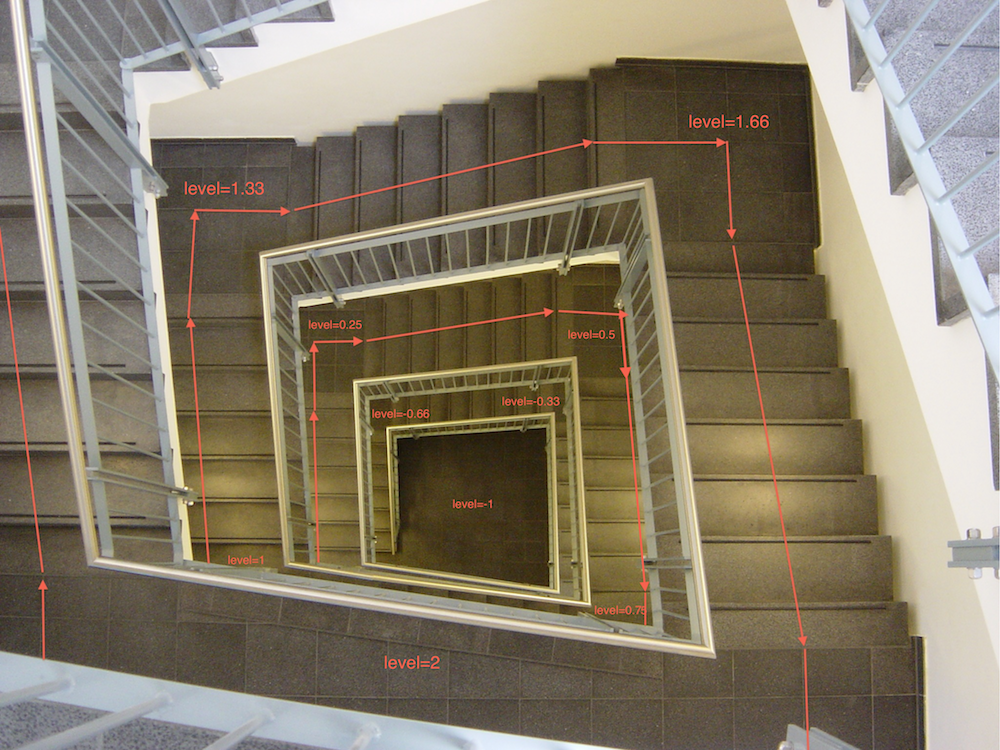
\includegraphics[width=.5\linewidth]{img/26a-Indoor_steps1.png}}\hfill
                    \subfloat[\label{obr26b}]
                    {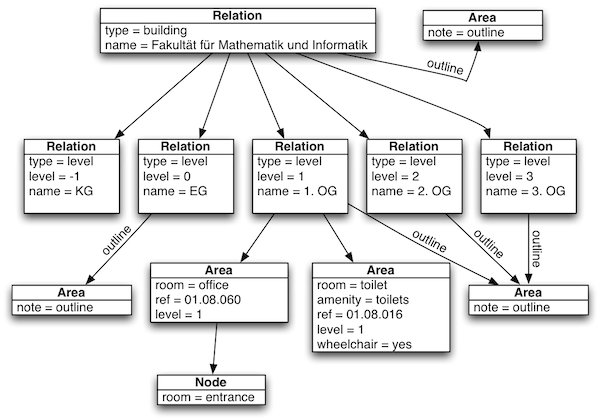
\includegraphics[width=.5\linewidth]{img/26b-Indoor_relations.png}}

                    \caption{Desetinný level u~schodů (a); přehled relací pater (b)\cite{zdroj47}}
                    \label{obr26}
                    \end{figure}
                    

Jednotlivé místnosti označuje plochami s~tagem \texttt{room=*}, kde se využívá rozlišení typů dle SIG3D (součást CityGML -- viz kapitola 1.1.8). Dále využívá již dobře ustanovené tagy: \texttt{ref=*}~pro číslo místnosti, \texttt{entrance=*}~pro vchody a \texttt{access=*}~pro omezení vstupu.

Chodby nemodeluje jako plochy, ale liniově vedené cesty s~novým tagem \texttt{highway=corridor}. Tak je to v~OSM zvykem a zároveň je tím tvořen routovací graf. Pro venkovní vedení přidává \texttt{outdoor=yes}.

Pro \texttt{level=*}~ukazuje, jak by mohlo být tagováno schodiště, zejména v~případě, že na různých odpočívadlech vedou dveře jinam. Kromě uvádění levelu~v~relacích také uvádí alespoň jeden \texttt{level=*}~u~samotného prvku.

K~dipozici na: \href{http://wiki.osm.org/Proposed\_features/indoor}{wiki.osm.org/Proposed\_features/indoor}~pouze v~německém jazyce

\textbf{Naše hodnocení:}~Dobře zpracovaný návrh, který už je nahrazen jinými. Využíval principů OSM (uzly, cesty) a existujících tagů (access, \ldots{}), měl přesah do CityGML a využíval pokročilejších vlastností tagu level, který i přenášel na jednotlivé prvky.

\subsubsection{Level\_map -- 9/2011}\label{levelux5fmap-92011}

Zcela vyčerpávající návrh~čítající 8 stran textu popisuje poměrně složitý systém využití relací a rolí. Využívá též možnosti replikace objektů, které se nachází ve více patrech na stejném místě (např. chodba, toalety). Objekt je pak v~OSM databázi jen jednou, ale je přiřazen do více pater.

Jeho hlavním stavebním kamenem je relace \texttt{type=level}\_map. Přiřazuje uspořádaný seznam ID pater v~objektu do tagu \texttt{levels=*}, např. \\ \texttt{levels=B;G;1-3} (pro Basement, Ground floor a patra). Zde nabízí i možnost rozšířeného pojmenování pater pomocí \texttt{levels=B=Basement;\ldots{}} či specifikaci výšky v~metrech a dalších jazykových překladů.

Všechny objekty v~budově jsou~pak členy této relace a jejich role udává patro. Návrh~nabízí i speciální role pro spojení více pater (schodiště) či dokonce možnost definovat nové pojmenované~role s~pokročilými možnostmi. Do rolí též navrhuje psát možné odlišnosti v~tagování objektu v~různých patrech, např. \texttt{role:Toilets=B;3[female=yes;male=no];4[female=no;male=yes]}.

K~dipozici na: \href{http://wiki.osm.org/Relations/Proposed/Level\_Map}{wiki.osm.org/Relations/Proposed/Level\_Map}

\textbf{Naše hodnocení:} návrh není vhodný, kvůli své složitosti. Vytváří zbytečně několik nových syntaxí uvnitř (textového) tagu, zavádí identifikátory pro složitější popis rolí a nevyužívá tedy dobře existující architekturu prvků a tagů. Implementace editoru i prohlížeče by byla velmi náročná.

\subsubsection{IndoorOSM -- 11/2011}\label{indoorosm-112011}

Jeden z~úspěšnějších návrhů~z~Universität Heidelberg\cite{zdroj48}~dal za vznik i editoru a prohlížeči. V~současné době je zamítnutý ve prospěch Simple Indoor Tagging.

Definuje jednu hlavní relaci pro budovu \texttt{type=building}, která sdružuje podrelace pater a zároveň obsahuje další informace o~budově, včetně některých navržených vlastností pro 3D vzhled. Samotná relace patra \texttt{type=level}~pak udává číslo i jméno patra a sdružuje jednotlivé objekty.

 \begin{figure}
	  \centering
      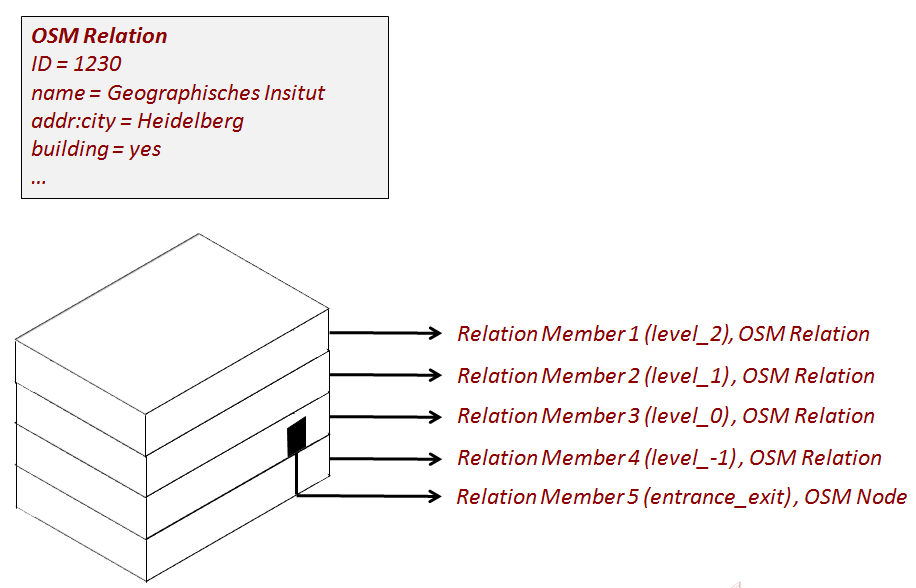
\includegraphics[width=\textwidth]{img/27-IndoorOSM-General.png}
      \caption{Relace budovy a její podrelace\cite{zdroj49}}
      \label{obr27}
  \end{figure}

Všechny indoor objekty (pokoje, chodby, atd.) navrhuje tagovat jako \\ \texttt{buildingpart=*}, např. \texttt{buildingpart=room}~apod. a též je umístit do relace patra v~roli buildingpart. Dveře a okna jsou zvoleny jako uzly s~možností vyplnit šířku, výšku, omezení vstupu apod. Prvky mají definováno patro pouze přes příslušnost k~relaci, tag \texttt{level=*}~na nich tedy není vyžadován.

Propojení mezi patry je řešeno netradičním způsobem. Každý prvek, který se propojuje do jiného patra, má na sobě tag s~ID uzlu \uv{kam je možné jít}, např. \texttt{connector:ids=67890}. Tento \uv{connector} je tedy jednosměrná informace pro routing. Pokud by šlo o~schodiště, tedy obousměrný segment, bylo by nutné vždy vzájemně referencovat uzly v~patrech nad sebou.

Díky větší aktivitě týmu z~univerzity i dalších zapojených lidí již bylo otagováno velké množství budov nejen v~Německu (dle taginfo existuje téměř 6~000 relací \texttt{type=building}\cite{zdroj50}) a vznikla řada nástrojů. Podívejme se na některé z~nich:

\begin{itemize}

\item
  javascriptový prohlížeč postavený na Overpass API\footnote{\href{http://clement-lagrange.github.io/osmtools-indoor/}{clement-lagrange.github.io/osmtools-indoor/}},
\item
  Indoor 3D -- prohlížeč indoor dat na systému OSMBuildings\footnote{\href{http://osmbuildings.org/indoor}{osmbuildings.org/indoor}},
\item
  univerzitní 2D i 3D prohlížeč\footnote{\href{http://indoorosm.uni-hd.de/}{indoorosm.uni-hd.de/}~a \href{http://indoorosm.uni-hd.de/3d/}{indoorosm.uni-hd.de/3d/}},
\item
  simulátor evakuace budovy v~prostředí MATSim,
\item
  Návod na editaci v~editoru JOSM na stránce návrhu.
\end{itemize}

K~dipozici na: \href{http://wiki.osm.org/IndoorOSM}{wiki.osm.org/IndoorOSM}

\textbf{Naše hodnocení:}~Tento návrh~komplexně řeší problematiku indoor mapování, uvažuje nad možností vykreslování ve 3D i navigací. Zadávání pomocí relací není snadné, ale je možné, jak se i prokázalo praxí. Hlavní nevýhodou je referencování ID uzlů, to autoři později sami označili za nevhodné, neboť toto ID se může měnit. Jistá nevýhoda může~též~plynout ze zaměnitelnosti tagu buildingpart~s~building:part, který je používaný pro metodiku Simple 3D buildings.\cite{zdroj51}

\subsubsection{Compound facility -- 11/2013}\label{compound-facility-112013}

Tento návrh z~Budapest University of Technology and Economics vznikl pro potřebu navigace cestujících v~rámci rozsáhlých stanic. Univerzitní tým připravoval multimodální plánovač tras a tento návrh~měl nastavit metodiku, jak tagovat indoor mapy s~ohledem na složitější modely pater a hledání tras v~napojených plochách.

Navrhuje podobný systém relací jako IndoorOSM. Hlavní relace \\(\texttt{type=compound}\_facility) sdružuje všechny vchody a podrelace jednotlivých pater (\texttt{type=level}). Patra nejsou primárně organizována tagem \texttt{level=*}, ale novým tagem \texttt{zlevel=*}. Ten má číslovat jednotlivé z-roviny, protože na nádražích patra často nejsou jednoznačně rozlišitelná.

Nově přidává relaci \texttt{type=convex}\_area, která v~konvexních plochách umožňuje zadávat refereneční body pro routing (jinak je hledání vhodné pěší trasy v~plošném objektu chodby poměrně náročné).

Spojení mezi patry modeluje další relací \texttt{type=level}\_connector~se dvěma rolemi: from~a to.

Součástí návrhu je i ukázka mapování v~JOSM a dostupná ukázková data pro jedno nádraží. Ovšem data nikdy nebyla vložena do OSM a zřejmě posloužila jen pro teoretické účely.

K~dipozici na: \href{http://wiki.osm.org/Proposed\_features/CompoundFacility}{wiki.osm.org/Proposed\_features/CompoundFacility}

\textbf{Naše hodnocení:}~Návrh opět (nad)užívá relací, není vhodný pro snadné mapování. Místo \texttt{zlevel=*}~lze výhodněji použít desetinná místa pro tag \\ \texttt{level=*}. Zajímavá je myšlenka s~referenčními body v~složitých plochách, ovšem i to lze řešit \uv{chytře} čistě algoritmicky.

\subsubsection{Simple Indoor Tagging -- 6/2014}\label{simple-indoor-tagging-62014}

Nejnovější návrh z~komunity je v~mnohém převratný. Upustil od používání relací a místo toho pouze všude striktně doplňuje tag \texttt{level=*}. Správně podotýká, že typický vývoj mapy v~OSM začíná na \uv{přibližném odhadu} a končí \uv{šílenou detailností}. Též je dobře kompatibilní s~metodikou Simple 3D.


                      \begin{figure}
                    
                    \subfloat[\label{obr28a}]
                    {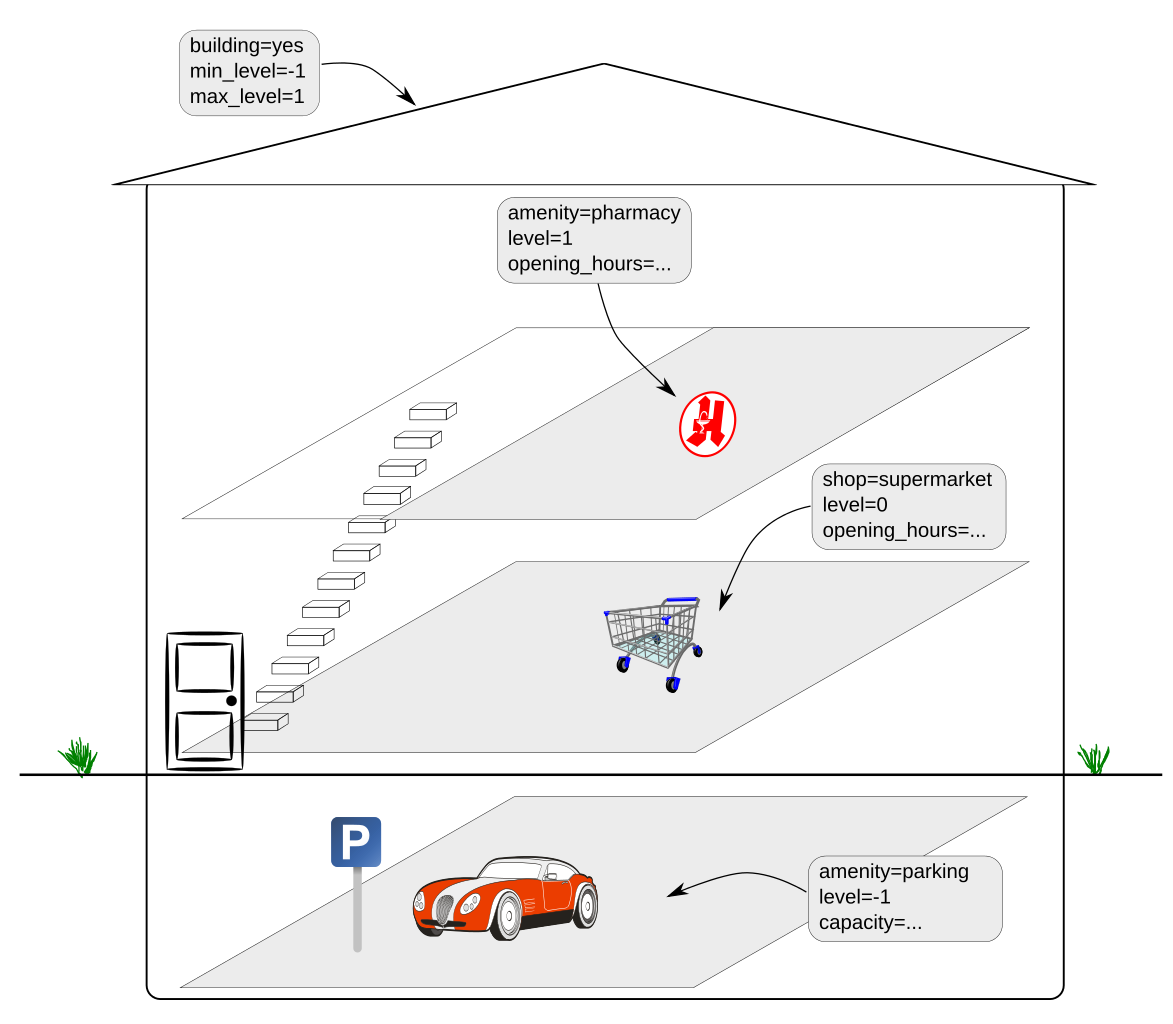
\includegraphics[width=.5\linewidth]{img/28a-simple_poi.png}}\hfill
                    \subfloat[\label{obr28b}]
                    {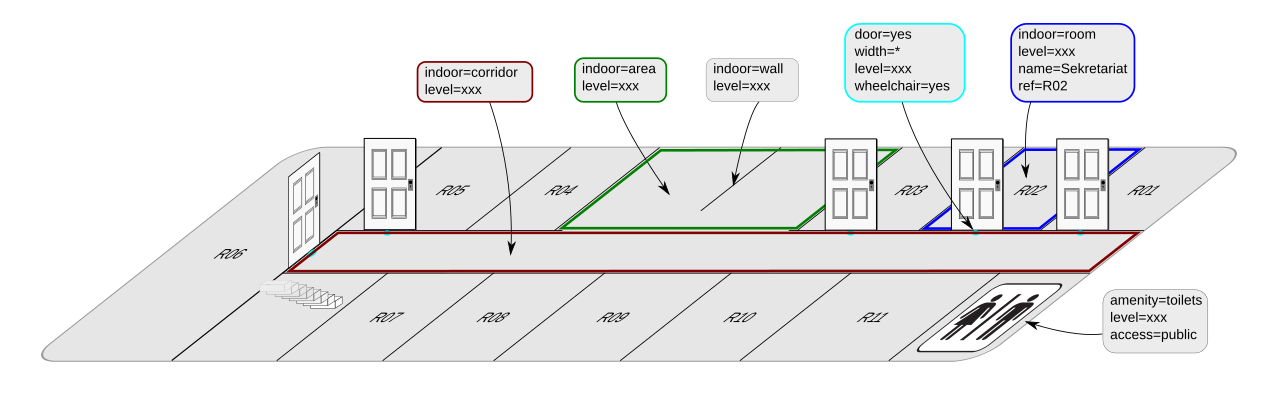
\includegraphics[width=.5\linewidth]{img/28b_elements.png}}

                    \caption{Jednoduché tagování bodů zájmu (a); detailní tagování místností (b)\cite{zdroj52}}
                    \label{obr28}
                    \end{figure}
                    

Pro jednoduché mapování bodů zájmu tedy navrhuje pouze přidat na obrys budovy tagy \texttt{min\_level=*}~a \texttt{max\_level=*}, které určí všechna patra budovy. Jednotlivé uzly uvnitř pak mají pouze nastavený \texttt{level=*}. ~Patra by měla korespondovat s~označením patra v~budově. Typicky \texttt{level=0}~znamená přízemí, ale nemusí tomu tak být. Pokud v~budově některé patro chybí, může to být označeno tagem \texttt{non\_existent\_levels=*}. ~Zcela odebírá nutnost používání relací, ale nezabraňuje jejich využití pro seskupení budovy a patra.

Navrhuje komplexnější mapování vnitřních prostor pomocí tagu \texttt{indoor=*}, například pokoj \texttt{indoor=room}~má implicitně stěny, zatímco chodba \\ \texttt{indoor=corridor} či jiná plocha~\texttt{indoor=area}~stěny nemá. Stěny lze také doplnit samostatně pomocí \texttt{indoor=wall}. Tak je možné pokrýt celé území patra a modelovat vše dle potřeby. K~označení čísla místnosti slouží tag \texttt{ref=*}, název klasicky \texttt{name=*}.

Spojení mezi patry je navrženo plochou, která se rozkládá přes více pater (např \texttt{level=0}-3). Každé patro je pak napojeno průchodem (\texttt{door=yes}~+ \texttt{level=0}). Routování je tedy umožněno přes všechny dotyky ploch beze stěn a též všemi průchody.

Dodatečné informace o~patru je možné zadávat k~obrysu patra s~tagem \texttt{indoor=level}, tam lze snadno propojit číslo patra \texttt{level=*}~s~jeho pojmenováním \texttt{name=*}, výškou \texttt{height=*}~a potažmo dalšími 3D vlastnostmi.

Ve výškových budovách se často rozložení chodeb, dveří a dalších prvků opakuje. I~na to autoři mysleli. Každý indoor prvek, který má definováno patro, může mít i tag \texttt{repeat\_on=*}, který značí patra, ve kterých je jeho úplná kopie. (Zde došlo v~průběhu psaní práce ke změně -- tag \texttt{level=*}~musí být přítomen vždy.)

Metodika se díky jednoduchosti ujala, ale ještě není považována za finální a tedy ani nezačal proces hlasování. V~první půlce roku 2015 vytvořil uživatel Panier Avide prohlížeč postavený na Overpass API -- \href{http://openlevelup.net}{openlevelup.net}. Indoor editor vznikl v~době dokončování této práce.

K~dipozici na: \href{http://wiki.osm.org/Simple\_Indoor\_Tagging}{wiki.osm.org/Simple\_Indoor\_Tagging}

\textbf{Naše hodnocení:}~Tento návrh~je vhodný k~následování, neboť respektuje~filozofii OSM s~možností postupného zlepšování zmapovanosti. Nejlépe ze všech využívá existující architekturu a nevytváří komplikované relace. Místo striktního \uv{flexibilního} oddělení pater relacemi využívá faktu, že patra jsou zkrátka přirozená čísla a tedy je není třeba nikde zvlášť definovat.\\
Spojení pater přirozeně modeluje například výtahovou šachtu -- ovšem pro schodiště chybí možnosti informace o~vedení schodů.

\subsubsection{Poznámka k~tagu \texttt{level=*}}\label{poznuxe1mka-k-tagu-level}

V~závěru roku 2011 se s~poněkud nejistým procesem objevila stránka o~tagu \texttt{level=*}, nejdříve pouze odkazovala na návrhy, které ho využívaly. Ovšem při postupném doplňování se z~ní stala \uv{uznaná vlastnost}. Nejspíše je to dáno její jednoduchostí a tím, že tag je intuitivně používaný. V~současnosti má téměř 300 000 výskytů.

\subsection{Výsledná metodika pro indoor mapy}\label{vuxfdslednuxe1-metodika-pro-indoor-mapy}

Naše řešení v~principu přímo~vychází ze Simple Indoor Tagging, ale chceme navrhnout jakési jádro indoor tagování, které nechá větší volnost ve volbě indoor prvků. Zejména doplňujeme robustnější variantu modelu \texttt{level=*}~a \texttt{repeat\_on=*}~a adresujeme některé další potíže.

\subsubsection*{Budovy}\label{budovy}

\begin{itemize}

\item
  U~budov (\texttt{building=yes}) i částí budov (\texttt{building:part=yes}) se zachovává \texttt{min\_level=*}~a \texttt{max\_level=*}. Též případné \\ \texttt{non\_existent\_levels=*}.
\end{itemize}



                      \begin{figure}
                    
                    \subfloat[\label{obr29a}]
                    {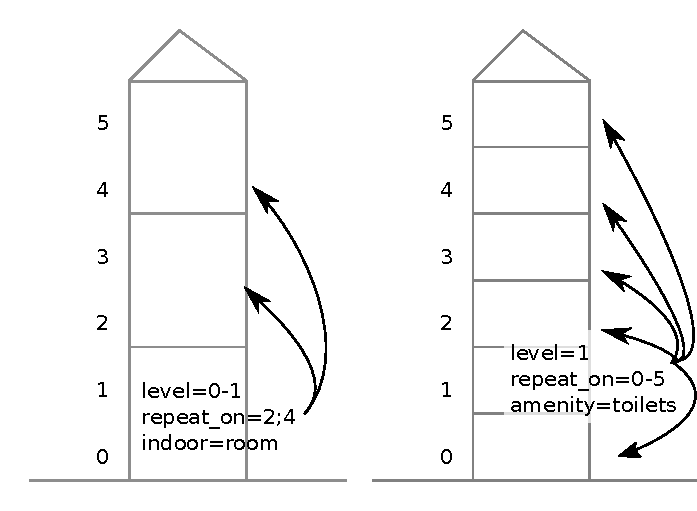
\includegraphics[width=.5\linewidth]{img/29a-nase-levelrepe.pdf}}\hfill
                    \subfloat[\label{obr29b}]
                    {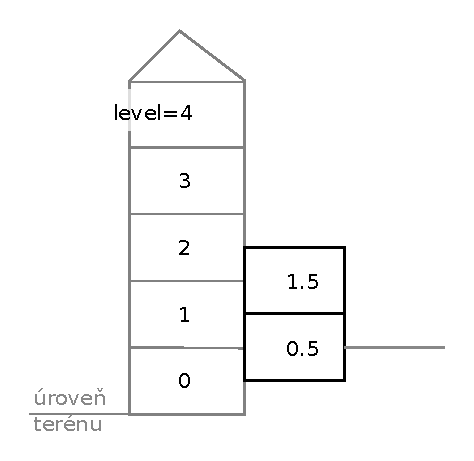
\includegraphics[width=.5\linewidth]{img/29b-nase-desetiny-level.pdf}}

                    \caption{Využití tagu level a repeat\_on (a); mezipatra pomocí desetinného čísla (b)}
                    \label{obr29}
                    \end{figure}
                    

\subsubsection*{Patra}\label{patra}

\begin{itemize}

\item
  Obtížnou situací v~OSM je, že formát \texttt{level=*}~musí být srozumitelný pro lidi,~aby ho dokázali intuitivně zadávat, a zároveň být samostatně srozumitelný i pro počítače, aby bylo možné patra seřadit, a tak vykreslit. Souhlasíme tedy se Simple Indoor, který navrhuje označování pater odpovídajícím číslem, např. v~budově s~patry S, P, 1, 2, bude patro \uv{S} odpovídat \texttt{level=-1} a patro \uv{P} \texttt{level=0}.
\item
  Označení pater je umožněno i v~desetinném formátu (viz obrázek \ref{obr29b}). To je vhodné pro tzv. mezaninové prostory a též třeba pro lepší vedení schodů. (Obrázek \ref{obr26a} na straně \pageref{obr26a})
\item
  Existence patra je implicitně předpokládaná, kdykoliv se v~něm vyskytuje libovolný prvek. Není tedy nutné vždy vytvářet budovu ani patro. Naopak, v~případě potřeby zaznačení více informací k~patru, využíváme obrys \texttt{indoor=level}~s~tagy \texttt{ref=*}, \texttt{name=*}, \texttt{height=*}~atd.
\item
  Každý prvek pro indoor musí mít tag \texttt{level=*}. V~syntaxi umožňujeme rozsah (0-2) pro rozpětí prvku přes více pater, např. výtahová šachta. Takový prvek se pak nachází v~celém intervalu, tedy i v~případných desetinných mezipatrech. Dříve využívaný výčet (0;1;2) se nedoporučuje, ale z~důvodu zpětné kompatibility ho interpretujeme jako diskrétní hodnoty.
\item
  Navíc každý prvek může mít tag \texttt{repeat\_on=*}, který značí jeho přesné opakování v~jiných patrech, včetně nastaveného rozpětí. (Viz obrázek \ref{obr29a}.) Syntaxe je doporučená výčtem (0;1;2). Využití rozsahu (0-2) je možné, ale znamená opakování ve všech patrech od minima s~\uv{násobky jedničky}. Tedy \texttt{repeat\_on=0}.5-3~ je ekvivalentní \texttt{repeat\_on=0}.5;1.5;2.5.
\item
  Rozsahy jsou pro oba tagy možné i v~záporných číslech, např. level=-1-5, či pro obě záporná čísla level=-4--1, vždy ovšem tak, že první hodnota je menší než druhá.
\item
  Přízemní patro není vyžadováno -- číslování je dáno číselným označením v~budově. Pro routing pak má význam informace,~ve kterém patře je uzel \texttt{entrance=main}~napojený na venkovní cesty.
\end{itemize}

\subsubsection*{Místnosti a chodby}\label{muxedstnosti-a-chodby}

\begin{itemize}

\item
  Chodby je nově možné tagovat jako klasickou cestu \texttt{highway=footway}. Považujeme totiž za zásadní dodržovat filozofii OSM -- mapovat od jednoduchého k~přesnějšímu. V~tomto je Simple Indoor příliš důkladný a rovnou nutí tvořit plošné vnitřní prostory.
\item
  Kromě chodeb se často vyskytují i jakási nádvoří či atria. Ty je vhodné otagovat plošnou komunikací,~jak je v~OSM zvykem; \texttt{highway=footway}~+ \texttt{area=yes}.
\item
  Navrhujeme oddělit primárně~průchozí oblasti (chodby), které budou značeny standardní komunikací, a primárně neprůchozí (místnosti), které budou značeny \texttt{indoor=*}~prvky dle Simple Indoor.
\item
  Místnosti je možné značit jako uzly nebo jako plochy pomocí \texttt{indoor=*}~či třeba pouze dveře \texttt{door=yes}. Opět dle filozofie od jednoduchého k~přesnějšímu. Dle možností je vhodné doplnit tag \texttt{ref=*}~či \texttt{name=*}.
\item
  Schody navrhujeme značit standardně \texttt{highway=steps}, typicky s~rozsahem přes více pater \texttt{level=0}-1. Aby se určilo, kde je začátek a konec, navrhujeme využít orientace cesty s~tím, že směr povede od nižšího patra k~vyššímu -- tedy šipka míří do kopce. Totéž platí pro libovolné cesty, které jsou vedeny přes více pater.
\end{itemize}

\subsubsection*{Shrnutí}\label{shrnutuxed}

Díky zjednodušení je možné využívat všechny prvky běžné v~OSM světě, pouze s~přidáním tagu \texttt{level=*}. Obrysy budovy jsou vhodné pro zobrazení ve webových mapách a umožňují i navigaci a geocoding v~budově. Zachována je i kompatibilita s~metodikou Simple 3D.

Pro konzumenta dat stačí v~OSM hledat všechny prvky s~tagem \texttt{level=*}~a \texttt{min/max\_level=*}, následně už je možné vytvořit uživatelsky přívětivý přepínač pater a zobrazovat jen relevantní data. Zde podotýkáme, že indoor prohlížeče z~principu musí fungovat na vektorových datech, neboť vyžadují vykreslování v~prohlížeči. Adepti na vektorové prohlížeče jsou technologie Mapbox GL, OSMBuildings JSON či mobilní aplikace typu Maps.me a Osmand.

Klasické 2D mapy jsou většinou předgenerované obrázkové dlaždice. Díky využívání tagů běžných komunikací jsou ovšem tyto vykresleny, a tak je většinou zachována informační hodnota i pro ně.

Editory pro toto schéma zatím neexistují a využívání rozsahů v~tagu \texttt{level=*}~nám brání snadno editovat v~editoru JOSM (na rozdíl od relací). Je tedy vhodné upravit stávající editory, aby schéma podporovaly. Úpravě iD se věnujeme v~další kapitole.

 \begin{figure}
	  \centering
      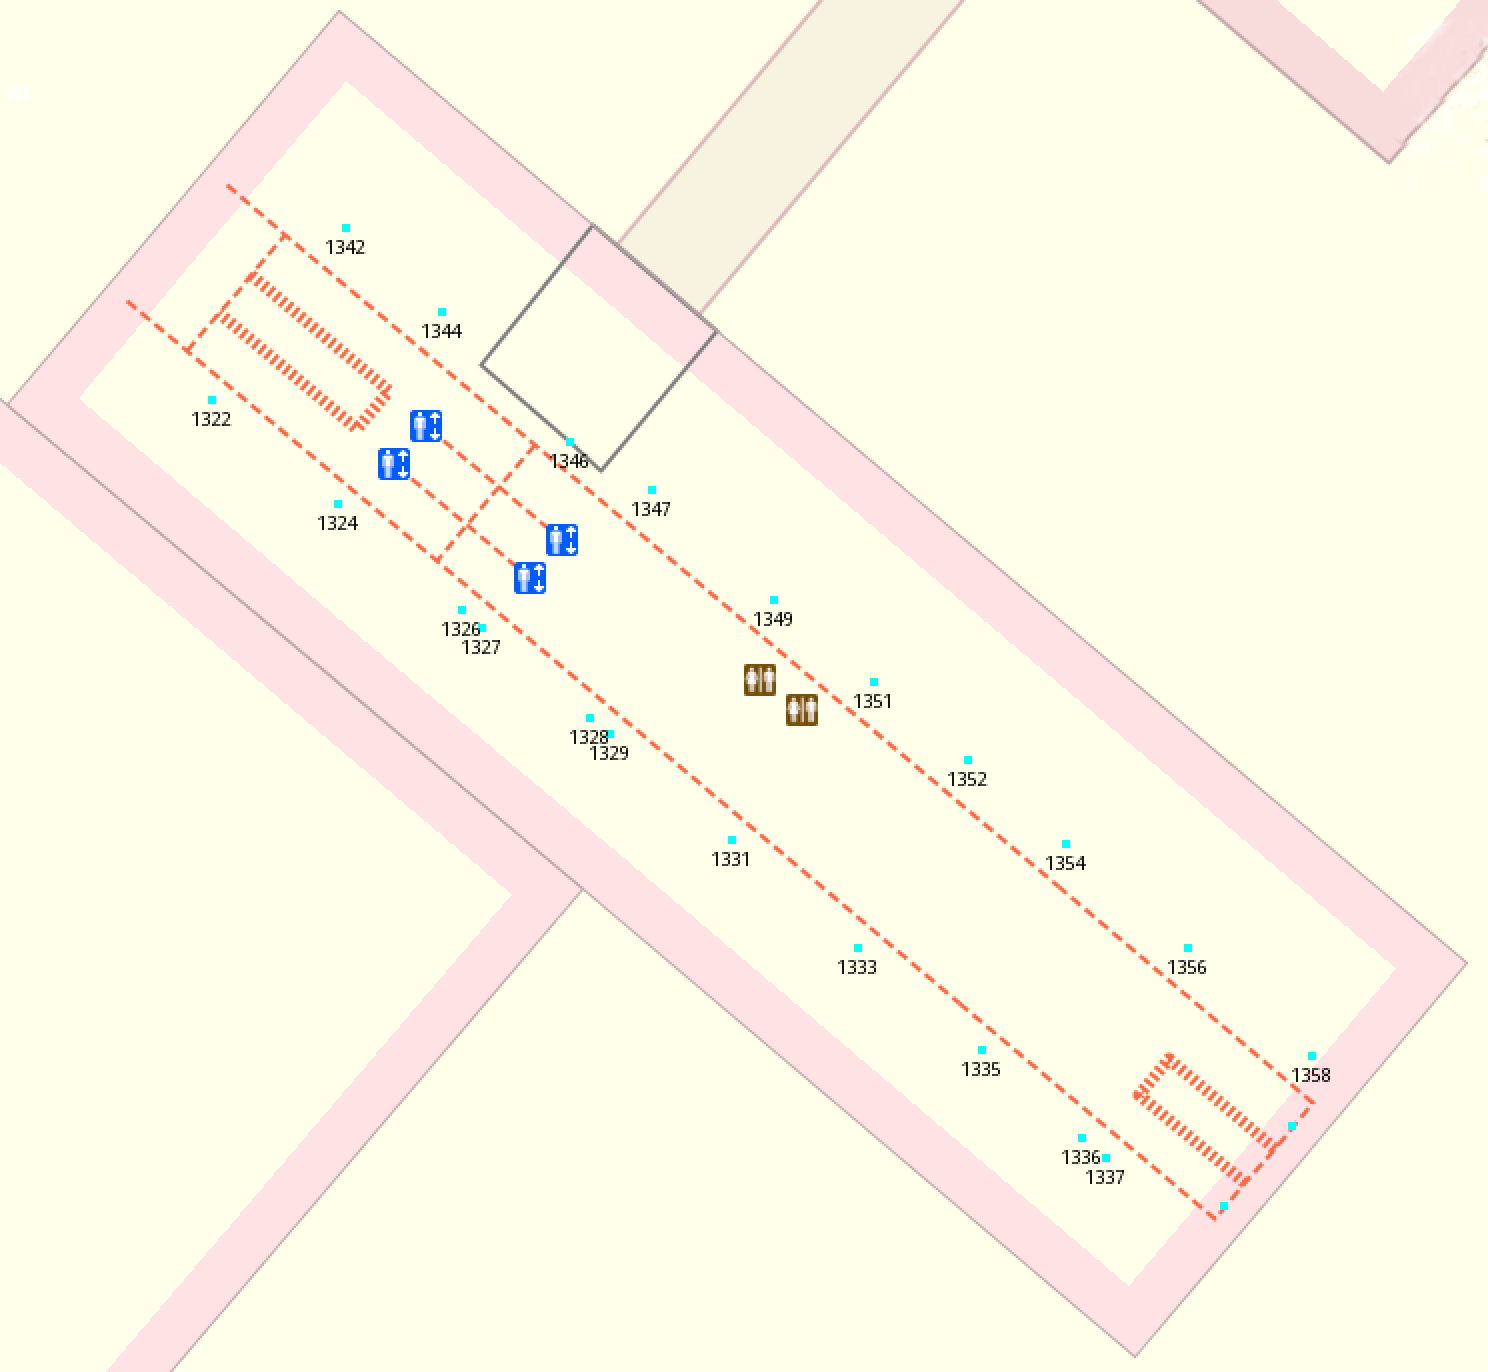
\includegraphics[width=.9\textwidth]{img/210-coreindoor-cvut-13.png}
      \caption{Zobrazení otagovaného patra 13 v~budově ČVUT (editor JOSM)}
      \label{obr210}
  \end{figure}

\section{3D}\label{d}

V~nedávné době také vznikla metodika pro vytváření 3D objektů nad OSM. Jednotlivým plochám přiřazuje mohutnost a výšku umístění nad povrchem. Navíc lze určit i vlastnosti jako barvu, typ střechy, materiál apod. V~praxi lze takto modelovat i složité objekty, ovšem nevýhodou je velké množství ploch, které musí být do databáze OSM přidáno.

Zobrazení v~prohlížeči technologií WebGL se věnuje open-source projekt \href{http://osmbuildings.com}{osmbuildings.com}~a komerční projekt \href{http://f4map.com}{f4map.com}.

 \begin{figure}
	  \centering
      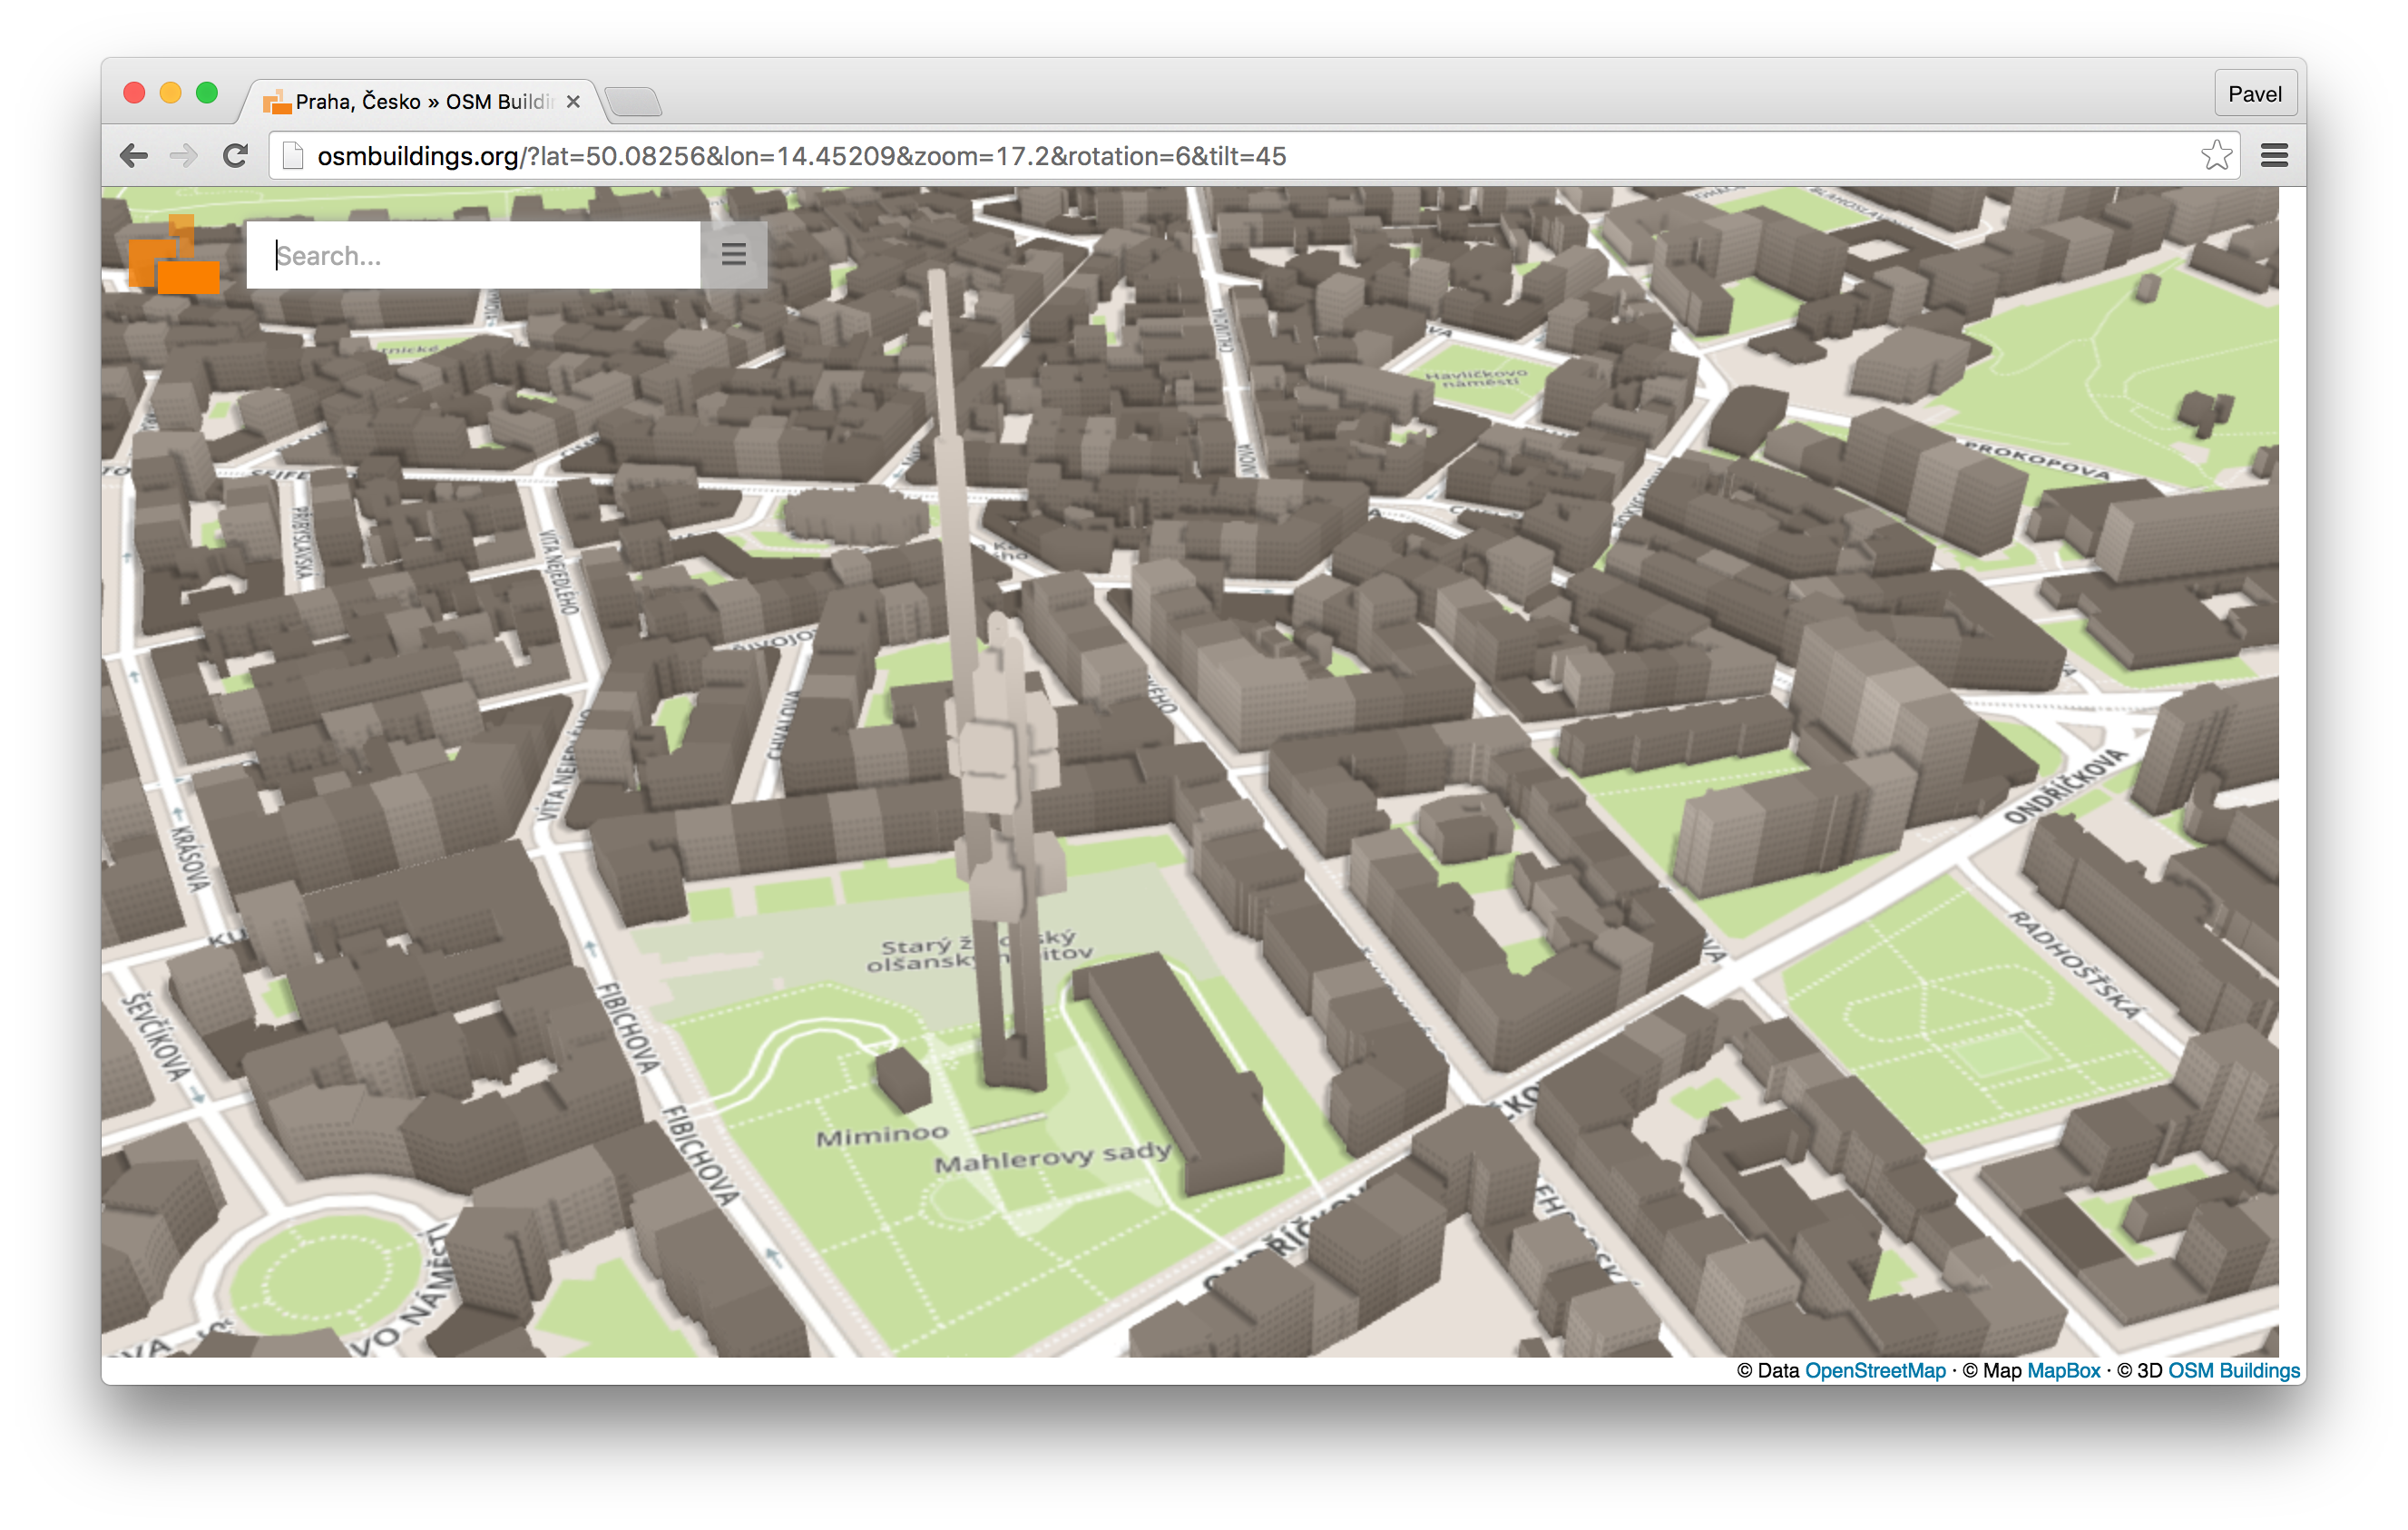
\includegraphics[width=\textwidth]{img/211-osmb.png}
      \caption{Zobrazení Žižkovského vysílače v~3D prohlížeči OSMBuildings}
      \label{obr211}
  \end{figure}



\chapter{Úprava editoru iD}\label{uxfaprava-editoru-id}

V~předchozí kapitole jsme položili důkladný úvod do architektury OSM, shrnuli předchozí návrhy~a navrhli novou metodiku pro indoor mapy. Tato kapitola pojednává o~implementaci této metodiky do editoru iD. Bylo třeba nastudovat pokročilou knihovnu d3.js, velmi sporou dokumentaci iD-core a pochopit jeho fungování z~kódu a debugingu. Po návrhu uživatelského rozhraní mohla začít implementace v~podobě přidání ovládacích prvků pro indoor mód a úpravy vykreslovacího enginu. Nakonec bylo možné sepsat pull request~do GitHub repositáře tohoto projektu a zasadit se o~jeho začlenění.

\section{Popis editoru a technologií}\label{popis-editoru-a-technologiuxed}

O~editoru jsme se již rozepsali~v~kapitole 2.2. Shrňme nyní, že se jedná o~webový editor postavený na několika technologiích z~rodiny HTML5. Cílí na začátečnickou skupinu uživatelů,~a proto má propracované jednoduché uživatelské rozhraní. Integrační a jednotkové testy jsou postavené na frameworku Mocha.

Pro úpravu bude zásadní vlastnost též filtrování zobrazených prvků dle kategorií, tzv. Features.

\subsection{Vizualizační knihovna d3.js}\label{vizualizaux10dnuxed-knihovna-d3.js}

Knihovna Data-Driven Documents (\href{http://d3js.org}{d3js.org}) se zabývá navázáním datových polí (arrays) na objektový model HTML dokumentu (DOM). Pro přídání a odebrání prvků do pole definuje enter \& exit transitions, které deklarativně určují,~co se při dané operaci~děje. Dokumentace knihovny je důkladná a díky své oblíbenosti lze najít i mnoho dalších zdrojů.

API knihovny je podobné známému jQuery, bez navázání dat můžeme říci, že totožné. Zde selektor a mutační funkce:

\begin{lstlisting}[language=javascript]
d3.selectAll("p").text("Hello")
\end{lstlisting}

Síla knihovny se ukáže při navázání dat, následně totiž můžeme do mutačních funkcí místo hodnot uvádět funkce. Při změně dat na stejném selektoru se pak automaticky provedou operace za enter()~funkcí, zde přidání odstavce a nastavení jeho textu dle datové hodnoty.

\begin{lstlisting}[language=javascript]
d3.select("body").selectAll("p")
   .data([4, 8, 15, 16, 23, 42])
   .enter().append("p")
    .text(function(d){ return "I'm number "+d+"!"; })
\end{lstlisting}


Základ je tedy jednoduchý, ale pro zápis animací a složitějších vnořených struktur vyžaduje jistý cvik. Abstrakce objektového modelu jako data je velmi užitečná a hodí se nejen pro vykreslení dat v~mapě, ale i některých ovládacích prvků.

\subsection{Architektura iD}\label{architektura-id}

Autoři na počátku zvolili\cite{zdroj53}~vykreslování dat pomocí inline SVG -- zápis vektorové grafiky~pomocí XML, které je možné přímo inline~vložit do HTML DOM. Velkou výhodou pak je, že SVG DOM generuje události jako HTML objekty, lze ho stylovat pomocí klasických selektorů CSS3 a lze ho pochopitelně vytvářet stejně jako HTML DOM. Přesně tyto výhody daly za vznik i knihovně d3.js pro abstrakci vizualizací nejen nad SVG.

Druhá možnost by byla používat tzv. HTML canvas, jehož vykreslení je mnohokrát rychlejší, nenáročné na paměť a podporované i staršími prohlížeči. Ovšem v~tu chvíli by autoři museli programovat všechny věci ohledně grafického enginu sami. S~SVG naopak využili grafické jádro prohlížeče. Volba padla zejména pro větší flexibilitu a snadnější vývoj.

Kromě samotné knihovny d3.js využívá iD i několika rozšíření: d3.xhr()~pro posílání AJAX požadavků, d3.dispatch()~pro volání callback funkcí dle návrhového vzoru observer\cite{zdroj54}, d3.geo.path()~pro generování SVG linek dle souřadnicí a zadané projekce a d3.behavior.zoom()~pro zoomování a posouvání mapy pomocí CSS3 transformací.

\subsection{Core architektura}\label{core-architektura-1}

Jádro editoru se týká zejména datového modelu postaveného nad OSM XML API. Využívá několik velmi hezkých vlastností a je velmi důkladně otestováno.

Entity odpovídají základním prvkům OSM: iD.Node, iD.Way~a iD.Relation. Jako jediné v~projektu využívají dědičnosti, a to od iD.Entity. Lze tak přistupovat k~vlastnostem ID, tags a dalším dle typu. Díky odlišnému jmennému prostoru pro identifikátory OSM typů zavádí jednotný jmenný prostor identifikátorů, kde prefixuje číselné ID prvním písmenem typu, např. n123, w42, r30.

Velmi chytře navrženou částí je implementace historie; podobá se verzovacímu systému Git. Každá entita je po vytvoření neměnná (immutable) -- to znamená, že tu konkrétní instanci objektu už nelze změnit. Entity jsou sdruženy v~neměnném grafu, který ukazuje na jednotlivé neměnné objekty. Při \uv{úpravě} jedné entity je tak vlastně vytvořena nová entita s~upravenými vlastnostmi a vytvořen nový graf, který ukazuje na všechny původní entity a jednu novou.

Graf tedy odpovídá Git stromu a entity jednotlivým Git objektům. Tato implementace je velmi šikovná na funkci \uv{zpět} (undo) a nabízí dobrou abstrakci.

 \begin{figure}
	  \centering
      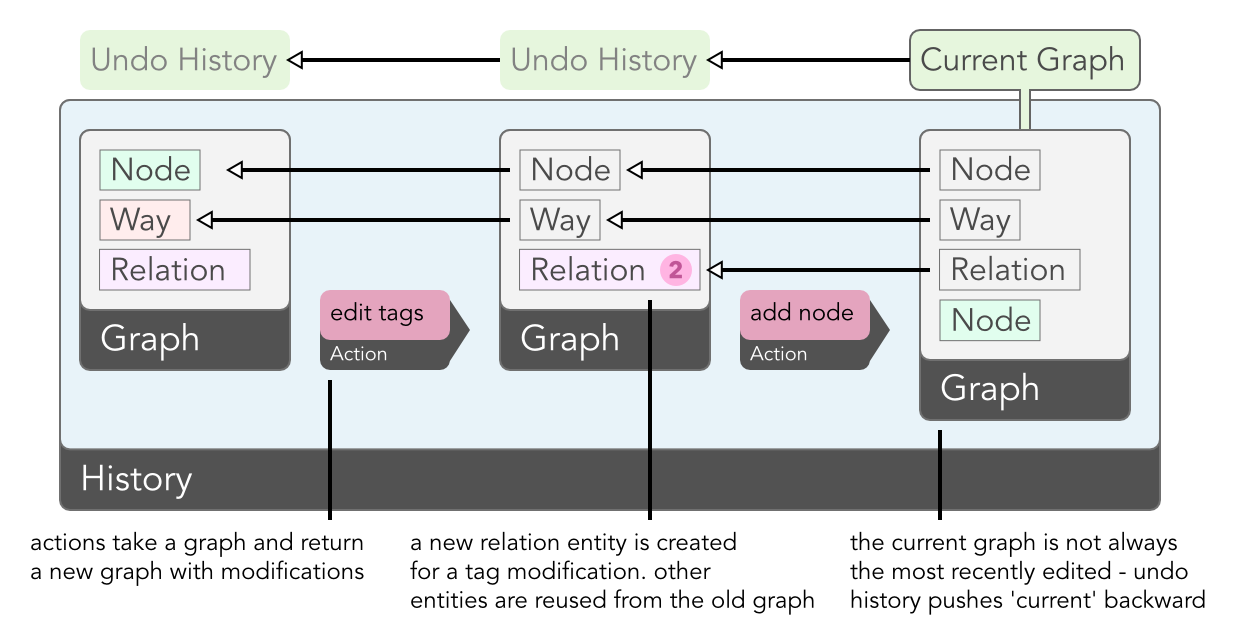
\includegraphics[width=\textwidth]{img/31-id-graph.png}
      \caption{Historie a graf jako neměnný objekt\cite{zdroj53}}
      \label{obr31}
  \end{figure}

Datový model nabízí několik dalších šikovných funkcí:

\begin{itemize}

\item
  iD.Difference(g1,g2)~-- vrací změněné prvky mezi dvěma grafy, což je potřebné pro vykreslení změn.
\item
  iD.Tree(g)~-- obalí daný graf datovou strukturou R-tree a následně umí efektivně vrátit entity ve zvolném souřadnicovém rámečku BBOX. Složitost vyhledání je O(logMn), maximální počet listů byl zvolen M=9.\\
  Příklad: 
\texttt{var features = tree.intersects(iD.geo.Extent([0, 0], [2, 2]), tree.graph());}
\item
  iD.Action()~-- abstrakce nad více operacemi na grafu; vytváří nový graf, který uloží do historie. Např. při smazání cesty se odeberou i všechny její uzly. iD.Operation()~pak abstrahuje akci na operaci proveditelnou tlačítkem či klávesovou zkratkou a hlídá, jestli je možné v~danou chvíli akci provést.
\item
  iD.Mode(), iD.Behaviour()~-- základní mód je prohlížení mapy a tlačítky je možné zvolit tři módy pro přidávání uzlů, cest a ploch. Módy definují chování jako například zvýraznění po najetí myší na prvek, apod. (Poznámka: vyvíjený Indoor mód není módem v~tomto \uv{core} smyslu)
\item
  Samotné vykreslování SVG zajišťuje iD.Map, která implementuje příslušné: iD.svg.Points, iD.svg.Vertices, iD.svg.Lines~a iD.svg.Areas.
\end{itemize}

\section{Návrh uživatelského rozhraní}\label{nuxe1vrh-uux17eivatelskuxe9ho-rozhranuxed}

\subsection{První iterace}\label{prvnuxed-iterace}

Uživatelské rozhraní bylo třeba vyvíjet v~několika iteracích a výsledky testovat. První lo-fi prototyp byl proveden na papíře a zde je prezentován pomocí softwaru Blasamiq Mockups (obrázek \ref{obr32}).

 \begin{figure}
	  \centering
      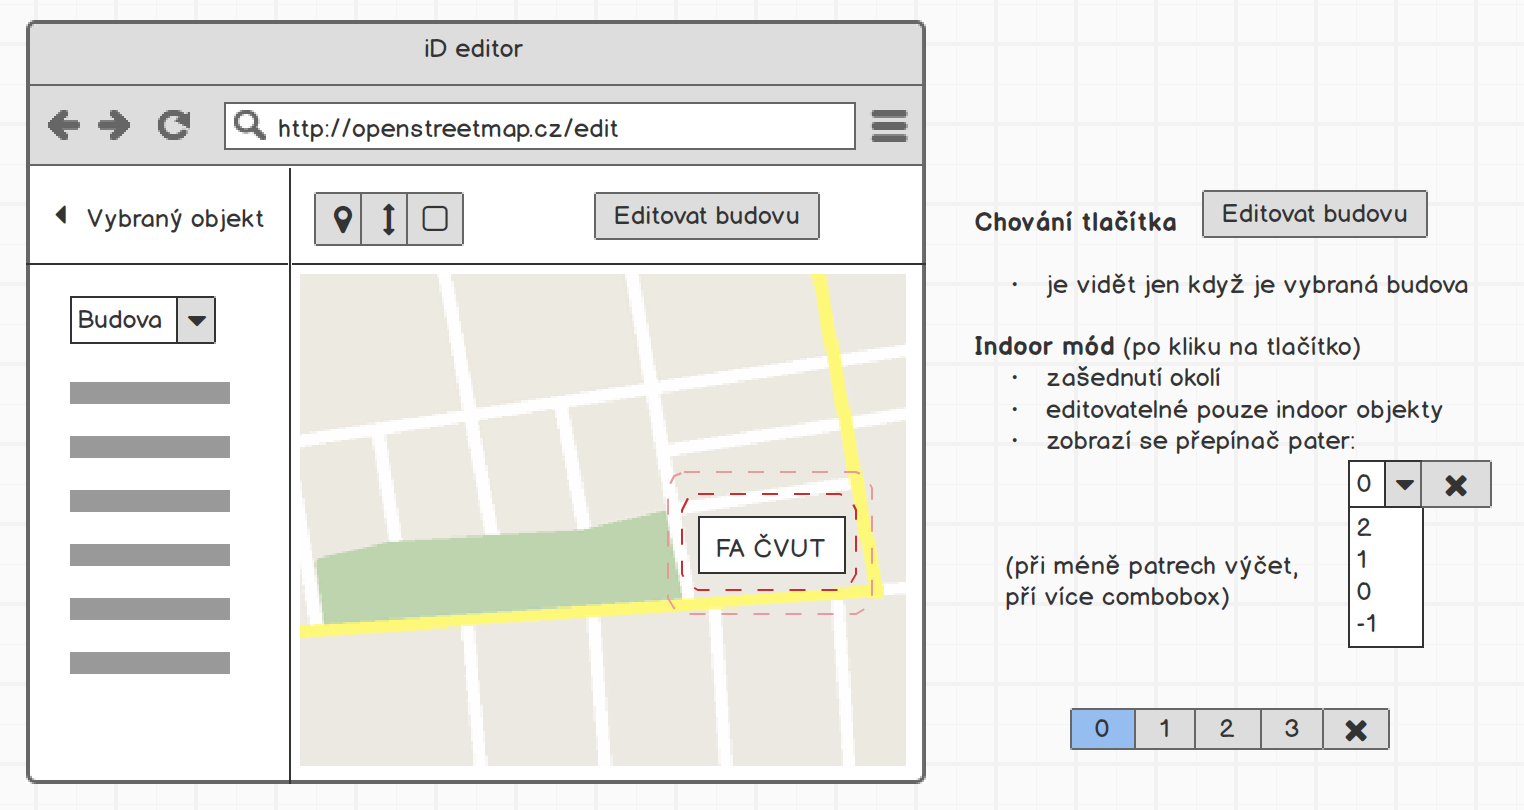
\includegraphics[width=\textwidth]{img/32-id-navrh-ui-1.png}
      \caption{První návrh uživatelského rozhraní včetně popisu interakcí}
      \label{obr32}
  \end{figure}

Následně proběhlo několik diskusí a testů a rozhodli jsme se návrh přehodnotit.

\subsection{Druhá iterace}\label{druhuxe1-iterace}

Pro uživatele by byla~nešikovná nutnost vybrat budovu, ačkoliv to je implementačně snazší (přepínač pater nabízí pouze patra pro konkrétní budovu). Navíc v~naší metodice umožňujeme tvorbu \texttt{level=*}~prvků i bez ohraničující budovy, což by se muselo adaptovat.

\begin{itemize}

\item
  Tlačítko se tedy bude jmenovat \uv{Indoor mód} a bude se ukazovat vždy při vybrané budově či prvku s~\texttt{level=*}. Indoor mód se zapne přesně do patra vybraného prvku.
\item
  Přepínač pater bude aktivní napříč celou aplikací -- to také intuitivně odpovídá umístění v~záhlaví, nikoliv u~zvoleného prvku. Nabízet se tedy budou všechna dostupná patra ve výřezu.
\item
  V~indoor módu se nyní schovají všechny nesouvisející prvky, aby uživatel věděl,~čeho se týká jeho editace.
\item
  Vyznačení plochy budovy bylo rozšířeno i vně, aby ji bylo možné vybrat při plném pokrytí indoor plochami.
\end{itemize}

 \begin{figure}
	  \centering
      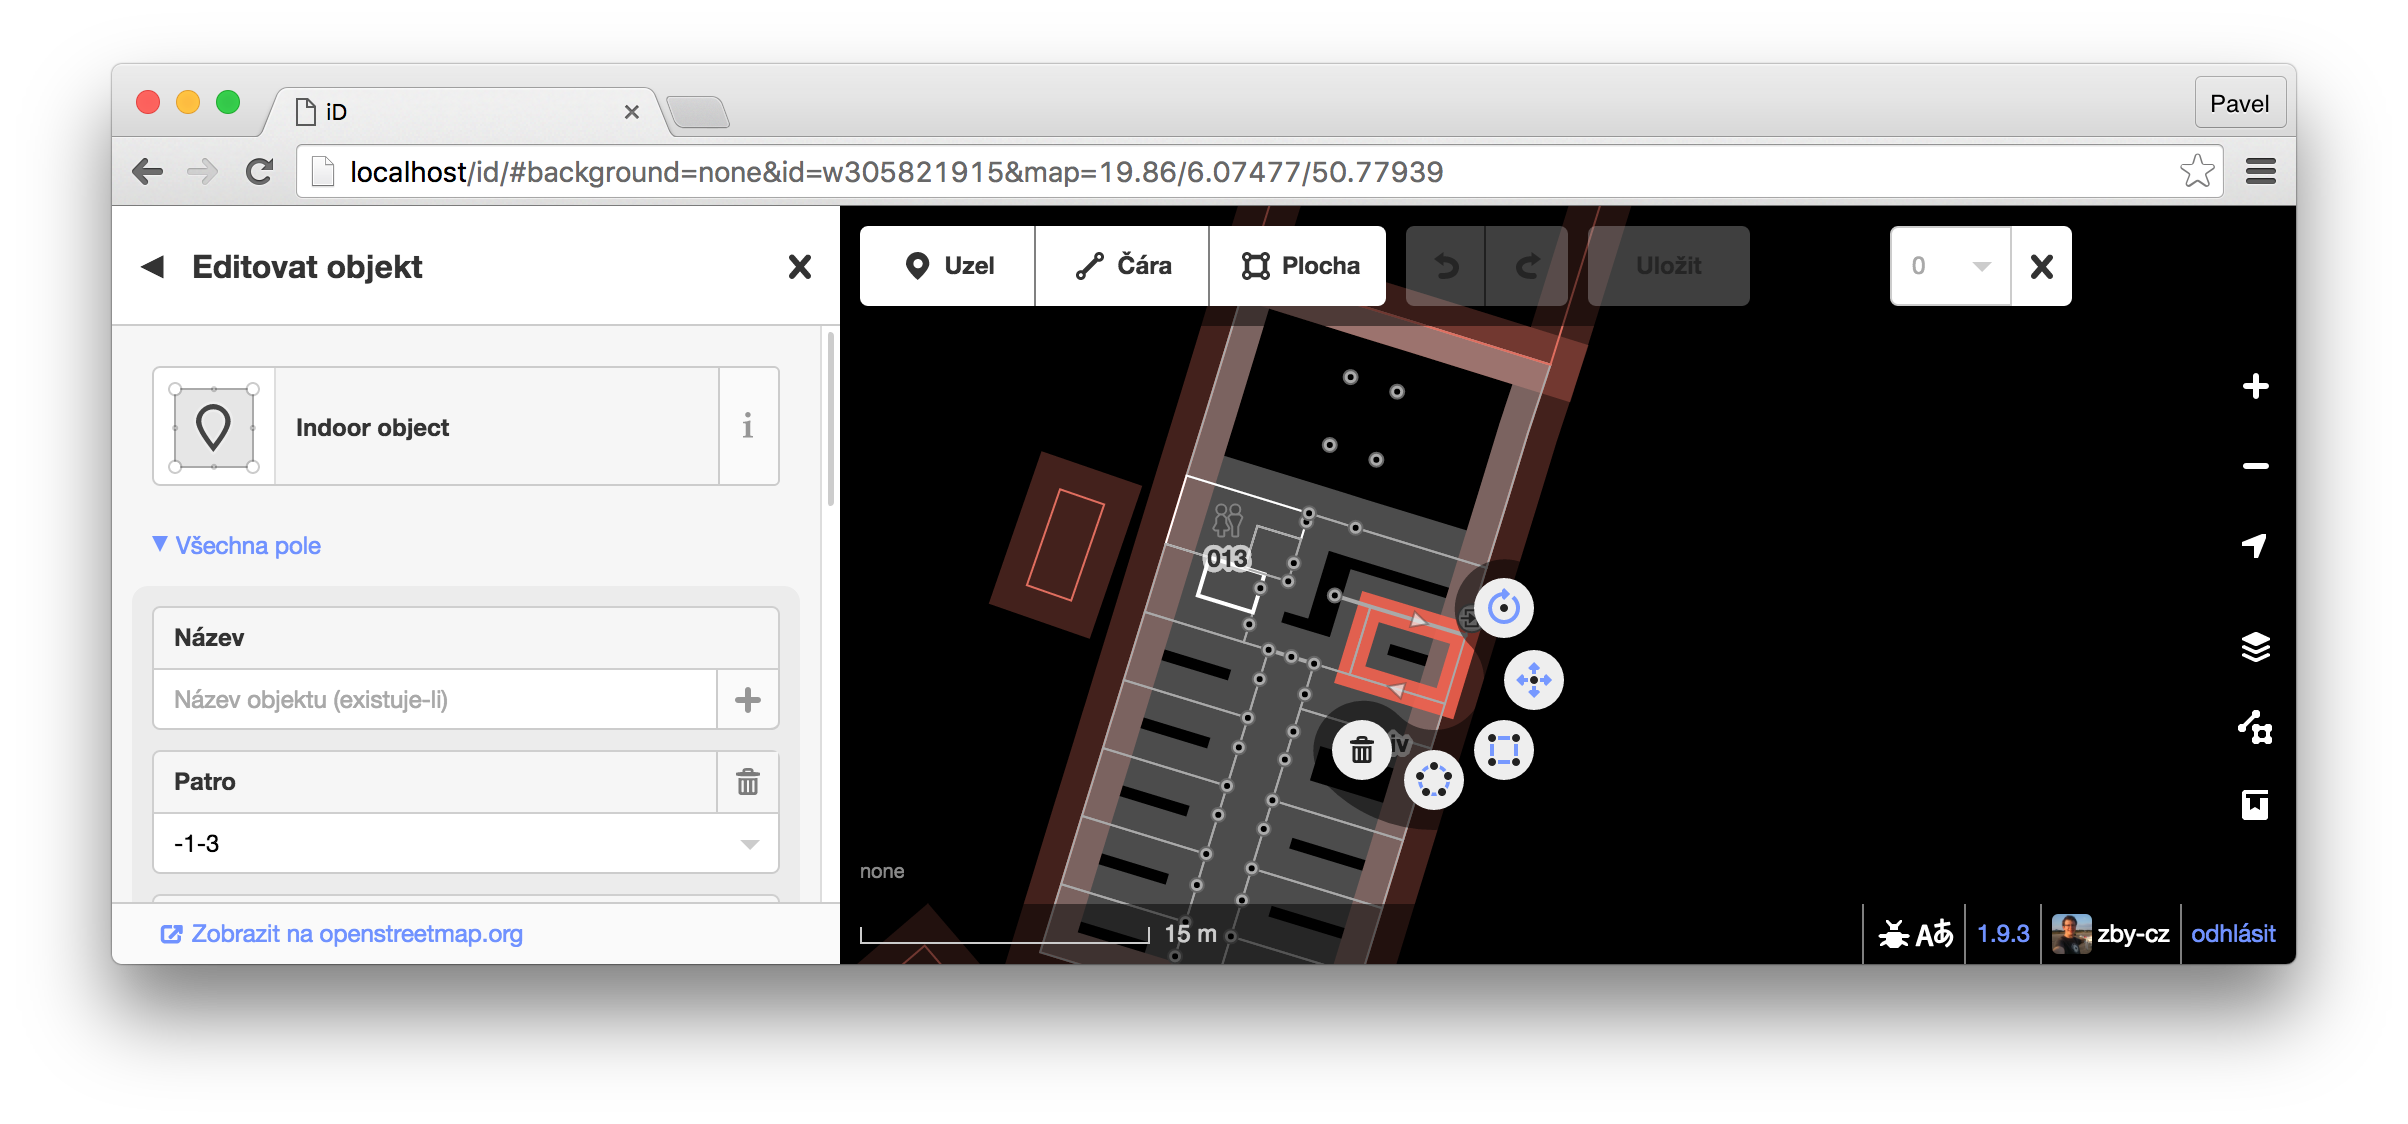
\includegraphics[width=\textwidth]{img/33-id-iterace-2.png}
      \caption{Upravený editor po druhé iteraci a zobrazené operace}
      \label{obr33}
  \end{figure}


                      \begin{figure}
                    
                    \subfloat[\label{obr34a}]
                    {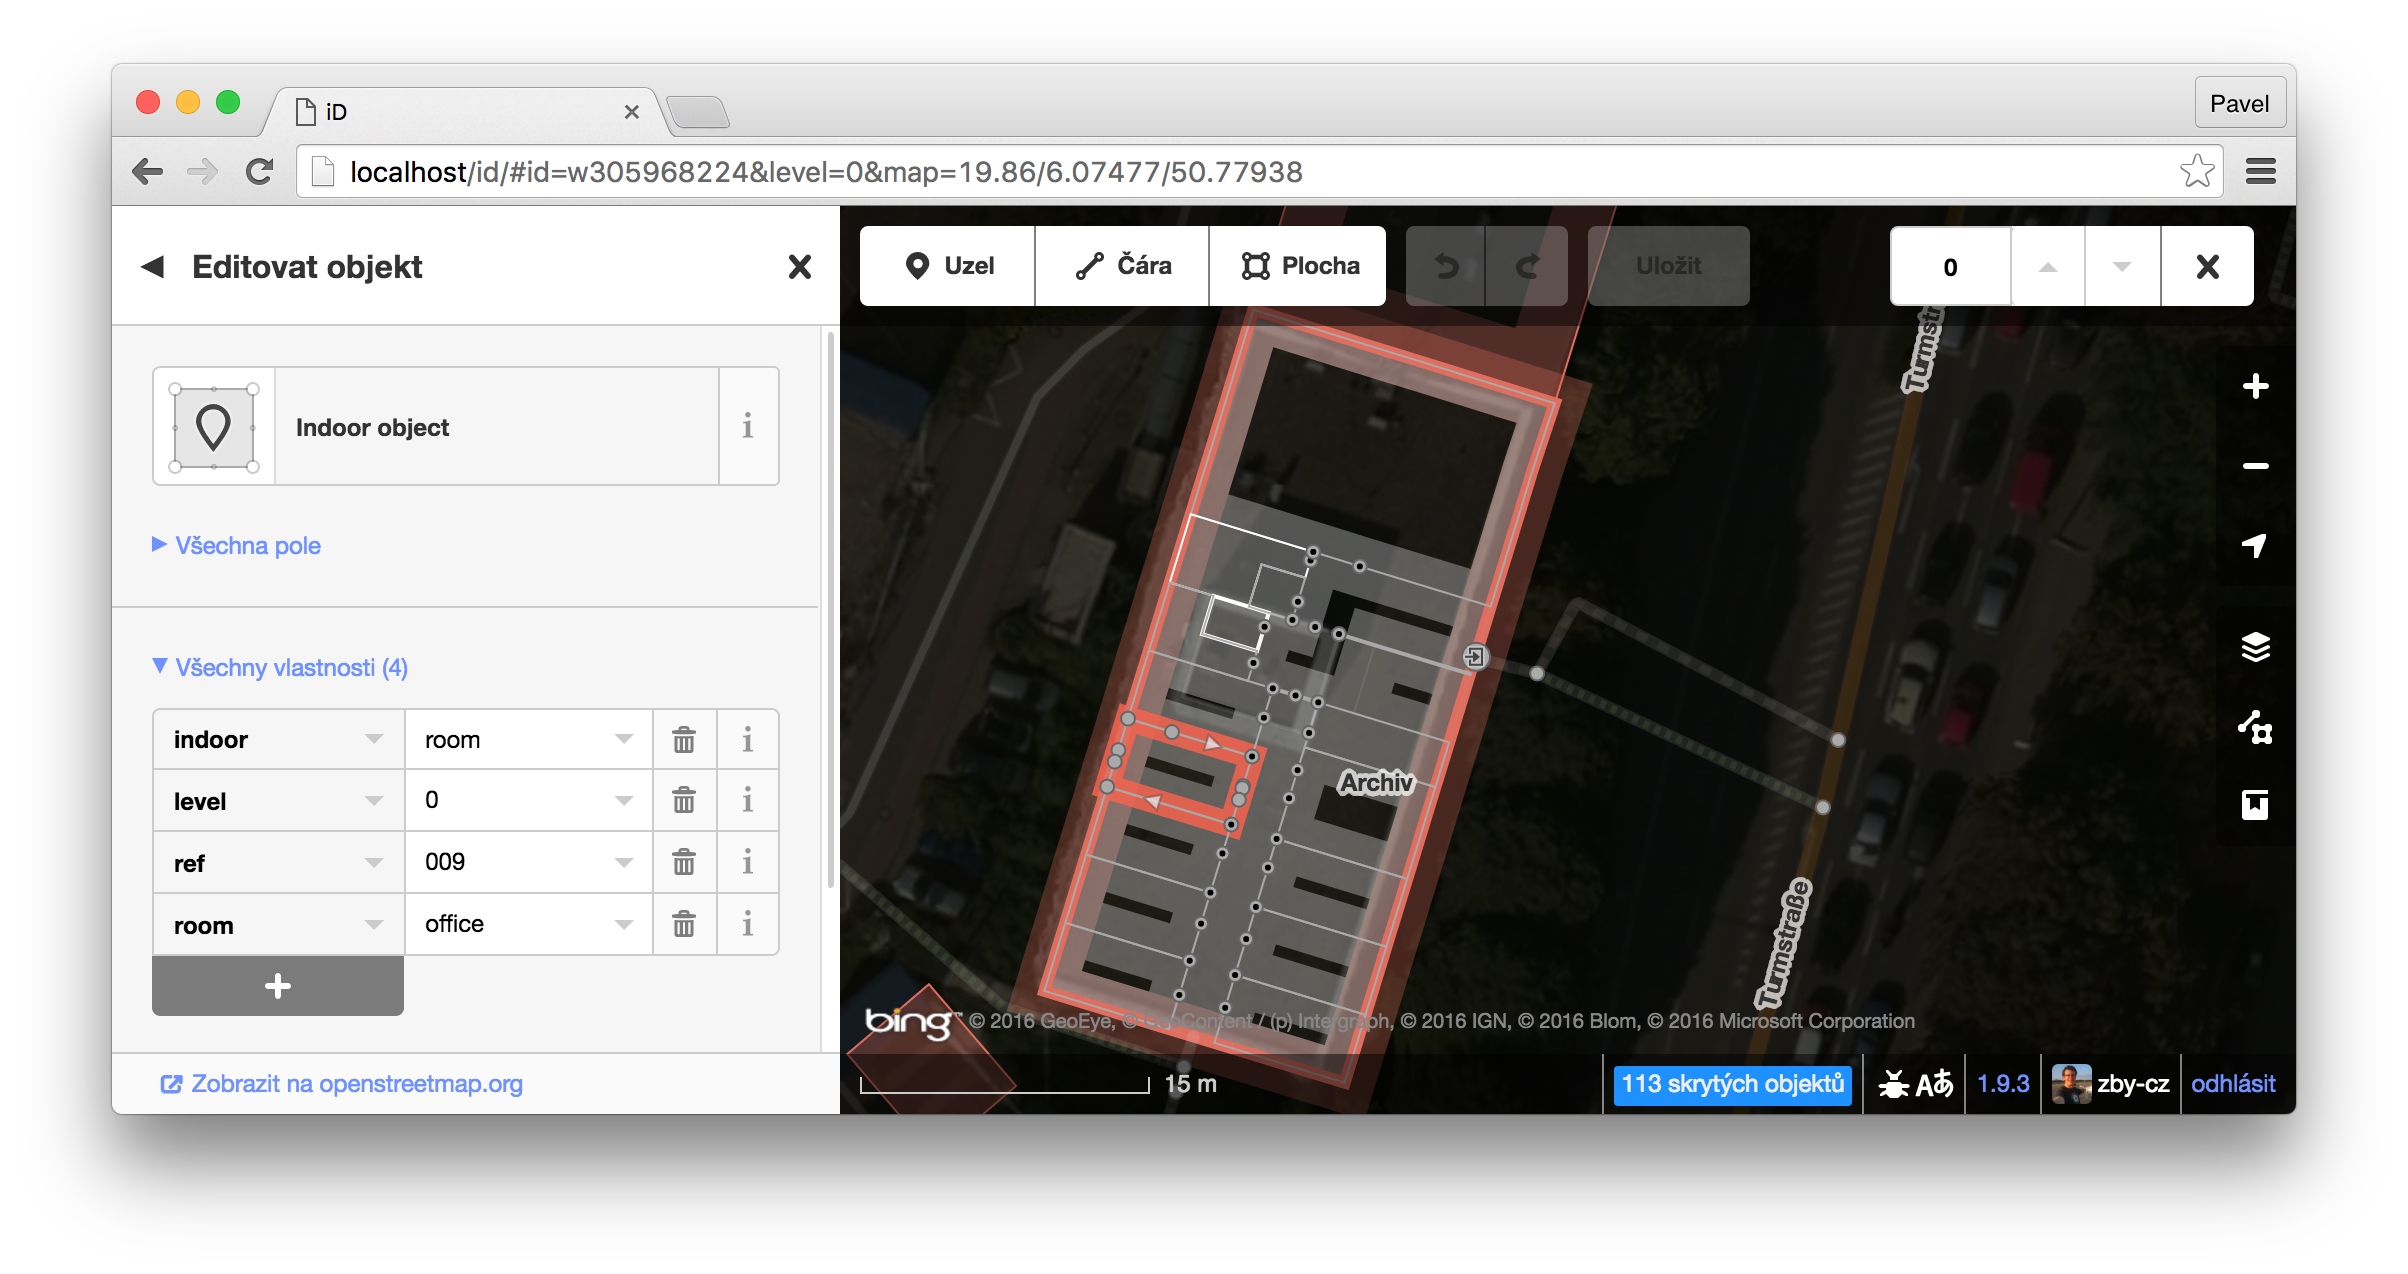
\includegraphics[width=\linewidth]{img/34a-id-iterace-3-4-kladne.png}}\hfill
                    \subfloat[\label{obr34b}]
                    {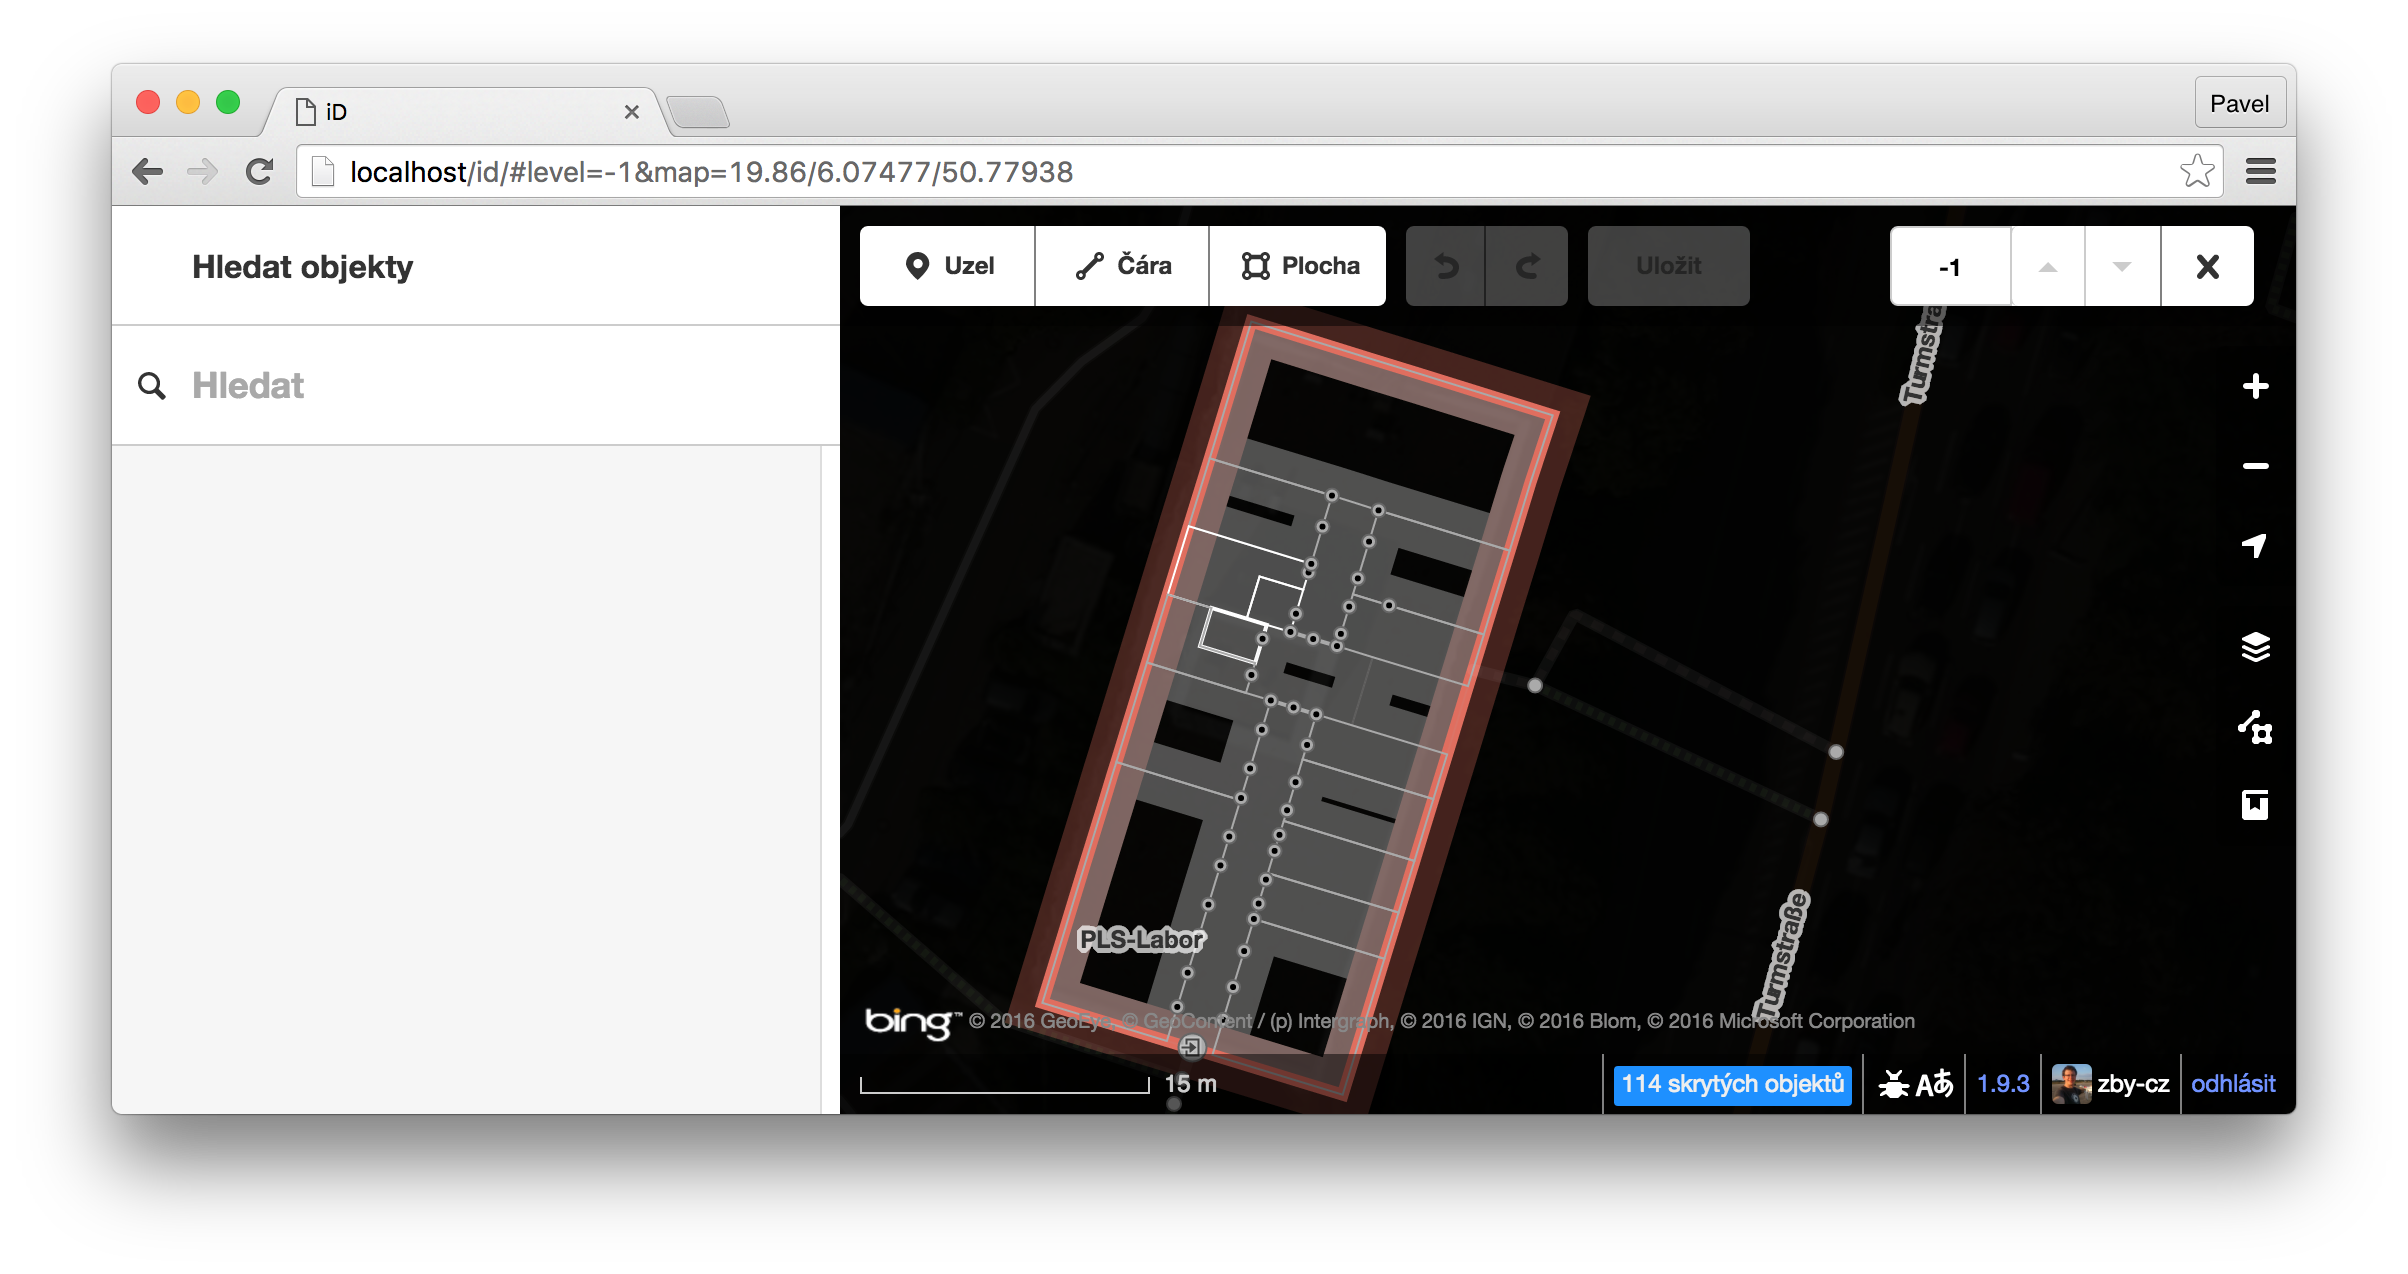
\includegraphics[width=\linewidth]{img/34b-id-iterace-3-4-patro-zaporne.png}}

                    \caption{Finální editor po čtvrté iteraci~v~patře 0 (a); a v~patře -1 (b)}
                    \label{obr34}
                    \end{figure}
                    

\subsection{Třetí a čtvrtá iterace}\label{tux159etuxed-a-ux10dtvrtuxe1-iterace}

Pro jednoduchost shrnujeme výsledky a obrázky po obou iteracích (\ref{obr34}), a tedy náš závěrečný editor. Více obrázků je k~dispozici v~další kapitole.

\begin{enumerate}

\item
  Pro uživatele bylo matoucí skrytí všech okolních prvků, ponechali jsme tedy všechny komunikace.
\item
  Aktivní ortofoto vrstvu jsme pouze utlumili, stejně tak všechny komunikace bez \texttt{level=*}. Při přechodu do záporných pater je pak obojí utlumeno podstatně více.
\item
  Pro lepší vnímání výšky zobrazujeme jen ty budovy, které mají příslušná patra (\texttt{building:levels=*}). Budovy s~\texttt{min/max\_level=*}~jsou navíc zvýrazněné, aby uživatel poznal, že do nich může mapovat.
\item
  Přepínači pater jsme přidali tlačítka pro zvýšení a snížení patra o~jedničku. Tlačítka jsme zvětšili a umístili vedle sebe, protože musí být dostupná, kvůli častému používání. Pro editor je tento přístup přirozenější než výběr z~existujících~pater, protože přirozeně vede uživatele k~tomu, aby v~novém patře začal tvořit.
\item
  Plochám \texttt{indoor=corridor}~a \texttt{indoor=area}, tedy těm beze stěn, jsme zeslabili ohraničení, neboť silnější ohraničení evokuje stěnu.
\item
  Informaci o~zvoleném patře jsme přidali do URL, pro možnost odkazování na konkrétní patro v~indoor módu.
\end{enumerate}

Čtvrtá iterace se týkala pouze drobných úprav přepínače.

\begin{enumerate}

\item
  Tlačítka pro zvýšení a snížení patra jdou přes desetinná patra, v~případě, že taková existují.
\item
  V~nabídce comboboxu~se zobrazují pouze ta patra, která jsou explicitně definovaná v~tagu \texttt{level=*}. Pomáhá to uživateli ve zjištění, která patra jsou zmapovaná.
\end{enumerate}

\section{Implementace}\label{implementace}

Bylo potřeba přidat ovládací prvek pro aktivaci Indoor módu a následnou volbu patra. Dále pak zajistit skrytí prvků v~jiných patrech.

Nejdříve se zdálo vhodné upravit třídu iD.map~v~místě, kde posílá všechny entity k~filtrování Features a dál k ~vykreslení SVG:

\begin{lstlisting}[language=javascript]
if (context.indoorMode()) {
 data = data.filter(function (entity) {
   return inRange(context.indoorLevel(), entity.tags.level)...;
 });
}
data = features.filter(data, graph);   // filtrov{' a}n{' i}
svgSurface.call(drawVertices, graph, data, filter, map.extent(), map.zoom()) ...
\end{lstlisting}



Ovšem záhy se toto řešení ukázalo jako nevhodné. Toto volání se provádí velmi často -- při každé události context.enter~(vybrání prvku, úprava atd.), při map.move~(posun mapy tzv. debounced na 400 ms) a dalších. Vykreslení pomocí d3.js je rychlé (vykreslí se jen DOM pro změny), Features využívá cachování. Ovšem náš přístup by při každém volání musel naparsovat \texttt{level=*}~tag pro všechny prvky a zjistit, zda se nachází v~rozsahu.

Bylo tedy třeba hledat jiné řešení. To jsme našli v~podobě již fungujícího filtrování Features. Logika je poměrně složitá, protože kromě skrytí prvků dle zaškrtnutých kategorií se zde provádí i tzv. autohide. Ten automaticky skrývá prvky v~případech,~kde by jich bylo příliš mnoho na čtvereční jednotku. Navíc jeden prvek může patřit i do více kategorií a je skryt,~pokud je skryta alespoň jedna z~nich.

Definovali jsme tedy kategorii indoor~a indoor\_different\_level, kterou bylo třeba při zapnutí indoor módu automaticky schovat:

\begin{lstlisting}[language=javascript]
defineFeature('indoor', function isIndoorOther(entity) {
  return !!entity.tags.level;
});
defineFeature('indoor_different_level', function isHiddenByLevel(entity, resolver, geometry) {
  return inRange(context.indoorLevel(), entity.tags.level) ... ;
});
\end{lstlisting}


Tím jsme využili mnoho stávající logiky a zároveň při vstupu do Indoor módu mohli i přirozeně vypnout nežádoucí Features.

Následně bylo třeba správné vykreslení uzlů s~vlastnostmi, skrývání uzlů v~cestě dle jejích vlastností, vynucení skrytí i pro nově přidané prvky a mnoho další vývojové i ladicí práce, která je dostupná ve zdrojových kódech.

Práci mimo jádro (tedy vykreslovací vzhledy, presets a další) zde nerozepisujeme, neboť není tak technicky náročná -- popis se nachází v~předchozí kapitole a samozřejmě je i k~nahlédnutí diff zdrojových kódů.

\section{Začlenění do projektu iD}\label{zaux10dlenux11bnuxed-do-projektu-id}

Naše úpravy proběhly na forku Git repozitáře. Po dokončení třetí iterace byl zaslán tzv. pull-request. Jedná se o~standardní formu jak na GitHubu nabídnout správci nějakého projektu začlenění nového kódu.

Pull request je k~dispozici na adrese \\ \href{https://github.com/openstreetmap/iD/pull/3097}{github.com/openstreetmap/iD/pull/3097}~a otisk ke stavu odevzdání v~příloze této práce a na CD.

Hlavní správce projektu, Bryan Housel, na něj reagoval ve smyslu, že se mu práce líbí a rád by ji~do projektu v~nějaké formě začlenil. Ovšem nejdříve bude třeba vymyslet,~jak lépe pojmout uživatelské rozhraní -- rád by,~aby tlačítko bylo dostupné stále, ale trochu méně nápadné.

Na dalším vývoji budeme spolupracovat i nad rámec této diplomové práce.

 \begin{figure}
	  \centering
      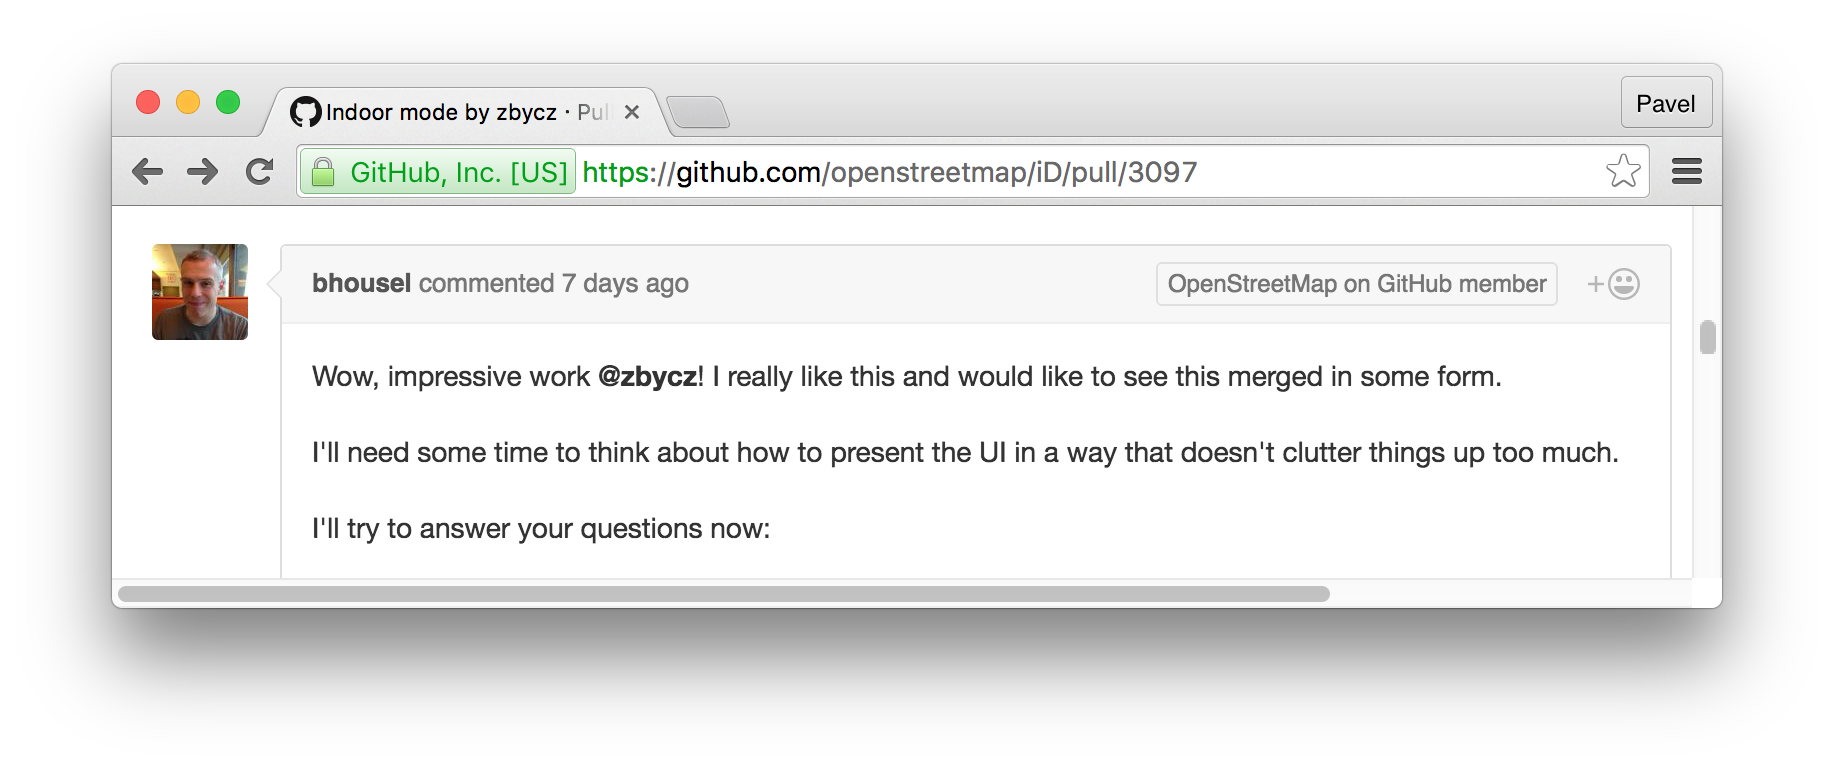
\includegraphics[width=\textwidth]{img/35-pull-req-comment.png}
      \caption{První komentář správce projektu\cite{zdroj56}}
      \label{obr35}
  \end{figure}



\chapter{Využití výsledků práce}\label{vyuux17eituxed-vuxfdsledkux16f-pruxe1ce}

Vytvoření dobré metodiky a editoru pro indoor mapy v~OSM jsou základní předpoklady pro to, aby se toto odvětví mohlo plně rozvinout. V~této kapitole prezentujeme některá zmapovaná~místa, navrhujeme indoor řešení pro veřejné instituce a zamýšlíme se nad možnou prezentací indoor mapy.

\section{Zmapovaná místa}\label{zmapovanuxe1-muxedsta}

Pro otestování naší výsledné metodiky jsme zmapovali,~s~hrubými detaily,~vnitřní plán dvou budov ČVUT (obrázek \ref{obr41a}) a stanici metra Dejvická (obrázek \ref{obr43a}). Tyto změny jsou k~dispozici v~databázi OSM a též na přiloženém CD.

Mnoho míst již bylo zmapováno pomocí metodiky Simple Indoor Tagging. Seznam je k~dispozici na stránce metodiky\footnote{\href{http://wiki.osm.org/Simple\_Indoor\_Tagging}{wiki.osm.org/Simple\_Indoor\_Tagging}}~a v~prohlížeči OpenLevelUp\footnote{\href{http://openlevelup.net}{openlevelup.net}}. Díky kompatibilitě obou metodik je možné tato místa prohlížet i v~upraveném editoru\footnote{K dispozici na stránce \href{http://openstreetmap.cz/edit}{openstreetmap.cz/edit}}, který je výsledkem této práce.


                      \begin{figure}
                    	  \centering
                    \subfloat[\label{obr41a}]
                    {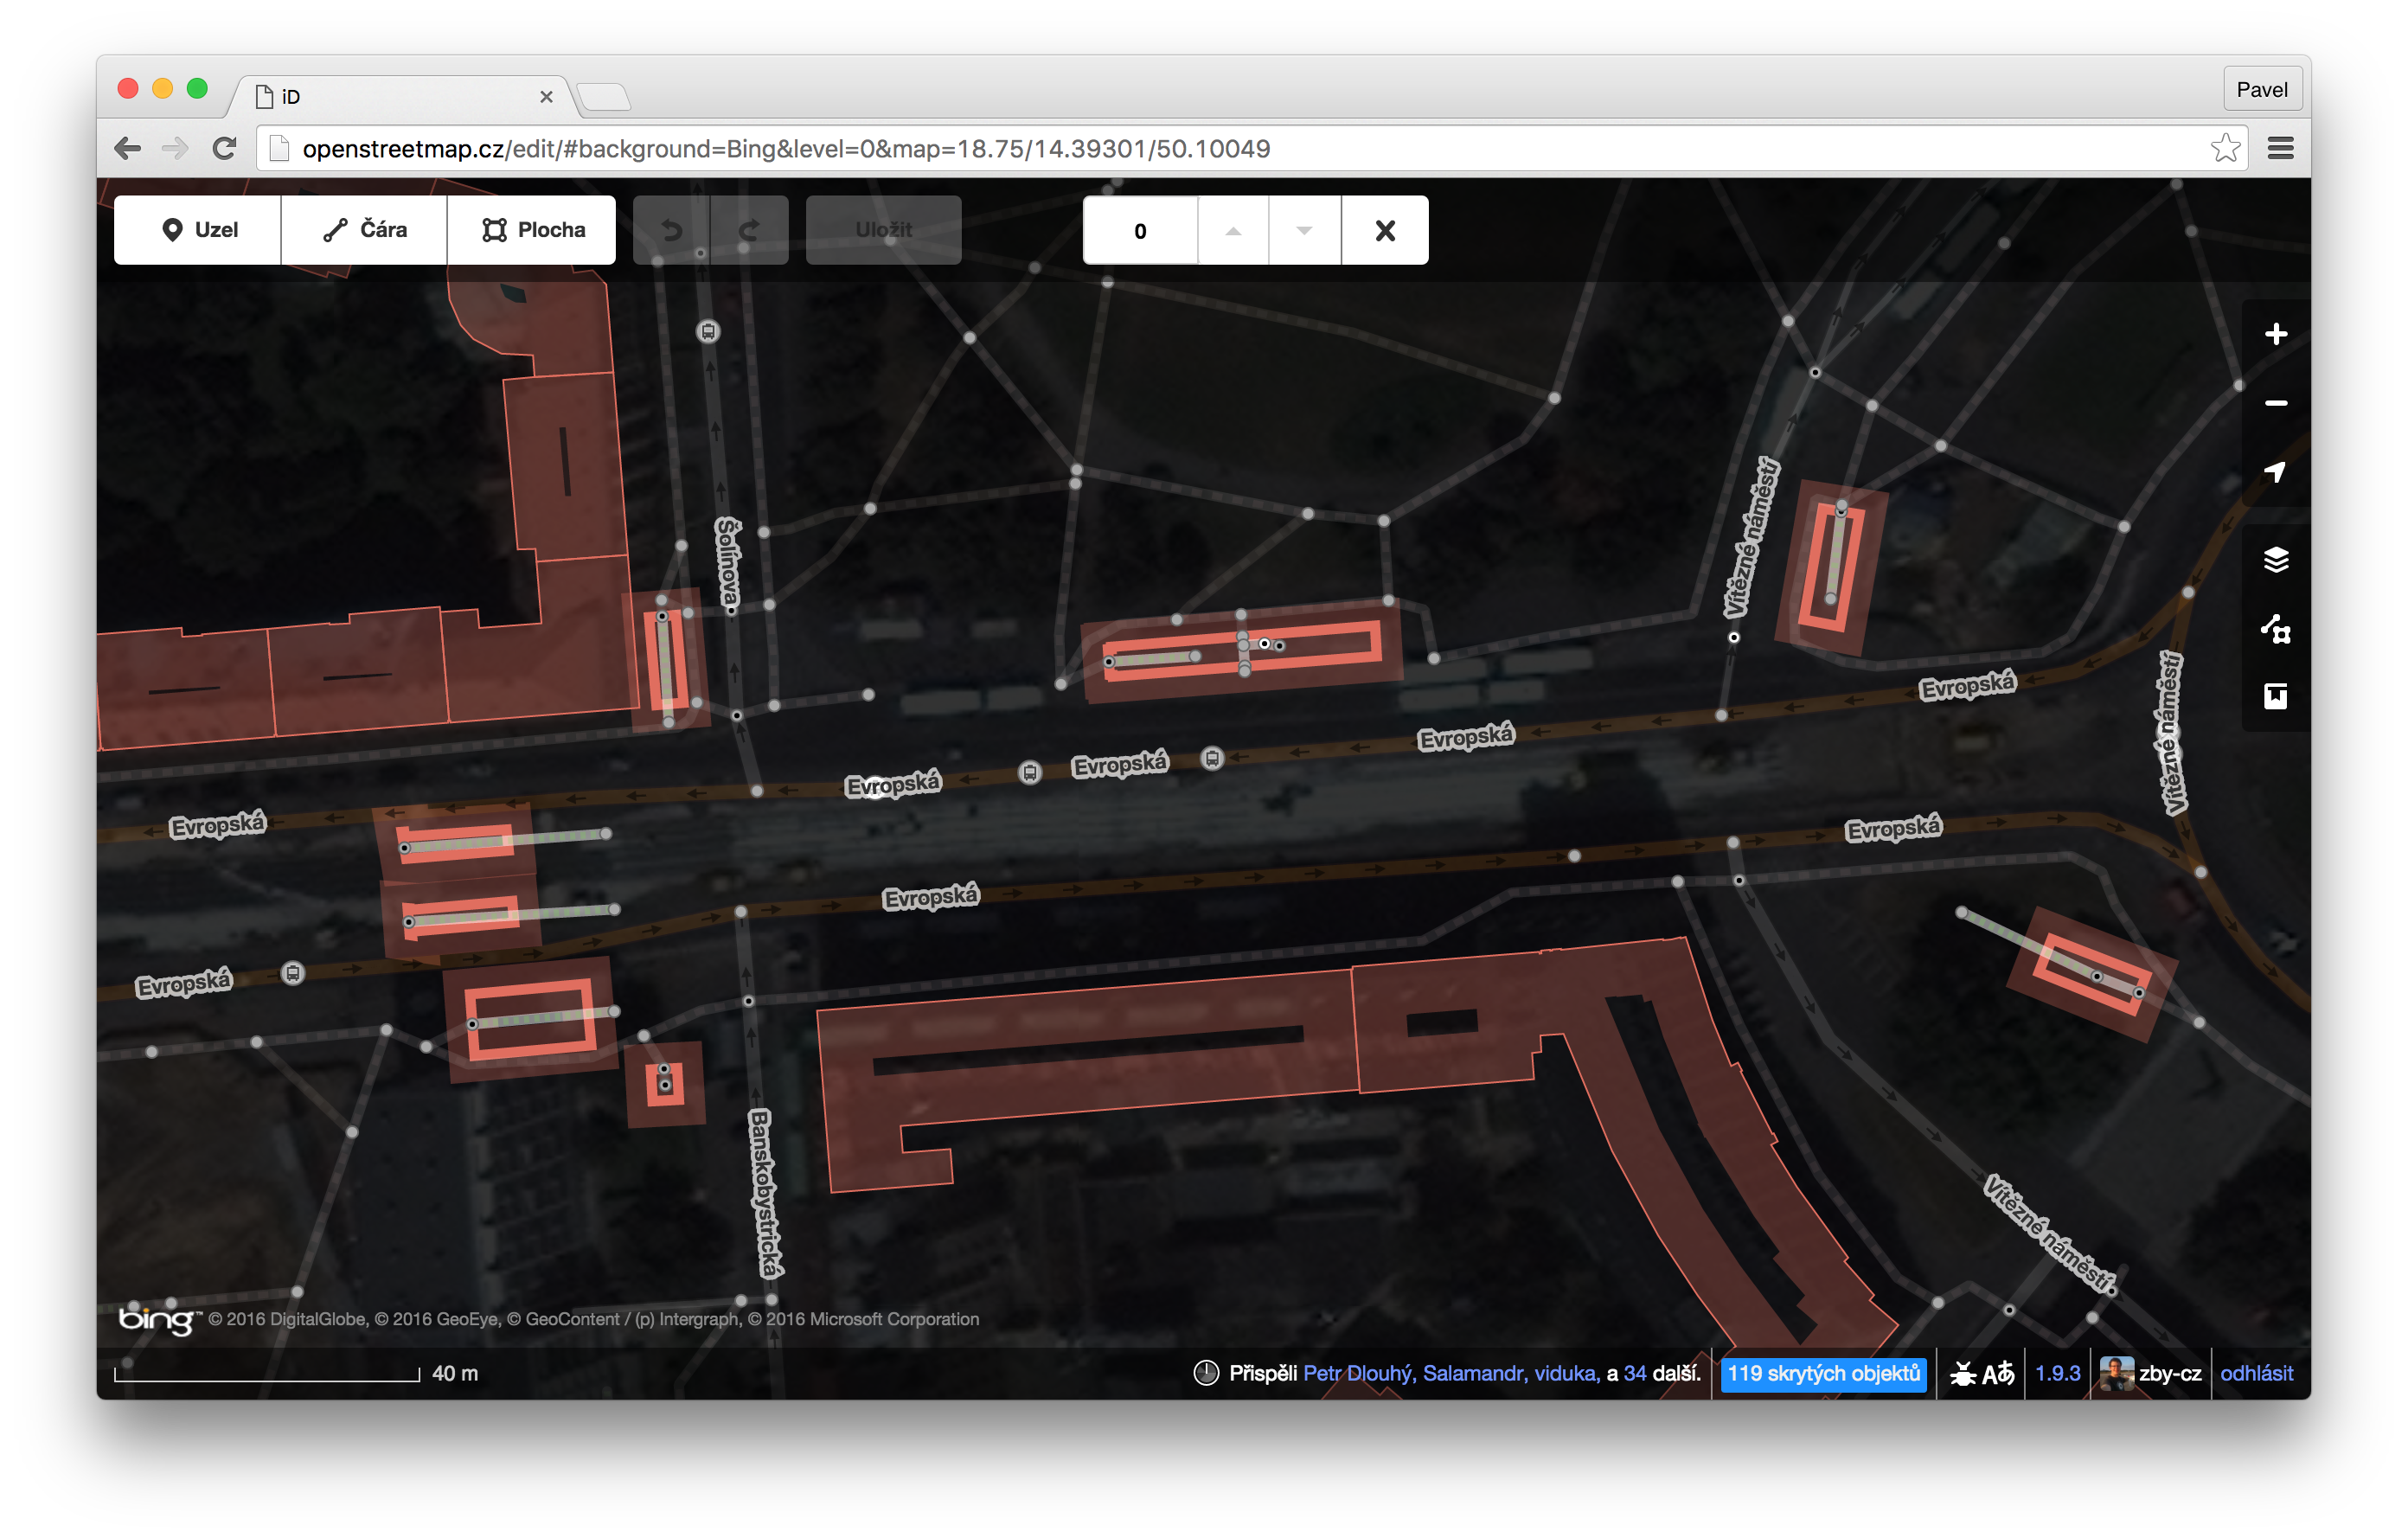
\includegraphics[width=.7\linewidth]{img/41a.png}}\hfill
                    \subfloat[\label{obr41b}]
                    {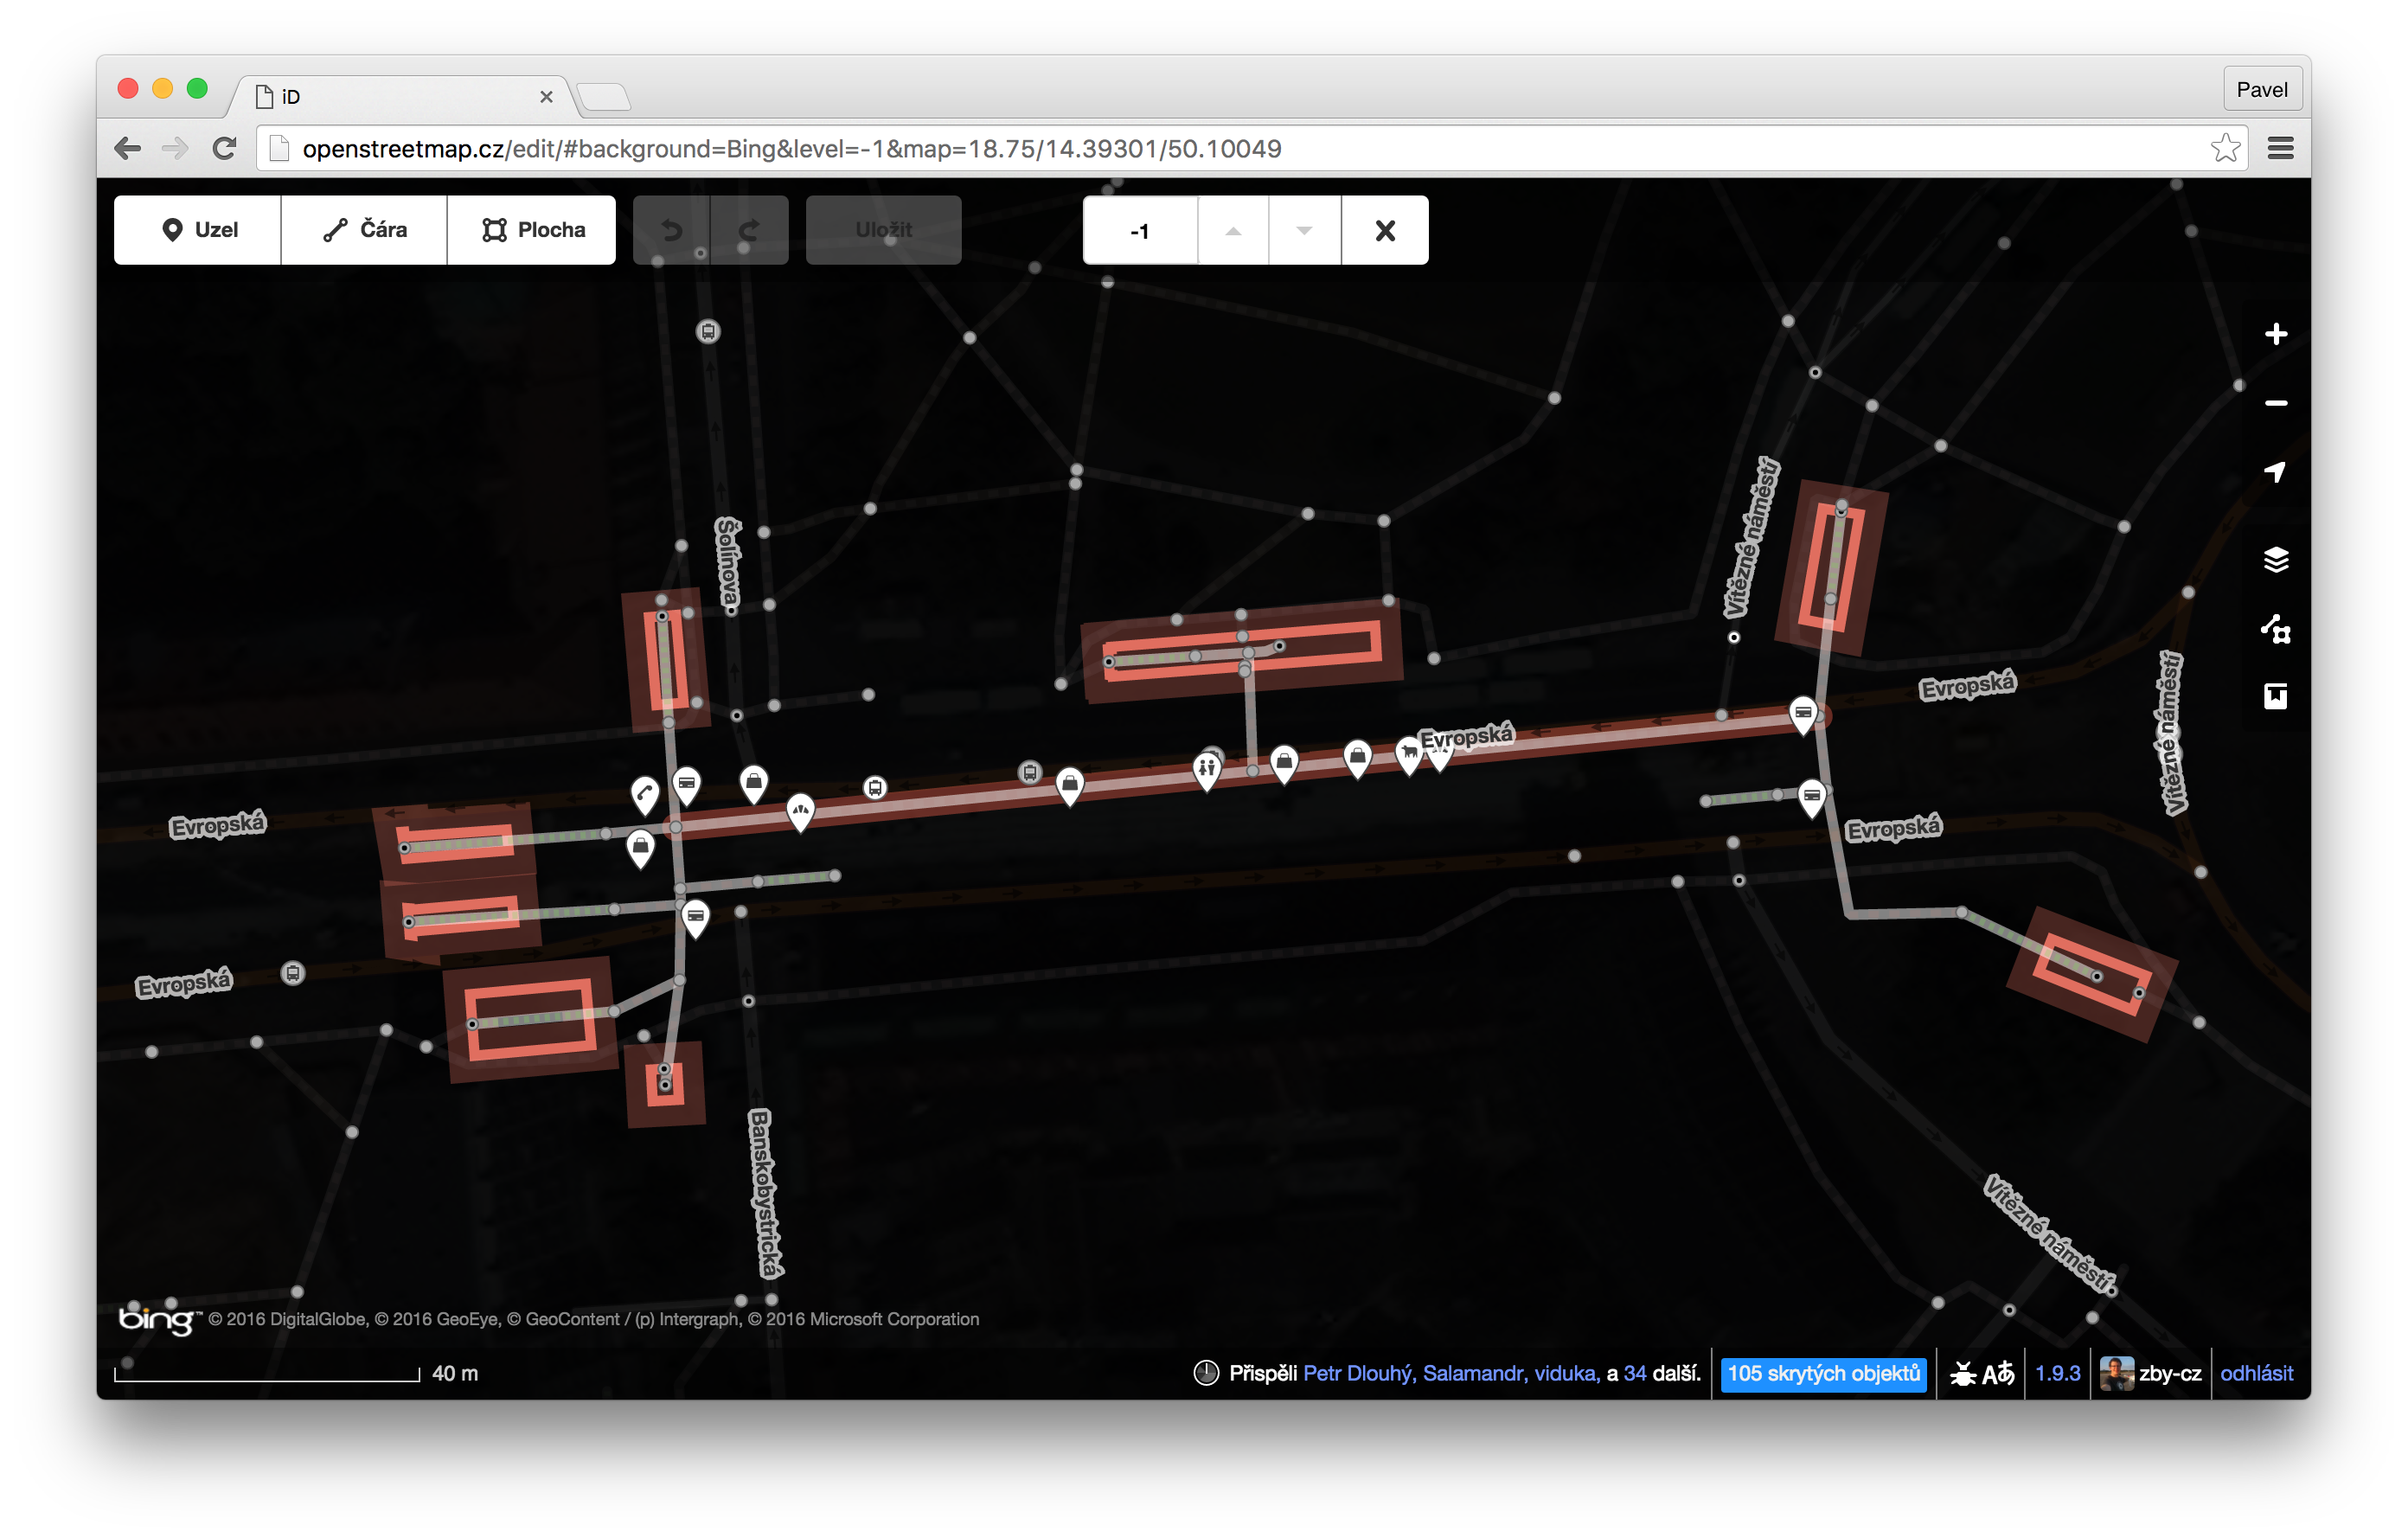
\includegraphics[width=.7\linewidth]{img/41b.png}}\hfill
                    \subfloat[\label{obr41c}]
                    {\includegraphics[width=.7\linewidth]{img/41c.png}}

                    \caption{Ukázka zmapované stanice metra Dejvická v~patře 0 (a); patře -1 (b); a bez aktivovaného indoor módu (c)}
                    \label{obr41}
                    \end{figure}
                    


                      \begin{figure}
                    
                    \subfloat[\label{obr43a}]
                    {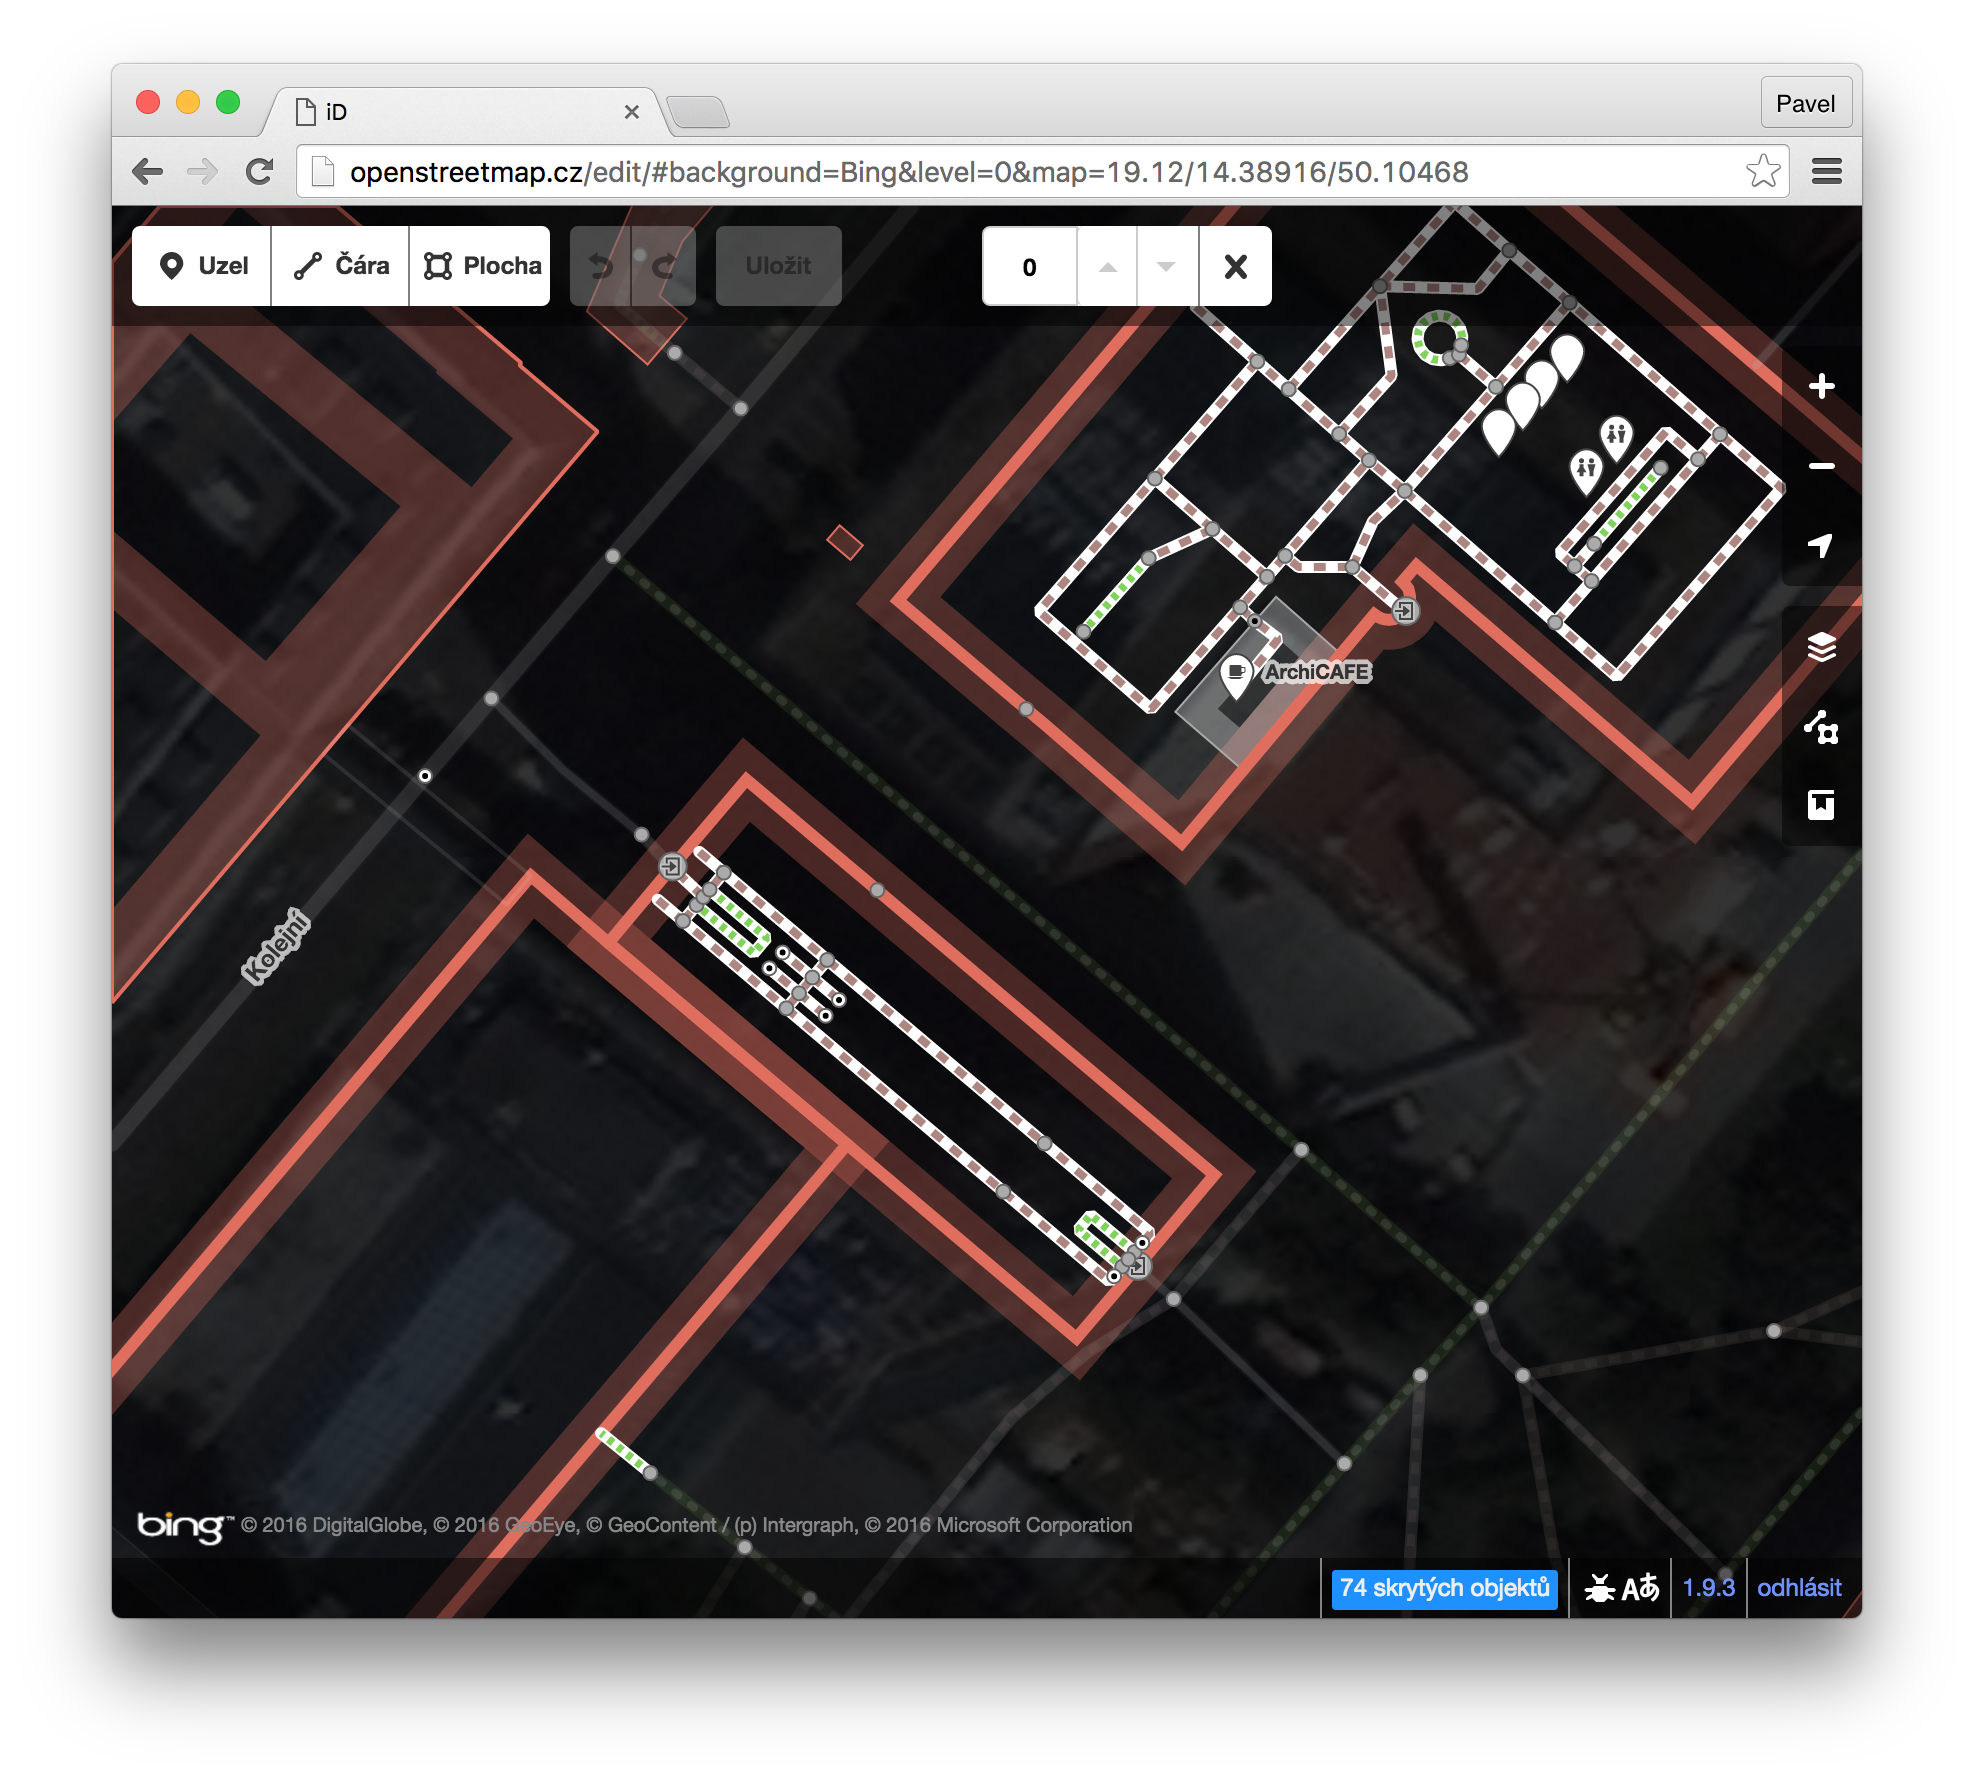
\includegraphics[width=.5\linewidth]{img/43a.png}}\hfill
                    \subfloat[\label{obr43b}]
                    {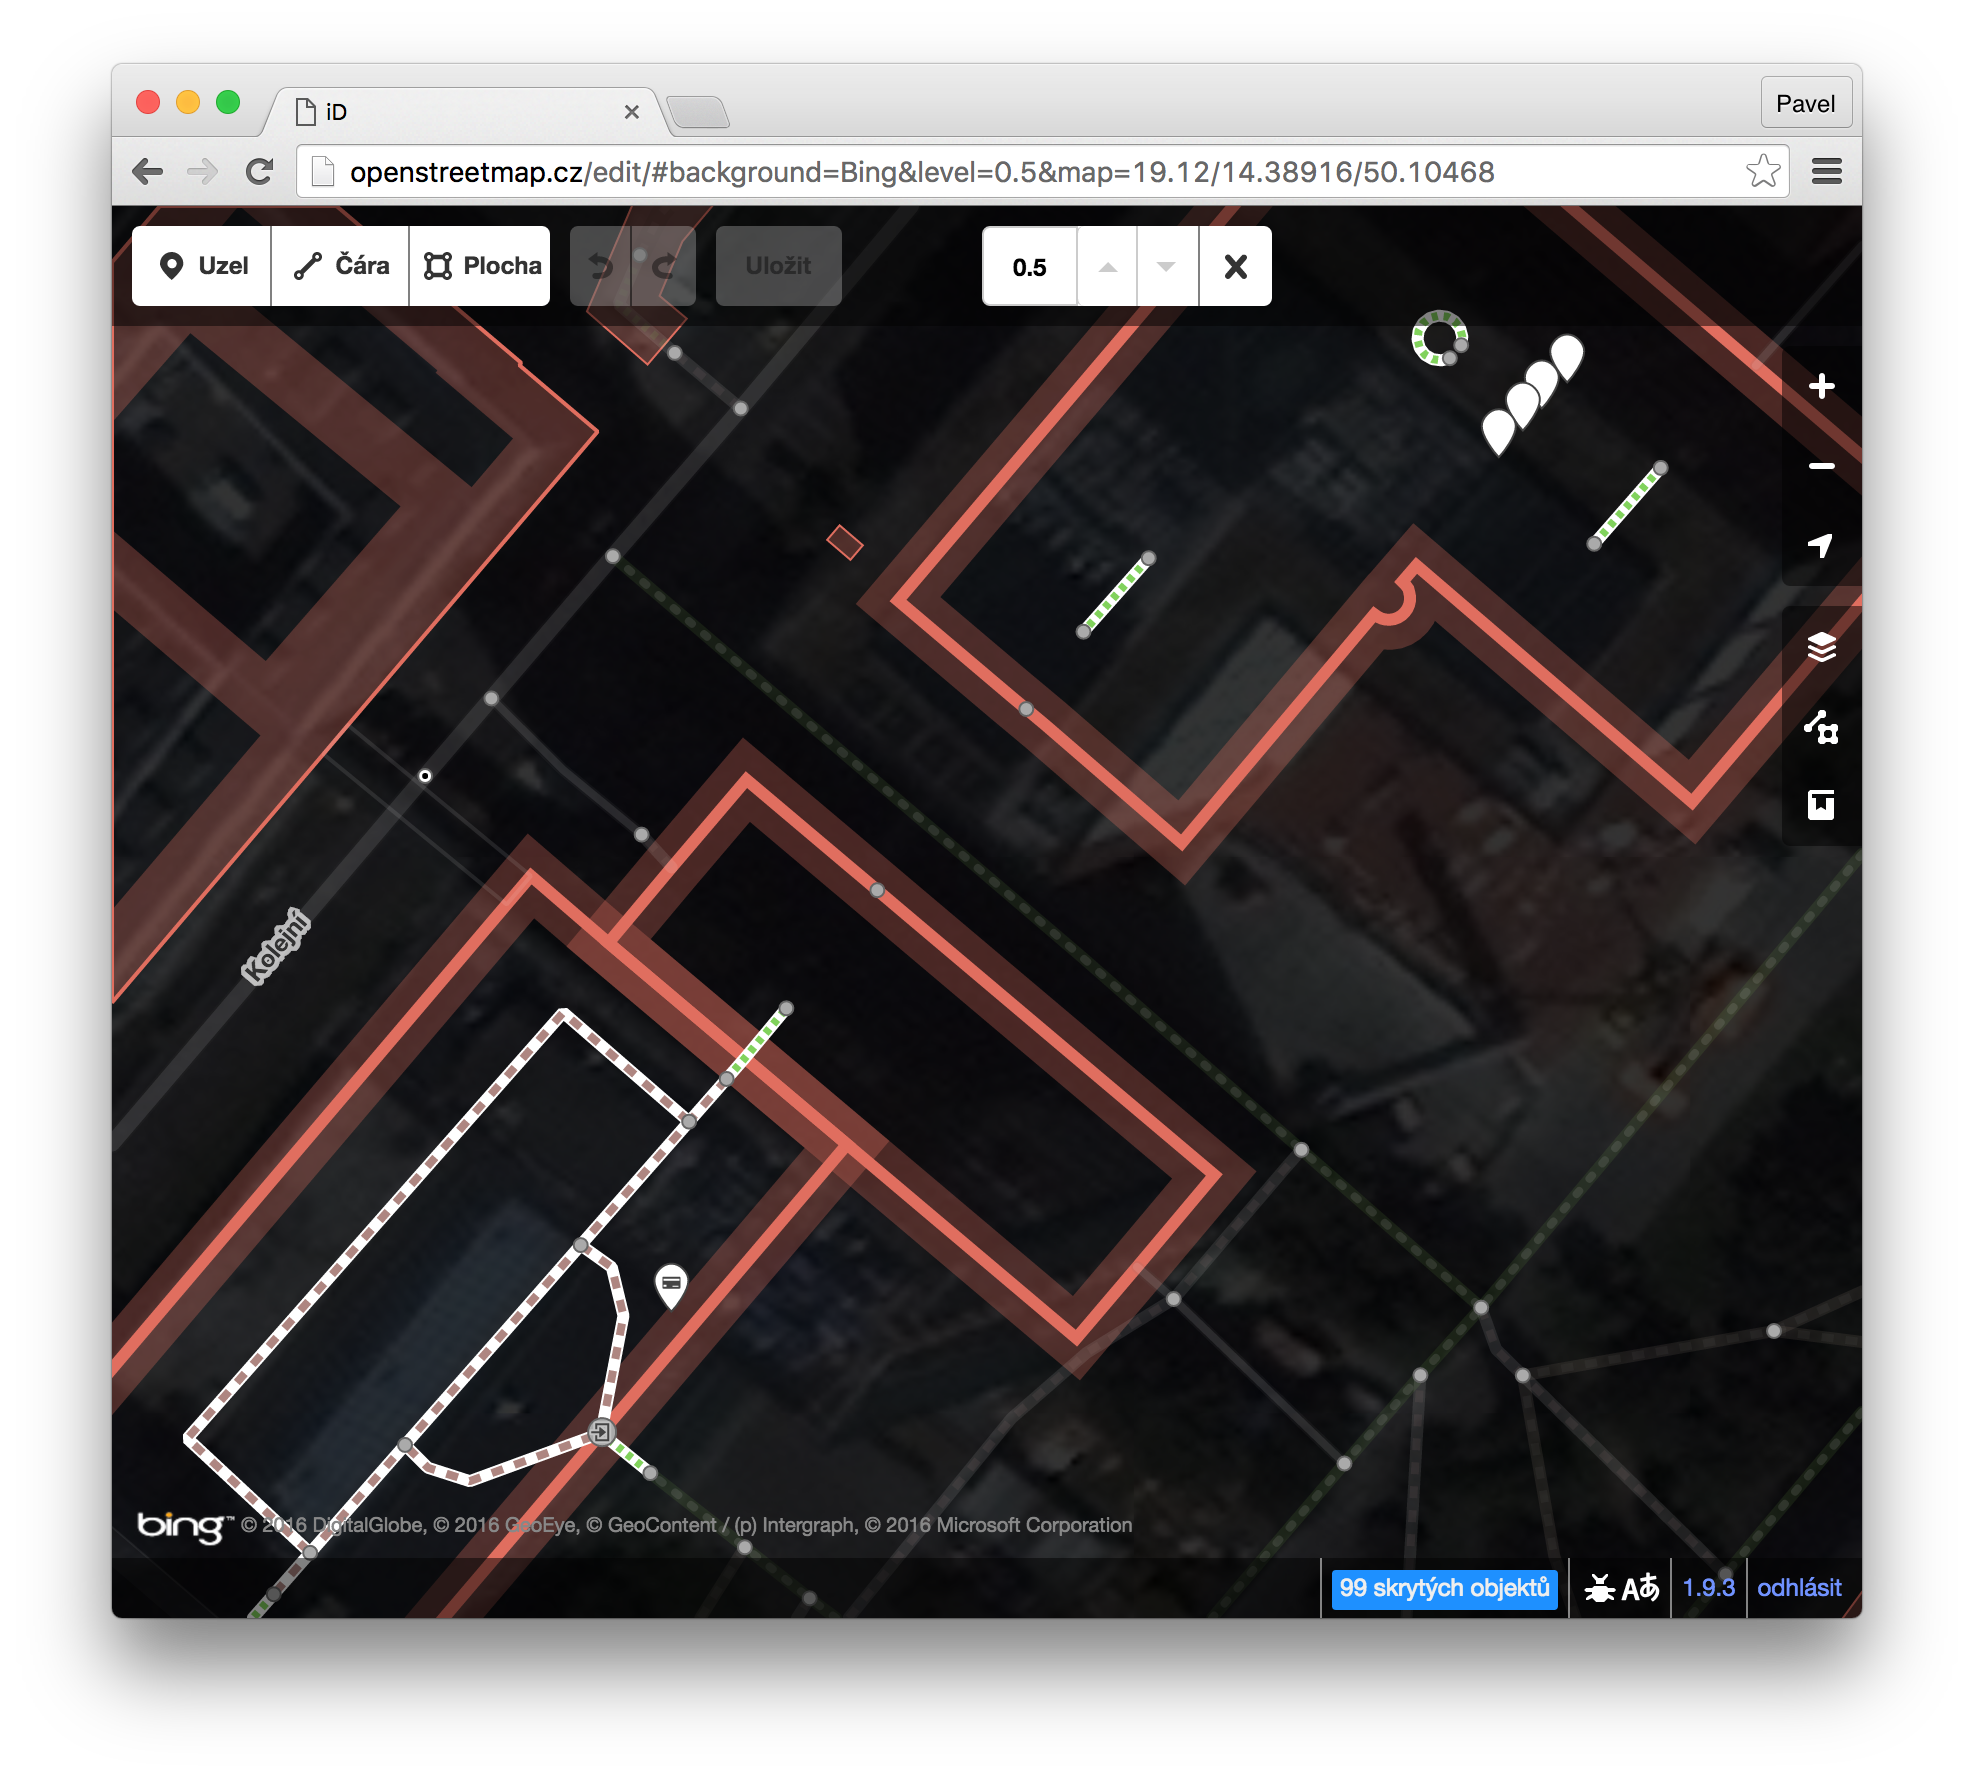
\includegraphics[width=.5\linewidth]{img/43b.png}}\hfill
                    \subfloat[\label{obr43c}]
                    {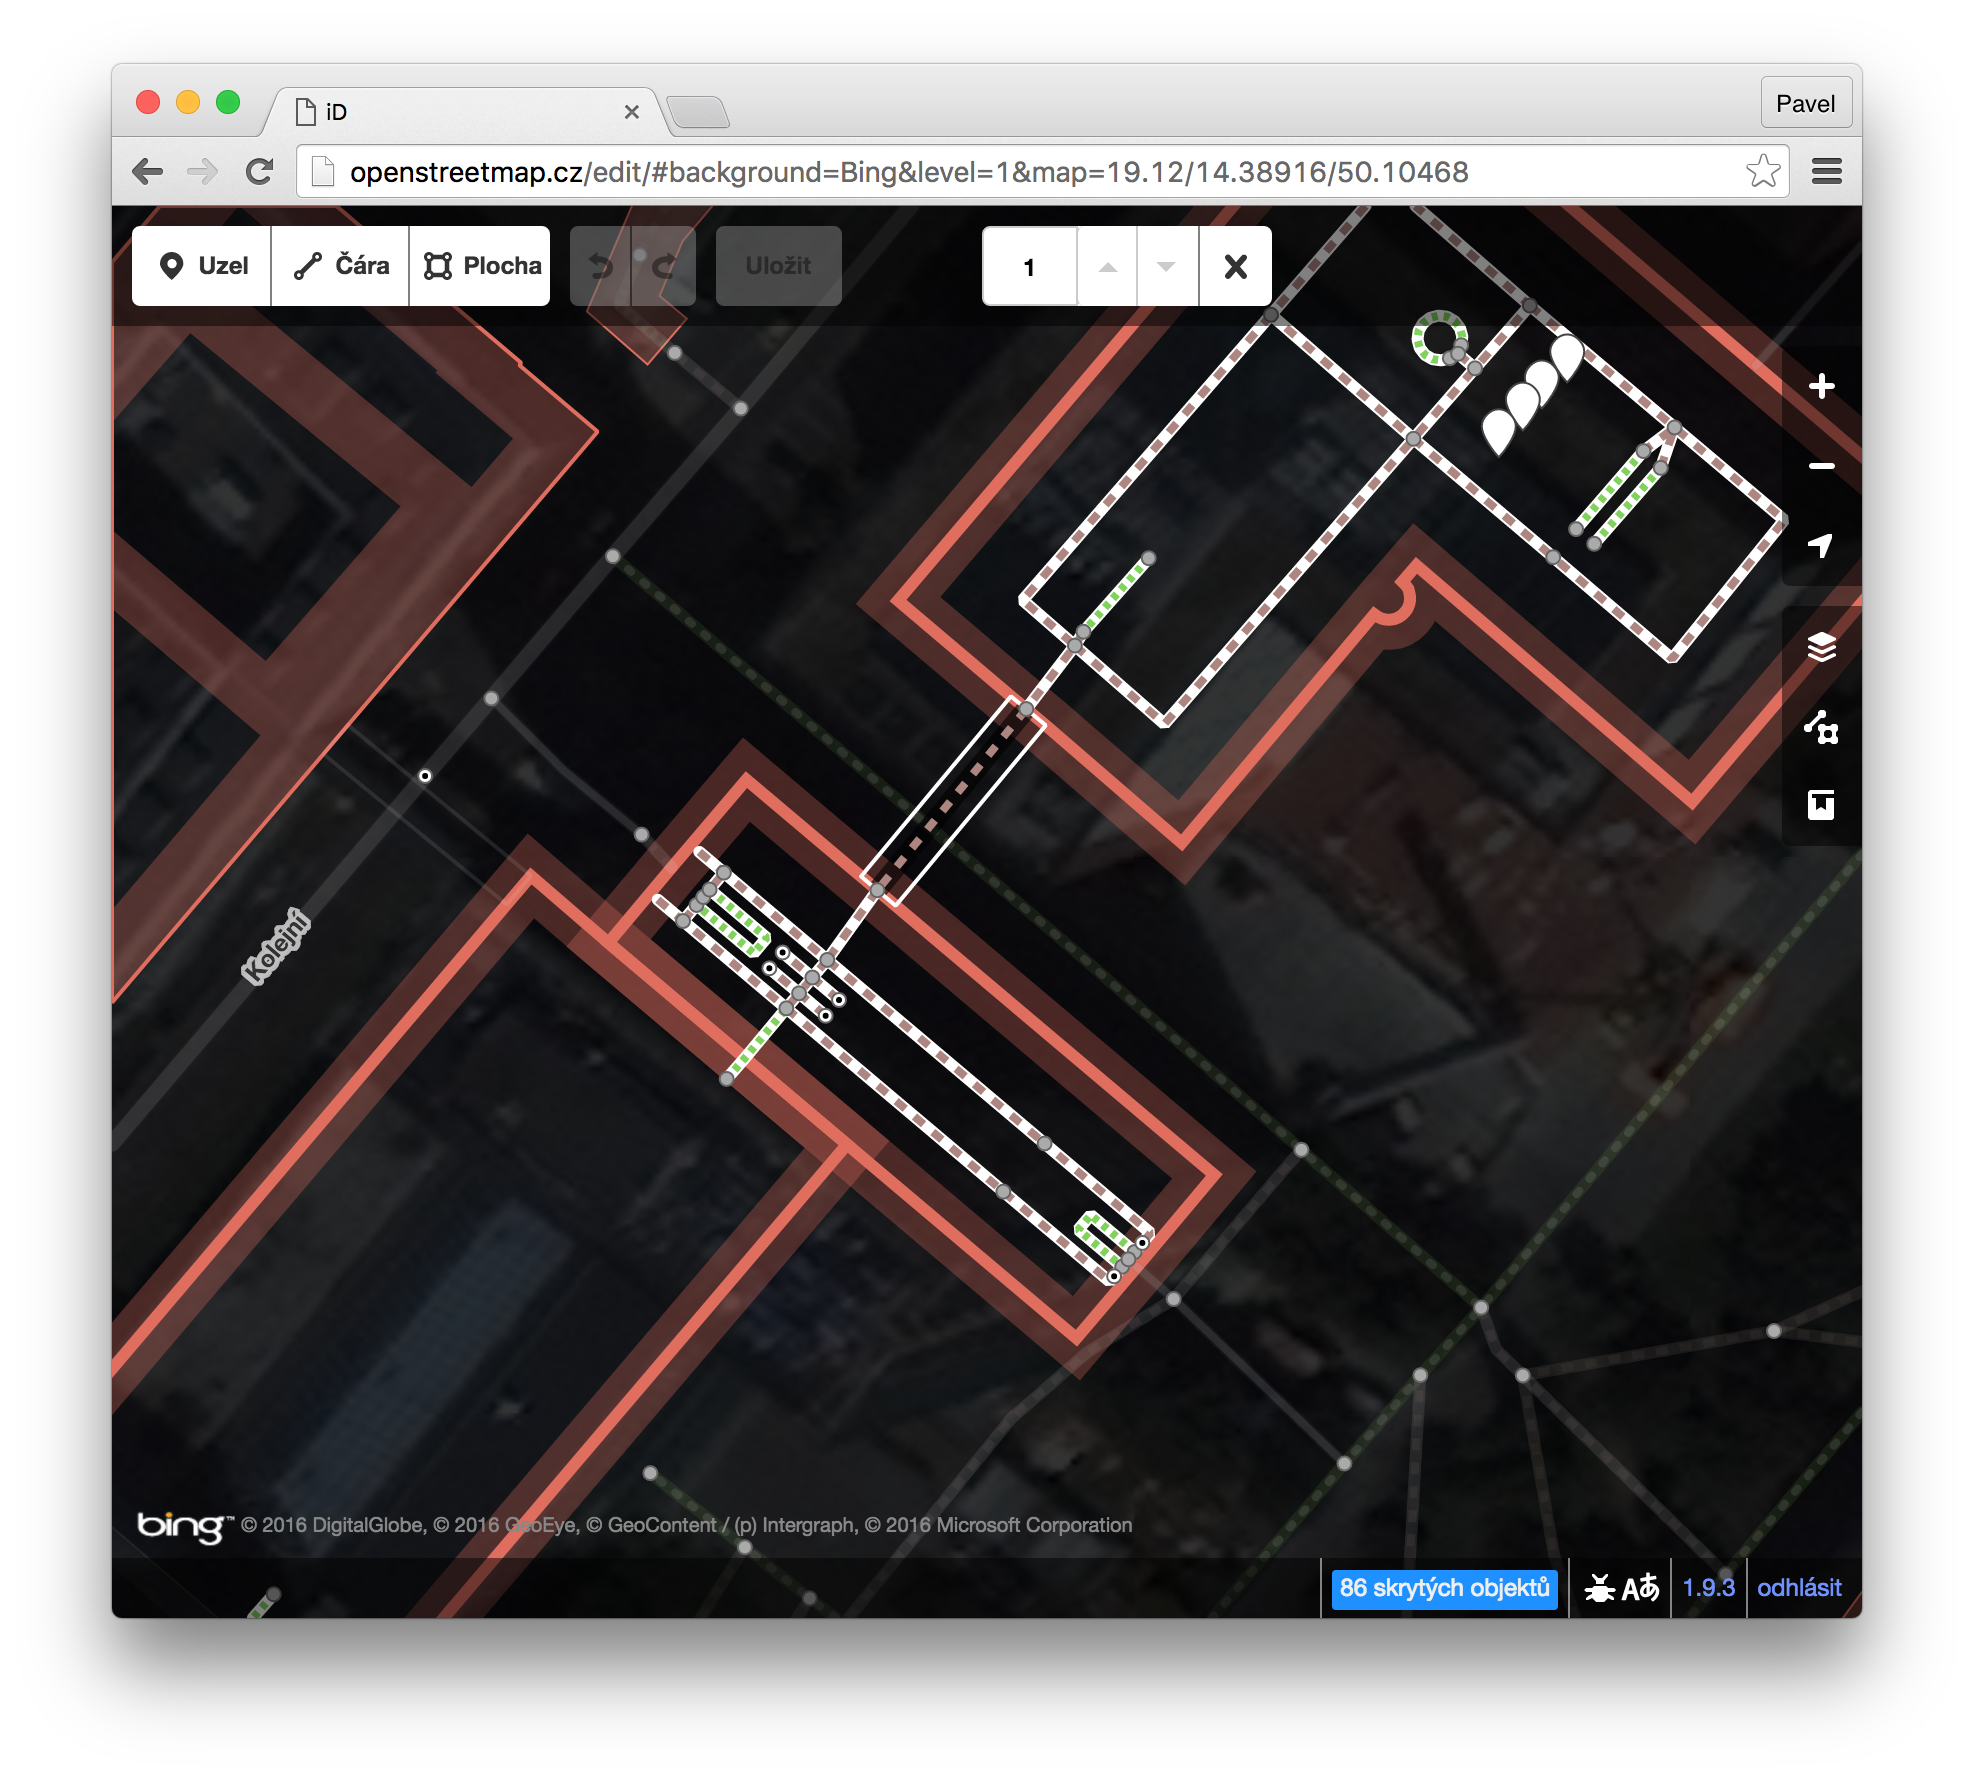
\includegraphics[width=.5\linewidth]{img/43c.png}}\hfill
                    \subfloat[\label{obr43d}]
                    {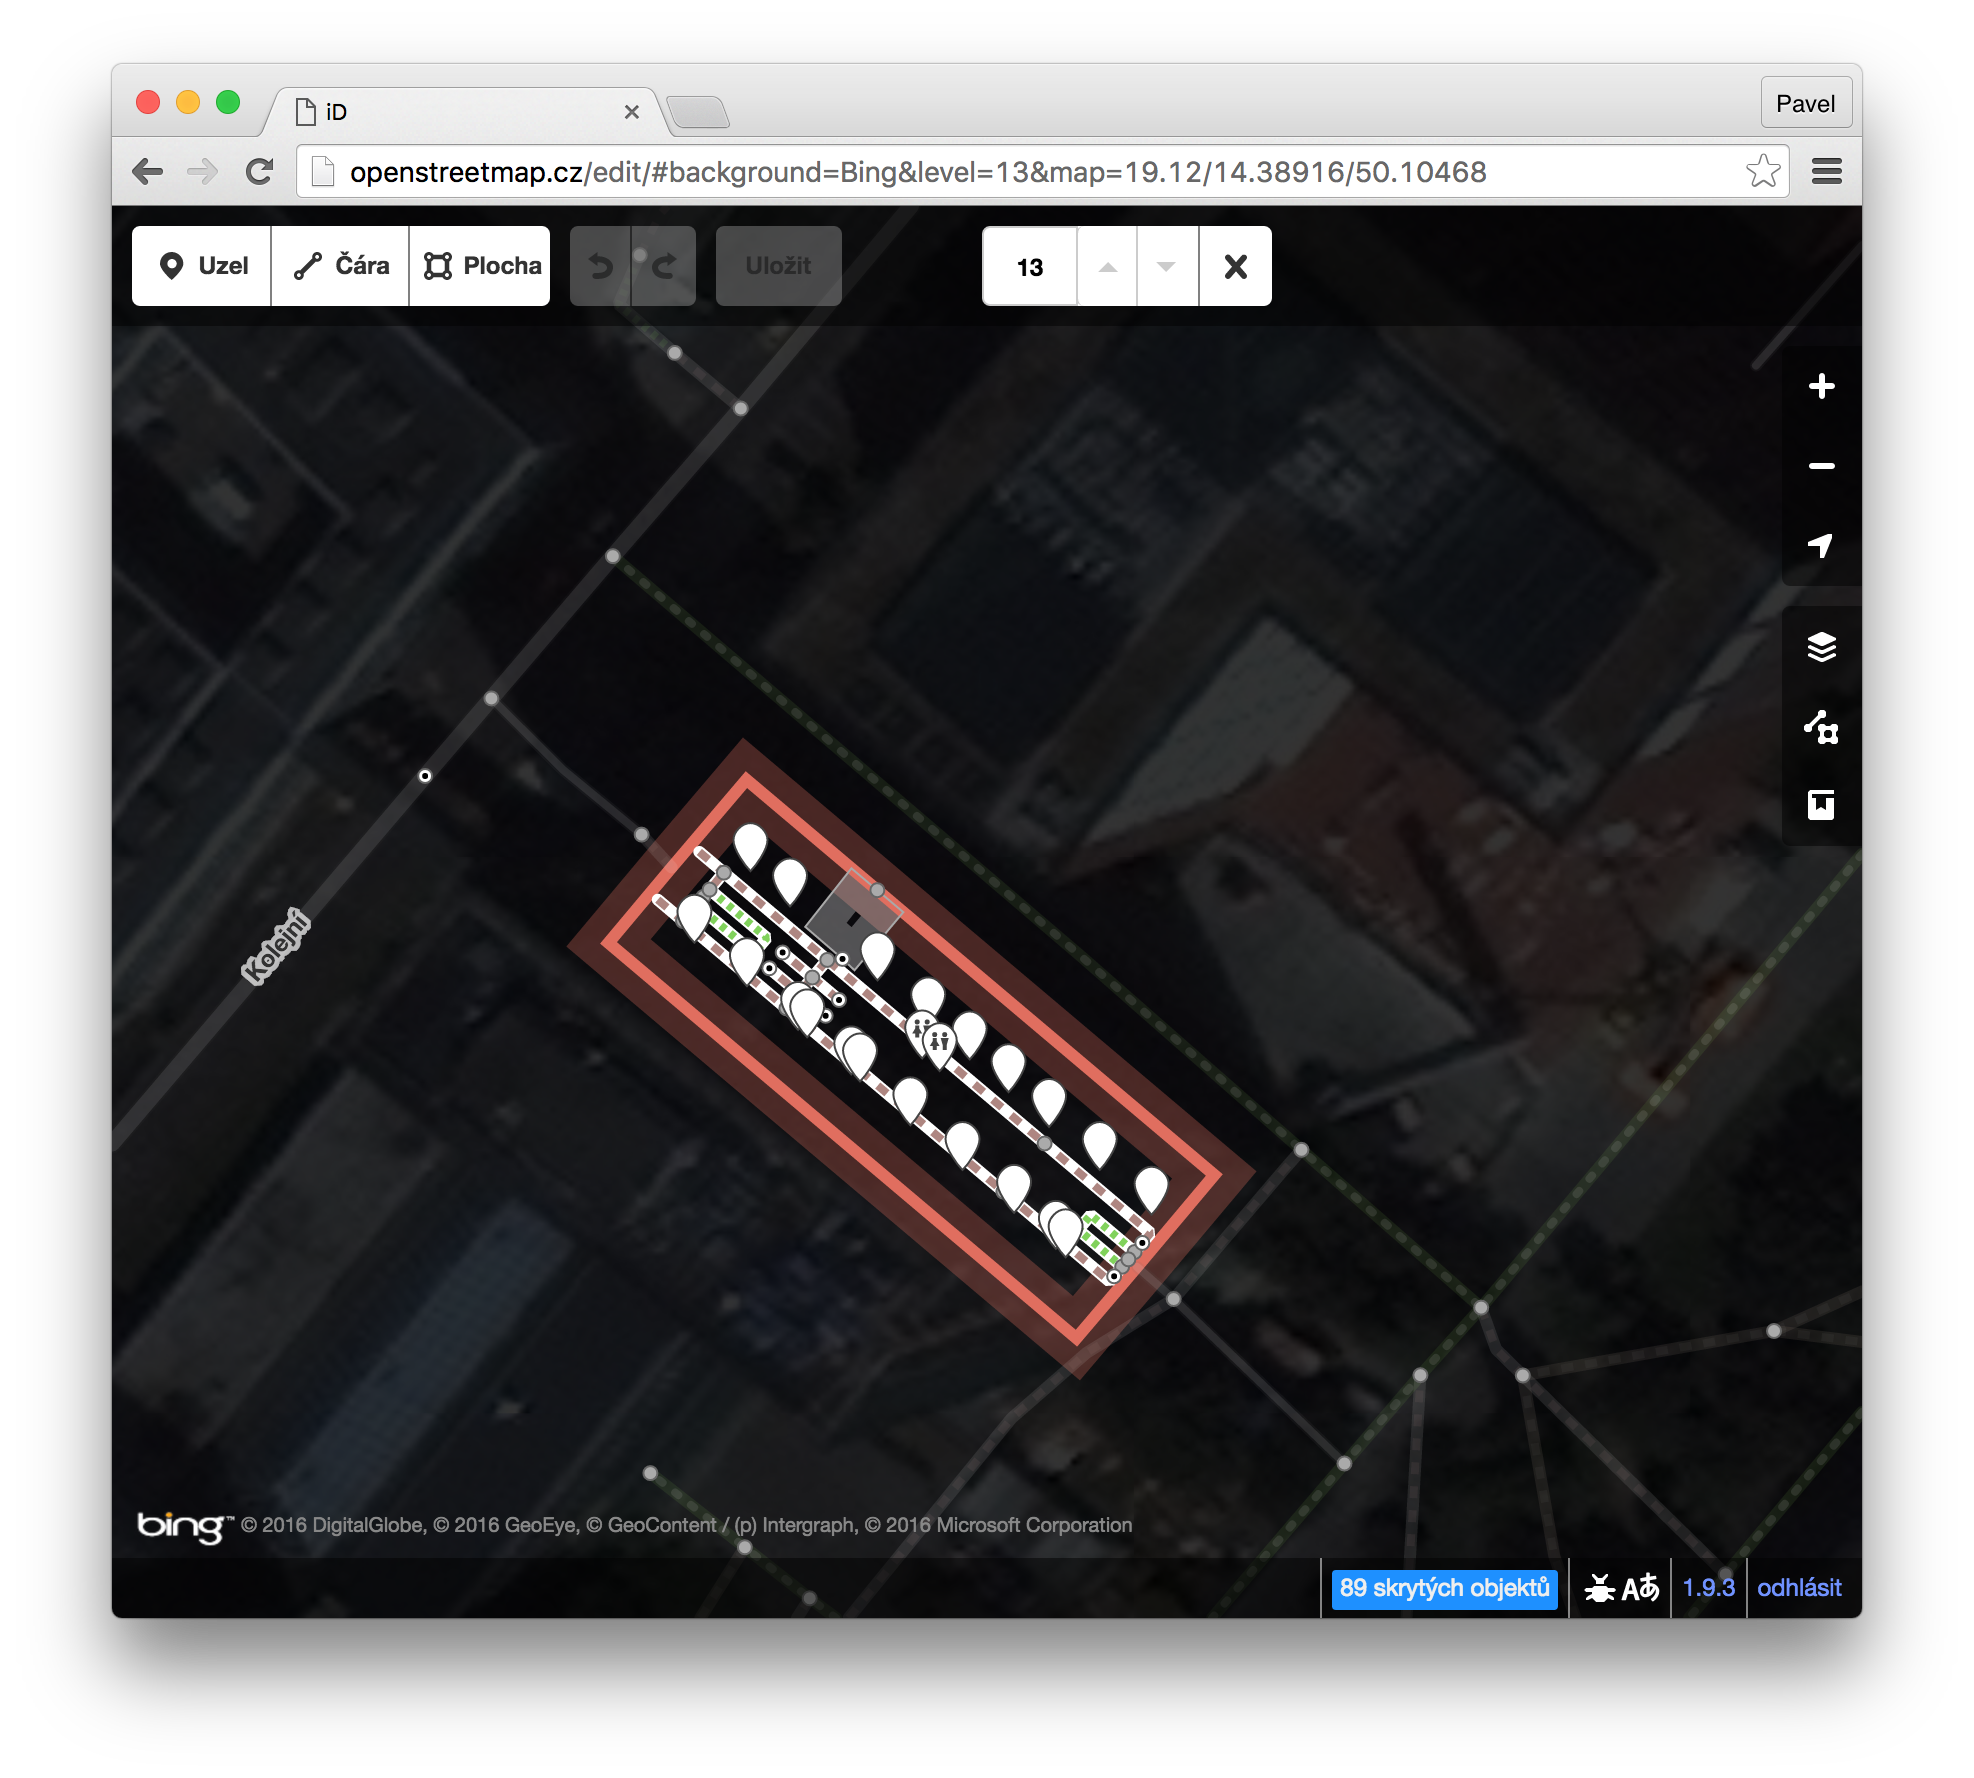
\includegraphics[width=.5\linewidth]{img/43d.png}}

                    \caption{Ukázka základního zmapování dvou budov ČVUT v~patře 0 (a); v~patře 0.5 (b); v~patře 1 (c); a v~patře 13 včetně vstupů do místností (c)}
                    \label{obr43}
                    \end{figure}
                    

\section{Řešení pro veřejné instituce}\label{ux159eux161enuxed-pro-veux159ejnuxe9-instituce}

Tato~práce může významě pomoci orientaci návštěvníků ve veřejných budovách, např. školách, úřadech~či~muzeí. Díky crowd-sourcingové povaze OSM je jen otázkou času, než data přispěvatelé vytvoří. Výsledky pak budou k~dispozici ve všech projektech, které naši metodiku implementují. Kromě celosvětového webového prohlížeče indoor map může být rozšířena i jedna z~mobilních aplikací\footnote{např. multiplatformní aplikace maps.me či Osmand}, které zatím zobrazují jen venkovní mapy.

Pokud by veřejná instituce chtěla být autoritativním zdrojem dat, je možná i varianta nasazení vlastní instance OSM databáze pouze pro tato data. Díky tomu pak může regulovat přístup uživatelů i editace. V~takovém případě bychom velmi doporučovali nastavit jednosměrný export dat do OSM, aby data byla přítomna i v~globální databázi.

\section{Webový prohlížeč indoor map}\label{webovuxfd-prohluxedux17eeux10d-indoor-map}

Jakmile jsou dostupná data, nabízí se možnost začít vytvářet vizualizace. V~tomto směru navrhujeme pouze koncept webového prohlížeče -- viz obrázek \ref{obr42}.

 \begin{figure}
	  \centering
      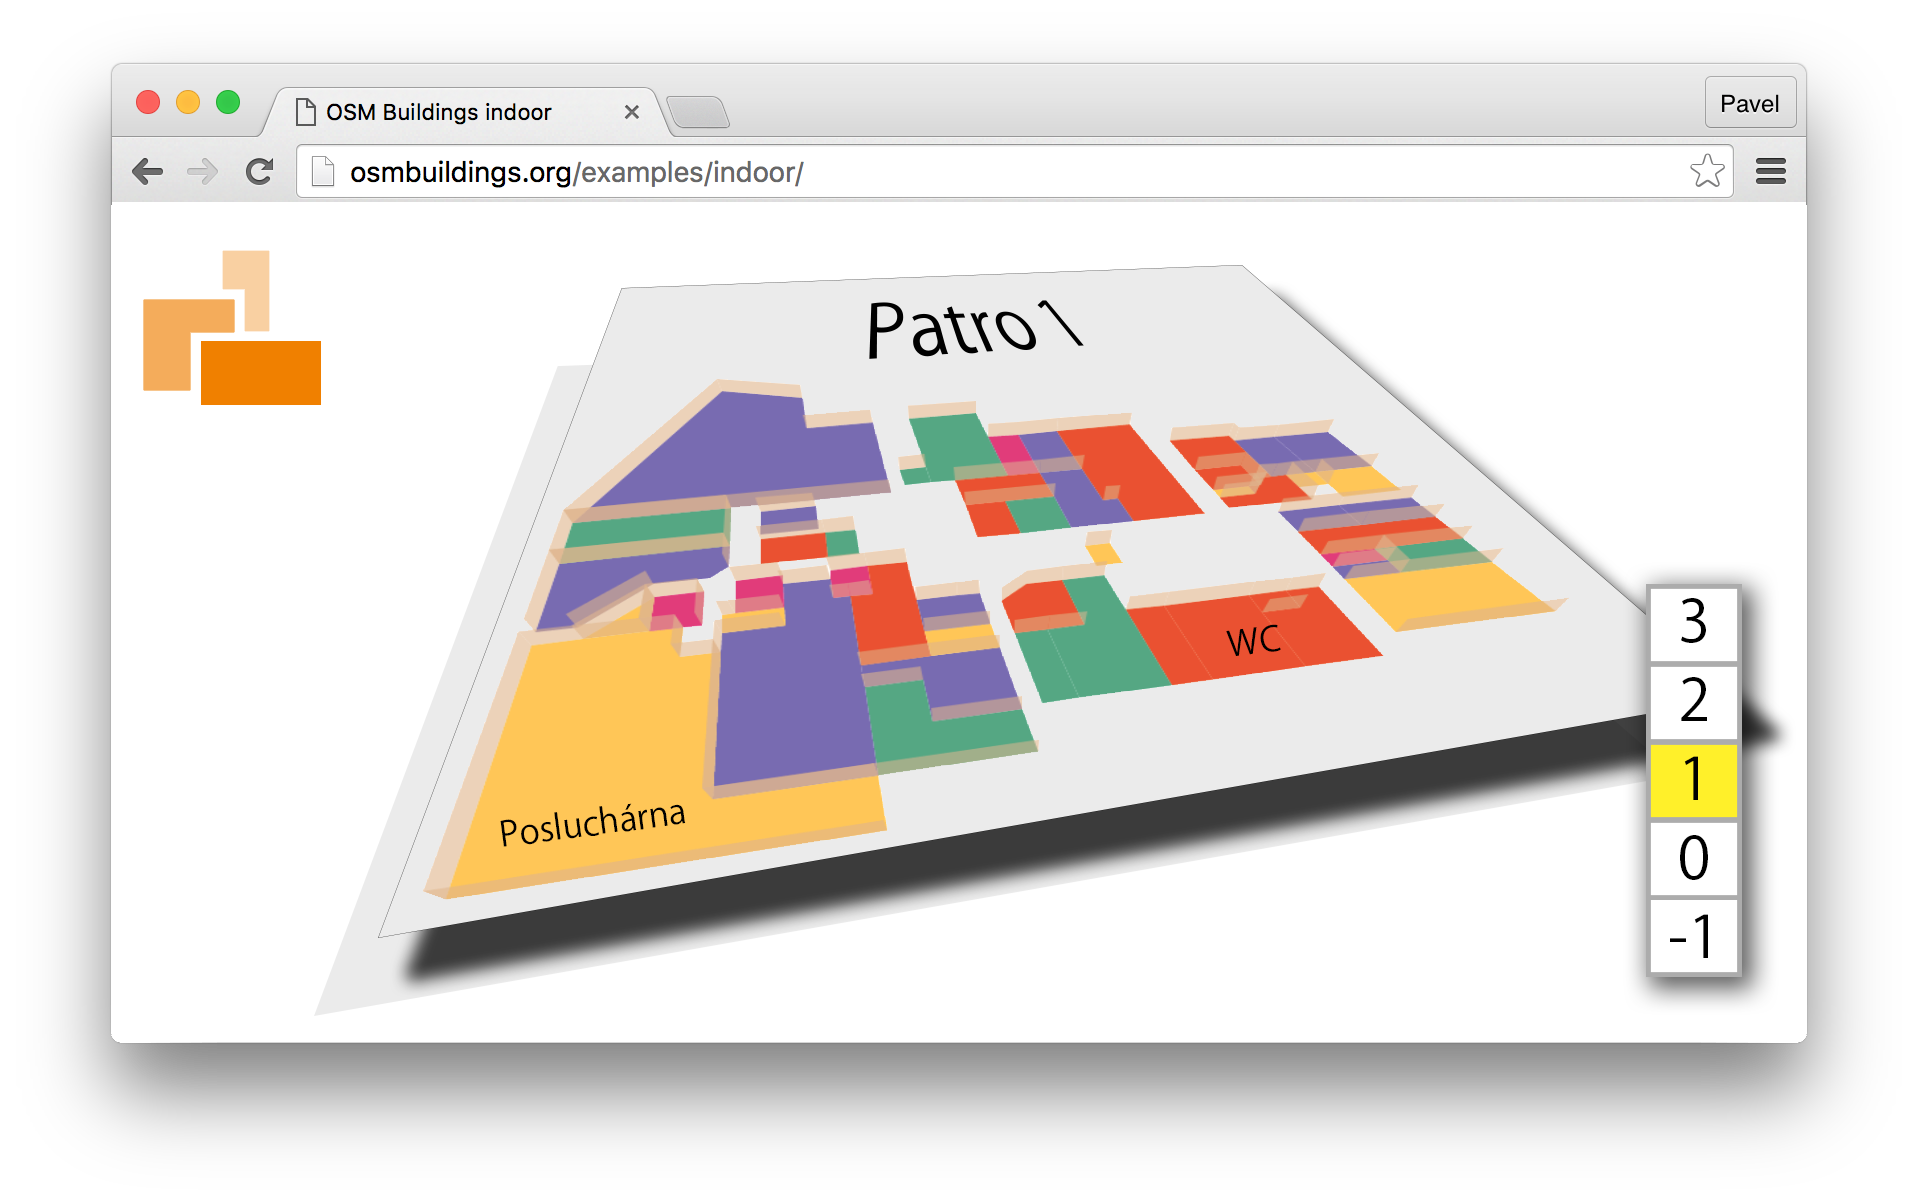
\includegraphics[width=\textwidth]{img/42-osmbuilding-indoor-upraveny.png}
      \caption{Koncept 3D prohlížeče -- upraveno v~grafickém editoru}
      \label{obr42}
  \end{figure}

\begin{conclusion}

Problematika indoor map se ukázala jako velké téma dnešní doby. Platforma OpenStreetMap v~posledních letech zaznamenala velký rozmach, ale vhodný návrh pro indoor mapování dosud nebyl přijat. Řešení, které je výsledkem této práce, má~potenciál OSM vhodně rozšířit, a umožnit~tak~tvorbu celosvětové indoor mapy spravované uživateli.

V~práci se rozsáhle věnujeme problematice indoor map a geolokaci, shrnujeme vývoj v~komerční i open-sourcové sféře a ukazujeme i několik zajímavých projektů pro další využití.

Popsali jsme architekturu OpenStreetMap, se kterou máme dlouholeté zkušenosti, prošli a zhodnotili všechny dosud zveřejněné návrhy pro indoor~a nakonec navrhli vlastní metodiku. Vyšli jsme z~aktuálního systému Simple Indoor Tagging a navrhli některá zjednodušení pro snazší zadávání uživateli. Systém byl odzkoušen nejprve ve stávajícím editoru JOSM a poté bylo namodelováno několik případů v~námi upraveném editoru iD. Metodiku se chystáme navrhnout jako oficiální tagování pro OSM.

Editor iD se ukázal jako vhodný kandidát na doplnění funkcionality. Popsali jsme jeho architekturu, navrhli a otestovali uživatelské rozhraní a pokusili se o~začlenění do distribuce. Správce projektu naši úpravu shledal s~pozitivním ohlasem a chce spolupracovat na začlenění.

Nabídli jsme řešení vhodné pro veřejné instituce a máme v~plánu další rozvoj. Aktuálně připravujeme spolupráci~s~ČVUT Navigátorem, a také s~Národním muzeem, které v~minulosti projevilo zájem o~indoor navigaci a lokalizaci pomocí QR kódů.

\end{conclusion}